%!TEX root = ../../../../thesis.tex

\section{Preliminary Simulation Results}

	In this section we present the results of preliminary \emph{in silico} explorations of the discretized model presented in \Fref{sec:discrete}. We investigate several different basic circuits of \Pes and discuss our findings. The circuits are based on small graphs in the hope that one may still reason about them analytically. This is a preparatory step to towards a better understanding of the behavior of our model. Ultimately, the hope is to gain insights useful for deriving an algorithm based on the model.

	The following facts suggest, that our implementation is correct: First, we find that during the execution of our model Kirchoff's laws are obeyed. Second, the implementation maintains the distinct invariants we have established analytically as given by \Fref{lem:inv_cont}. Finally, for converged cycles of \Pes we observed precisely the behavior predicted by \Fref{lem:ring_cont}. This constitutes a nice example of how numerical simulation and analytical work are in an symbiotic relationship. Insights gained in one frequently suggest directions of exploration to the other. 

	All the topologies we present are drawn as directed graphs. The orientation of an edge $e = (x,y)$ corresponds to the definition of the \Pe given in \Fref{fig:vein}. We stress that the orientation has no effect on the results of the simulation since \Pes are symmetric as are the chosen initial conditions. In the plots presented shortly we always show the value of $i_p$ for all involved \Pes to illustrate the current flow. Thus if $i_p > 0$ current flows in the direction the edges is oriented to, \ie from node $x$ to node $y$. The reverse is true if $i_p <0$. This information is important when interpreting how the flows split up at junctions of the \Pn.

	Unless noted otherwise, all presented simulations were initialized with the same starting values for all \Pes. The only exception are the initial capacitor voltages which were set at random. They are summarized in \Fref{tab:initialization}\footnote{Unfortunately, many plots appear to start at $i_p(r=0) \neq 0$ instead of $i_p(r=0) = 0$. This illusion is the product of the circuits instantly jumping from $i_p(r=0) = 0$ to $i_p(r=1) \neq 0$ in a single round.}. The number of executed rounds can be read off the plots directly. 

	\begin{table}
        \centering
        \begin{tabular}{@{} l *2l @{}}
        \toprule
         \multicolumn{1}{c}{Property}    & value  \\ 
        \midrule
         $u_p = u_p'$ & $0$   \\ 
         $i_p = i_p'$ & $0$   \\ 
         $u_C$ & rand. uniform real $u_C \in [ -0.5 , 0.5 )$   \\ 
         $C$ & $10$ \\
         $R$ & $1$ \\
         $\hat{U}$ & $1$ \\
         $\alpha$ & $(R C)^{-1}$ \\
         $\beta$ & $3 R$ \\
         $x = y$ & 1 \\
        \bottomrule
        \end{tabular}
        \caption[Simulation - Initial values]{Initial settings for discrete simulations at $r=0$.}
        \label{tab:initialization}
     \end{table}

     For some topologies we observe periodic oscillations. To determine the period of these oscillations we explored three different methods of period detection. They are based on signal auto-correlations, FFT and simply determining the distance between subsequent peaks respectively. It turned out that while all three methods usually agree, the simplest method of extracting the period from the peaks directly yielded the most robust results and was thus adopted.

    \newpage
	\subsection{Cycle of Physarum Elements}

		We begin by investigating the behavior of a \Pn that is a cycle. Exemplary we present the result obtained for a $4$-cycle consisting of $4$ \Pes, see \Fref{fig:cycle_4}. Note that together with \Fref{fig:cycle_4_legend}, a color coding is defined which serves as a legend for the remaining plots of \Fref{fig:cycle}.

		For a converged $4$-cycle of \Pes we obtain precisely the results predicted by \Fref{lem:ring_cont}. Namely, current can either flow clockwise, counter-clockwise or not at all if the \Pn is converged. 

		These scenarios are reflected in the behavior of the capacitor voltages $u_{C,e}(t)$ given by \Fref{fig:cycle_4_uC_zero}, \Fref{fig:cycle_4_uC_positive} and \Fref{fig:cycle_4_uC_negative}. It can be seen that convergence is rapid for all three depicted cases. Note, that only in \Fref{fig:cycle_4_uC_zero} the values converge to $0$. This is the case in which the respective currents $i_{p,e}(t)$ converge to zero as well, see \Fref{fig:cycle_4_ip_zero}. The currents indicate that the flow through the entire cycle dies out. This is expected, since for this case exclusively, $\beta = R$ was chosen as a simulation parameter. As a result, currents are quickly damped to zero as can be seen in the proof of \Fref{lem:ring_cont}.

		\Fref{fig:cycle_4_ip_positive} and \Fref{fig:cycle_4_ip_negative} illustrate the remaining cases treated in said proof. For a given period the \Pes of the cycle interact to eventually ``agree'' on a common, constant value of current. This value can either be positive, leading to counter-clockwise flow through the cycle or negative, resulting in clockwise flow. At present, we do not know how the circuit decides on the sign of the current. Either the initial choice of the capacitor voltages determine the sign or it is random. This question deserves further investigation in the future.

		We have repeated this experiment for various $n$-cycles with $n \in [3,10]$ obtaining identical results. We find that edges agree rapidly on the flow for all tested $n$. It seems that for larger $n$ the circuit needs progressively longer to converge. Unfortunately, no precise statements about convergence and its dependence on the size of the cycle are available at this point.

		Finally, we remark that the above results are only valid for converged cycles. Extreme initial conditions can also be chosen such that the \Pn does not converge. For a $4$-cycle anti-phase oscillations between pairs of edges have been forced in this way.  

		\begin{figure}
			\centering
			\subfloat[][]{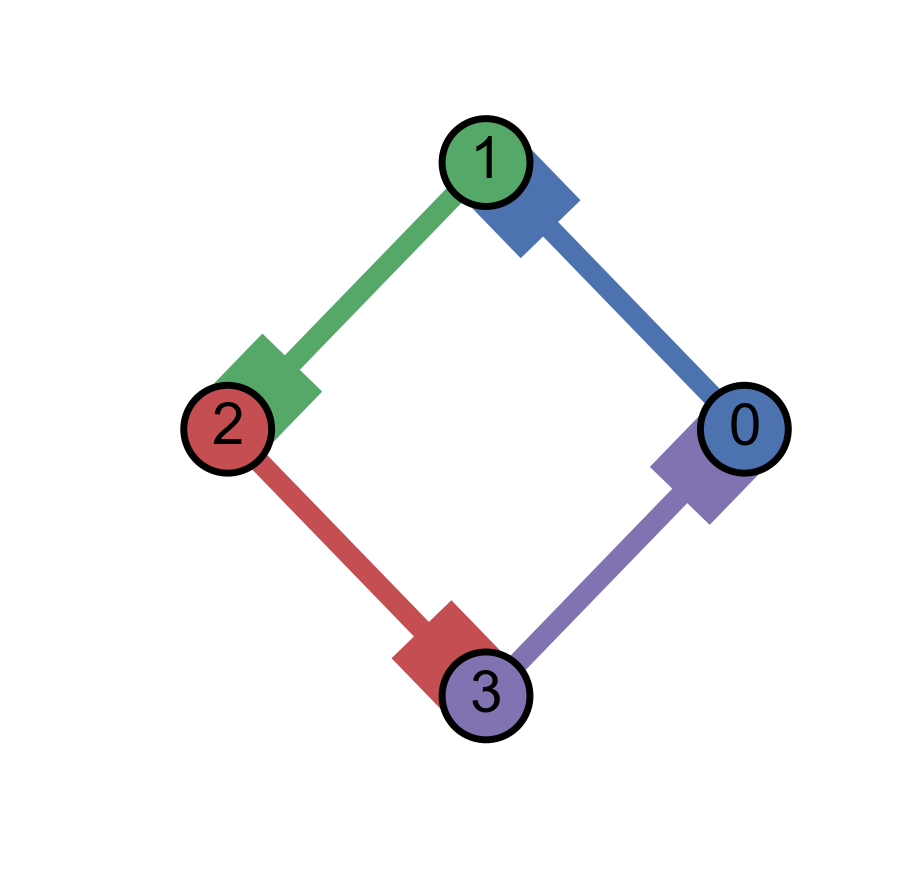
\includegraphics[width=0.4\linewidth,keepaspectratio,trim={0 3cm 0 2cm},clip]{./simulation/cycle/cycle_4.png}\label{fig:cycle_4}}\qquad
			\subfloat[][]{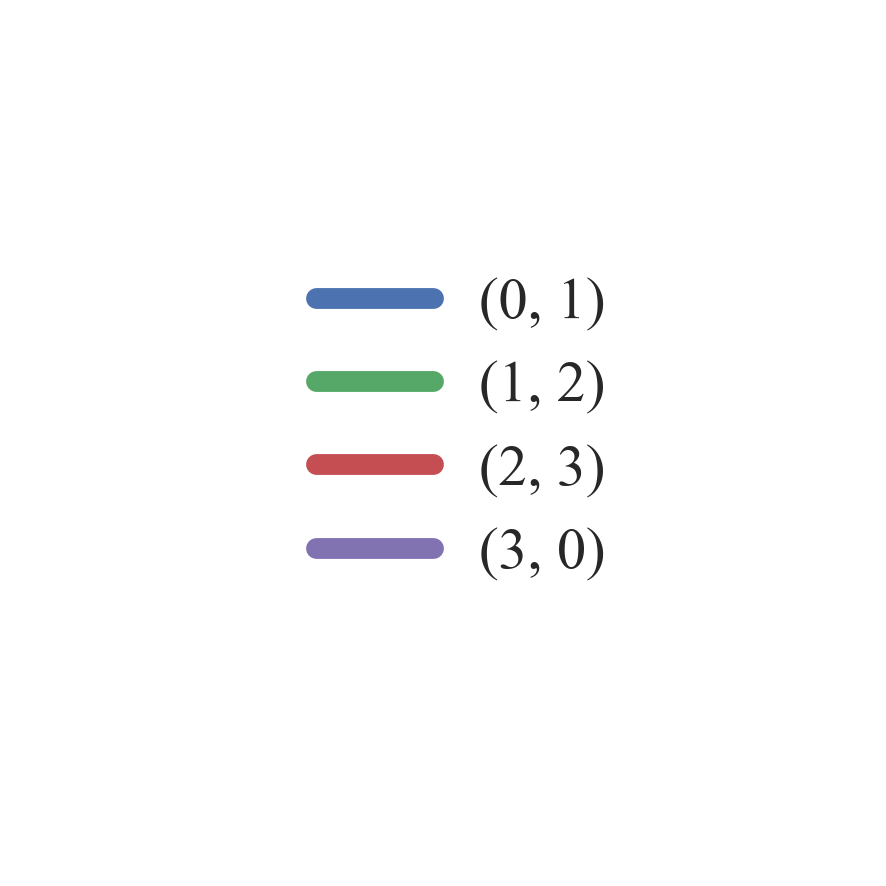
\includegraphics[width=0.4\linewidth,keepaspectratio,trim={0 3cm 0 2cm},clip]{./simulation/cycle/cycle_4_legend.png}\label{fig:cycle_4_legend}}
			\newline
			\subfloat[][]{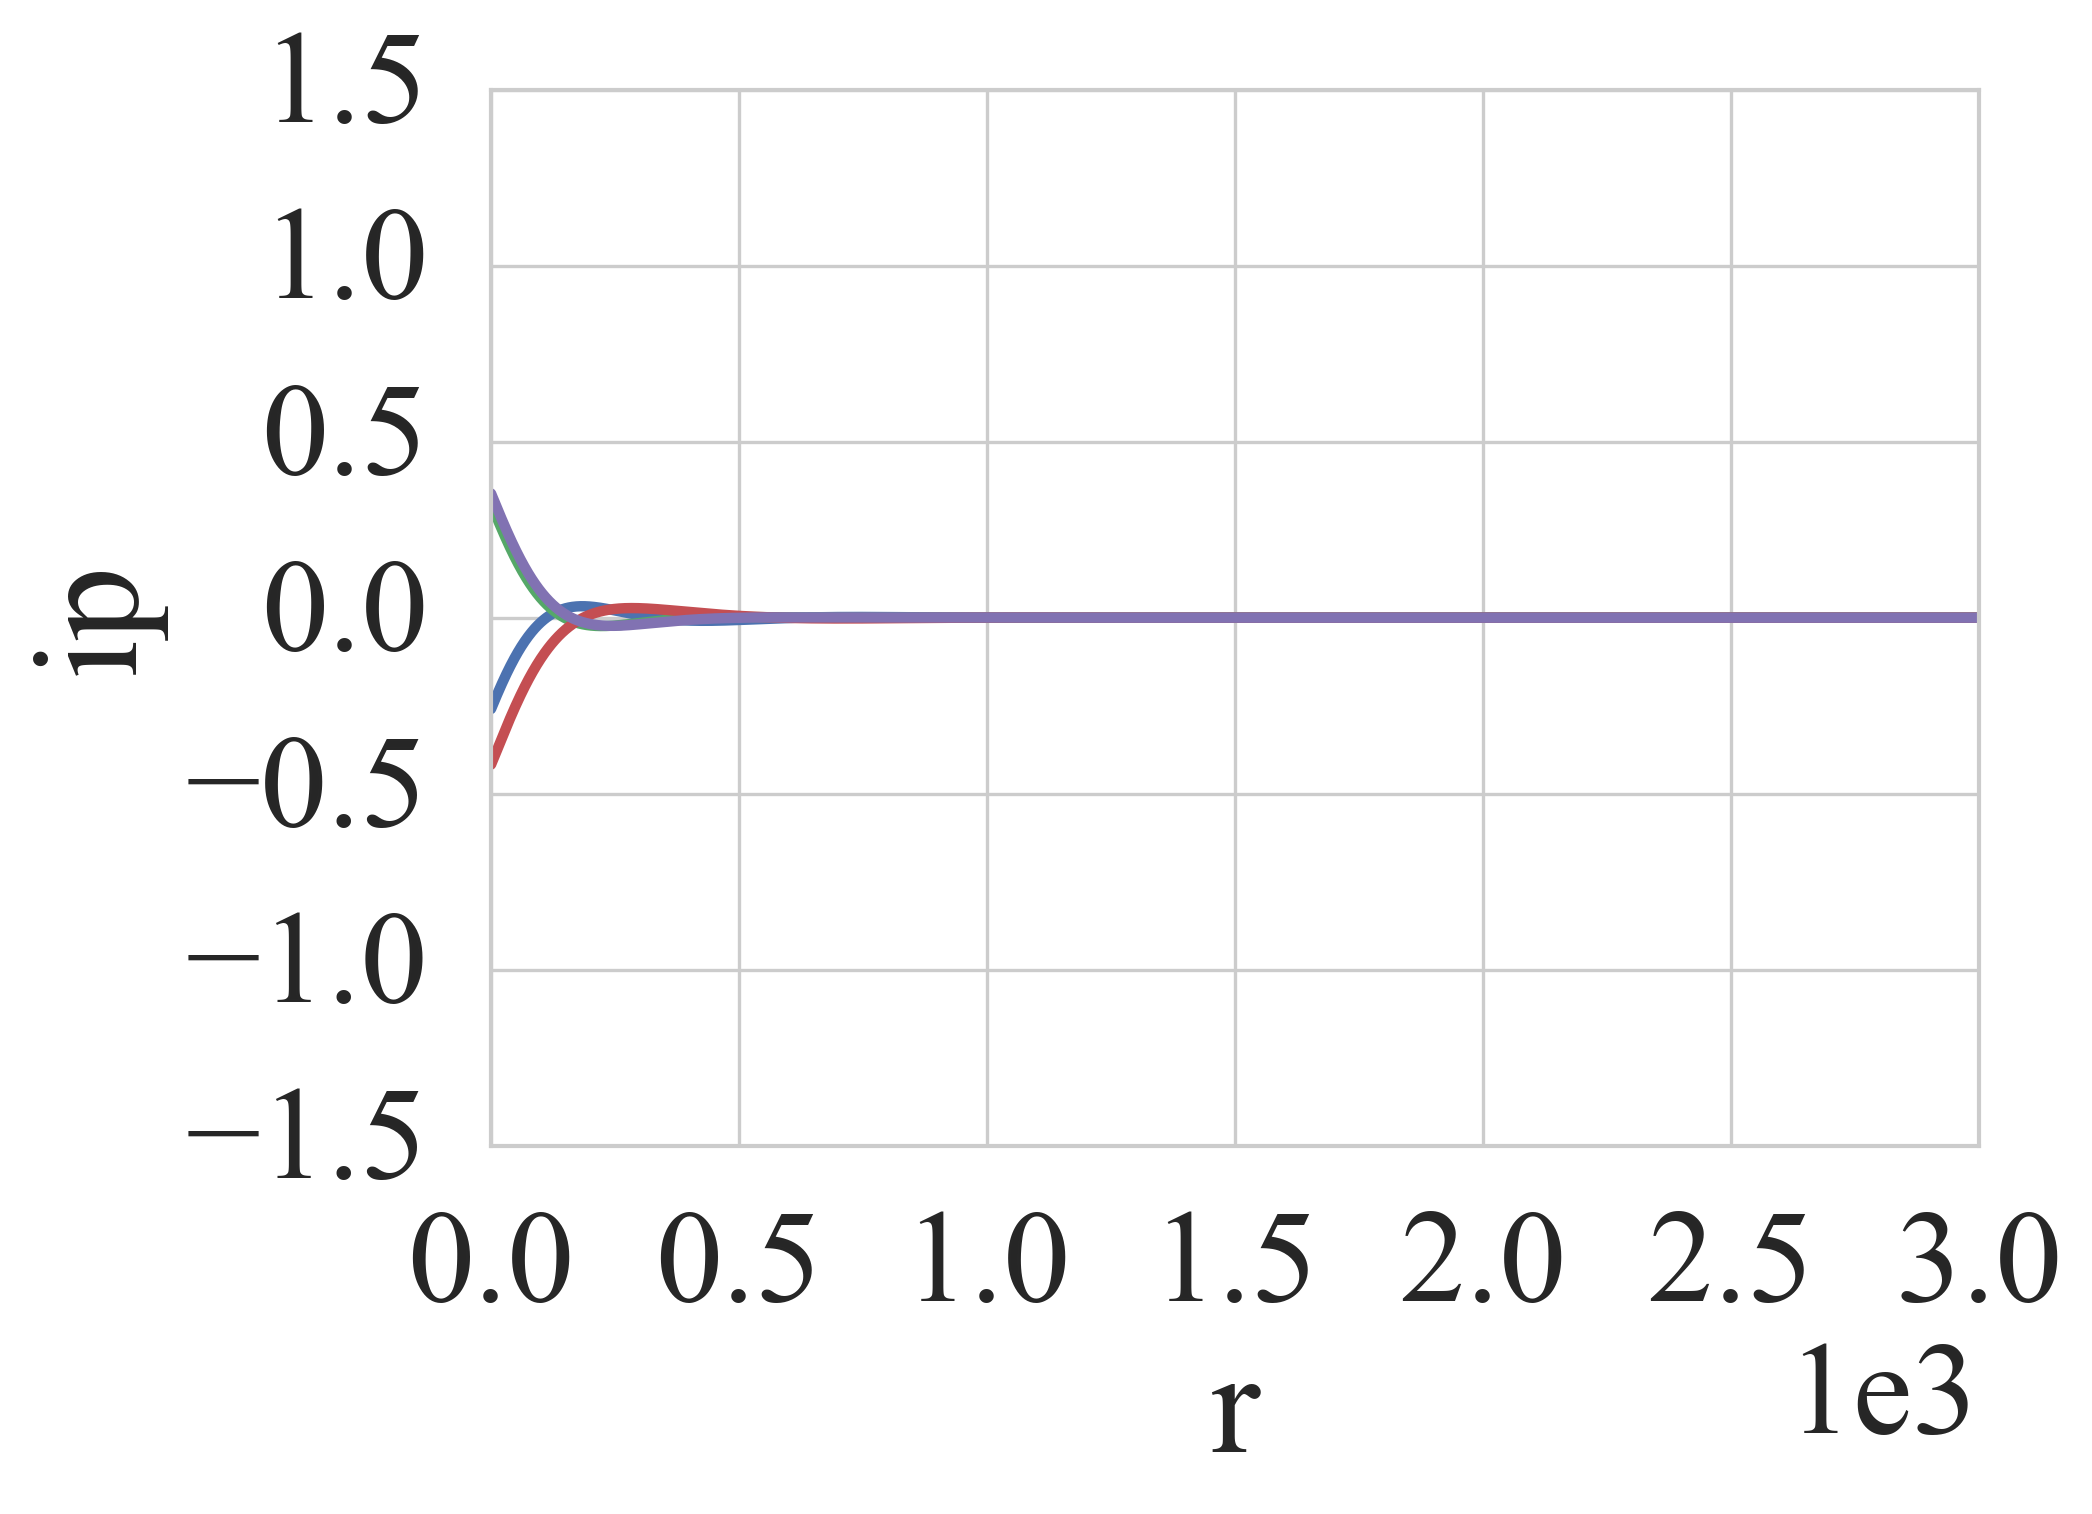
\includegraphics[width=0.4\linewidth,keepaspectratio]{./simulation/cycle/cycle_4_ip_zero.png}\label{fig:cycle_4_ip_zero}}\qquad
			\subfloat[][]{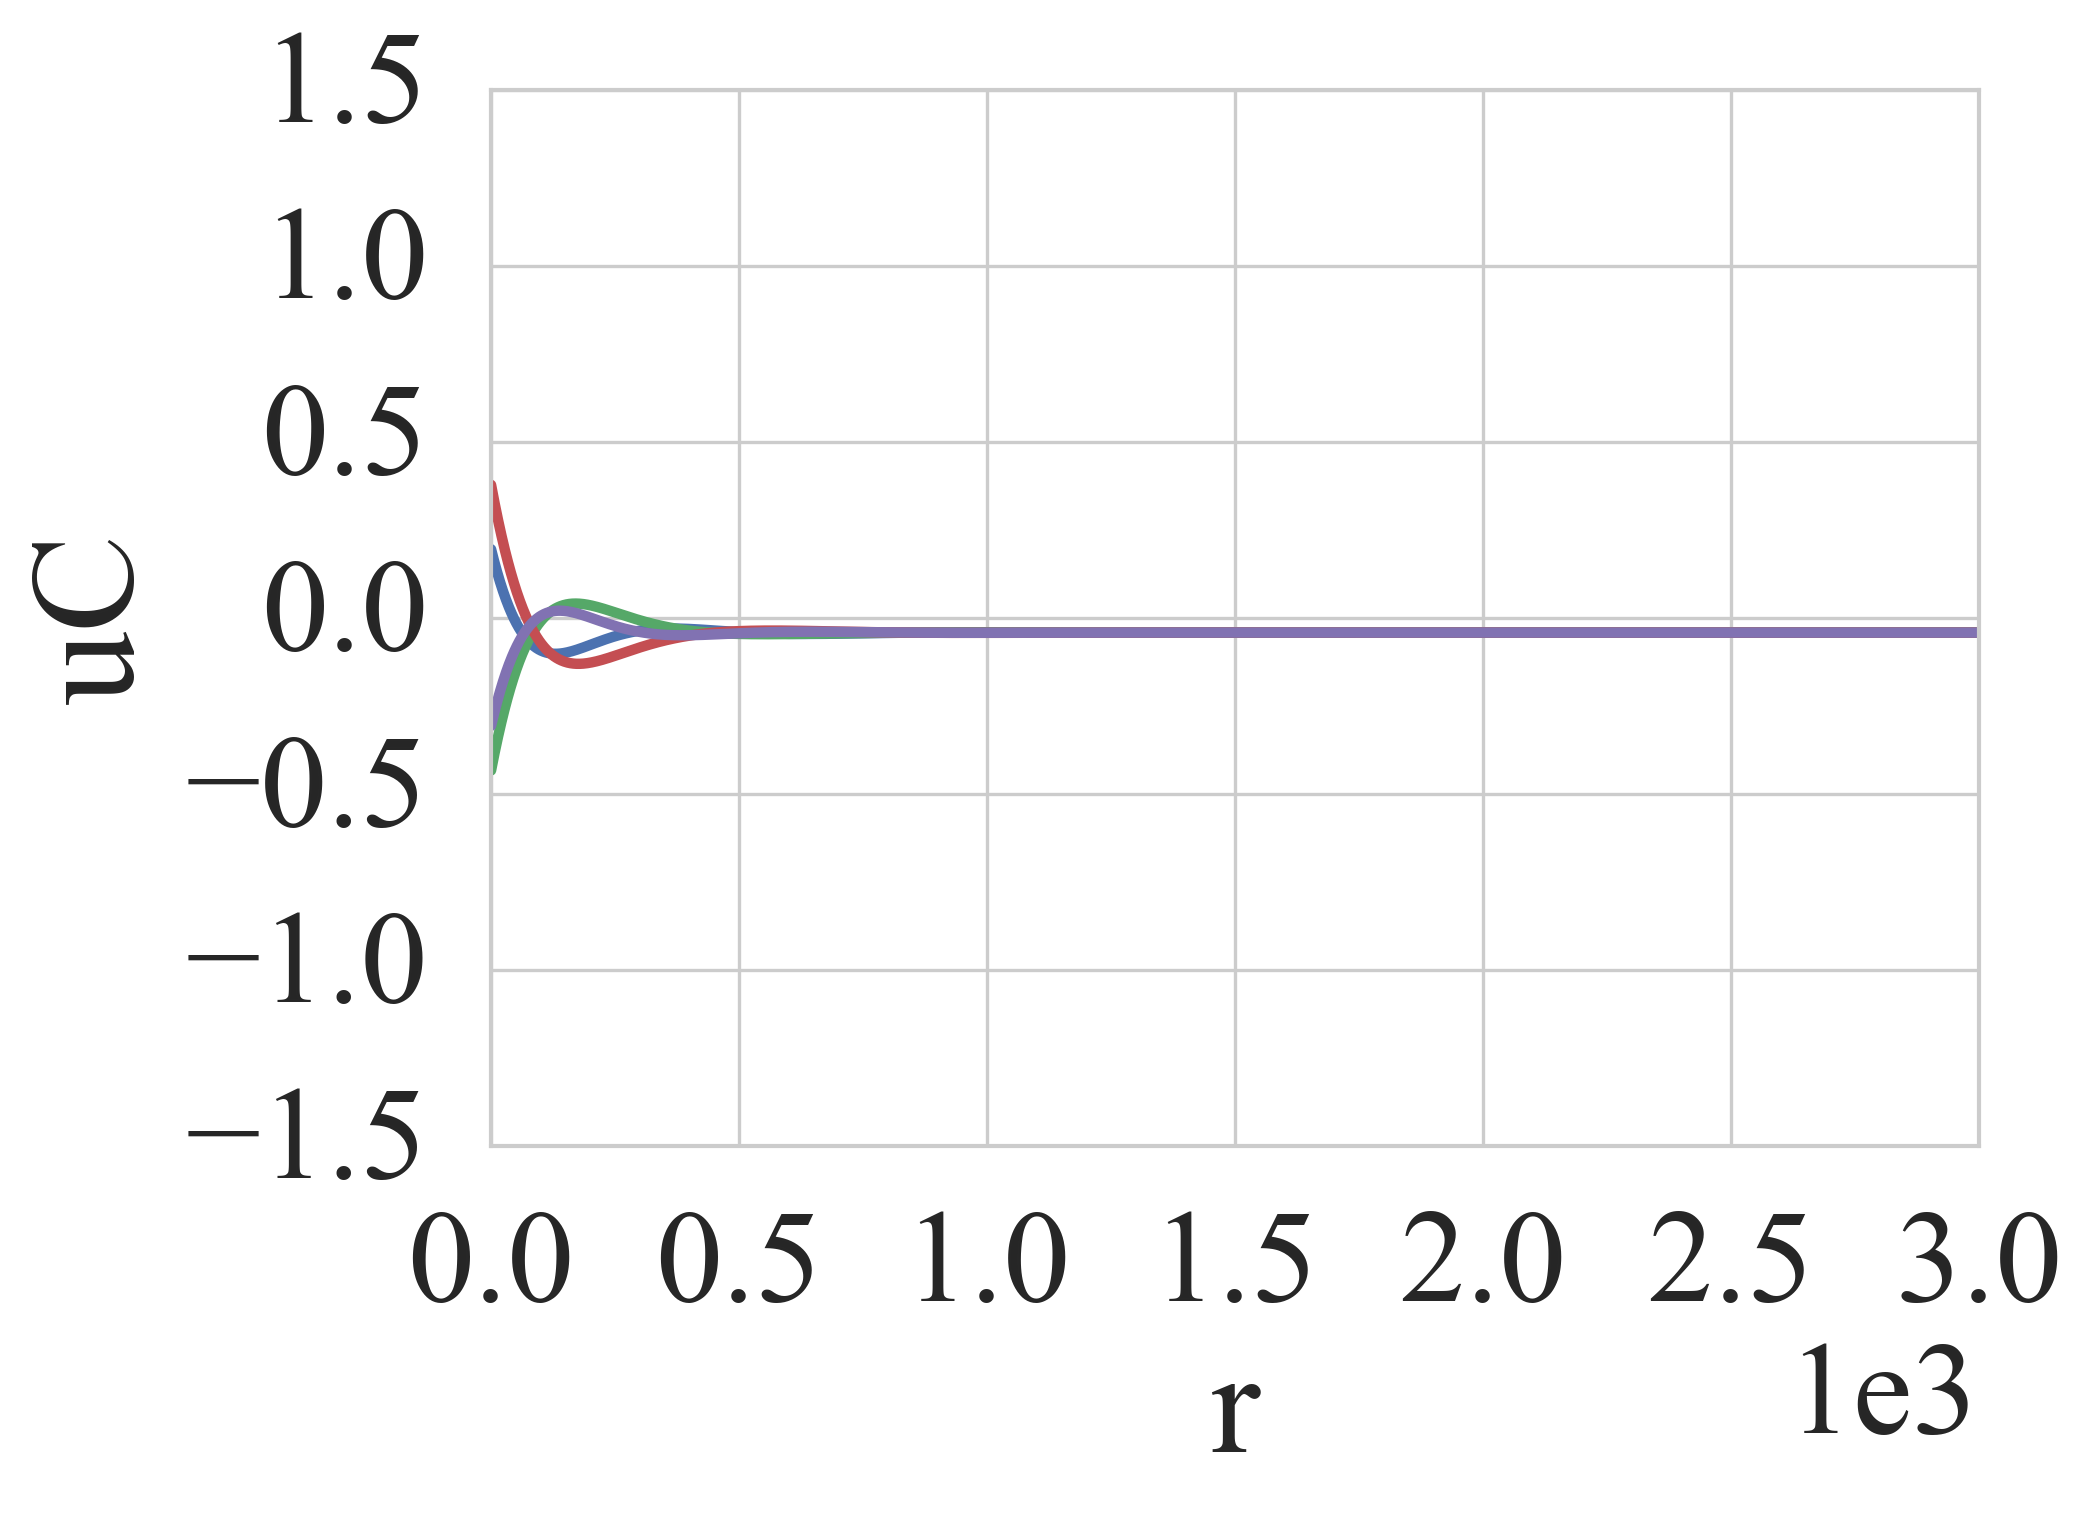
\includegraphics[width=0.4\linewidth,keepaspectratio]{./simulation/cycle/cycle_4_uC_zero.png}\label{fig:cycle_4_uC_zero}}
			\newline
			\subfloat[][]{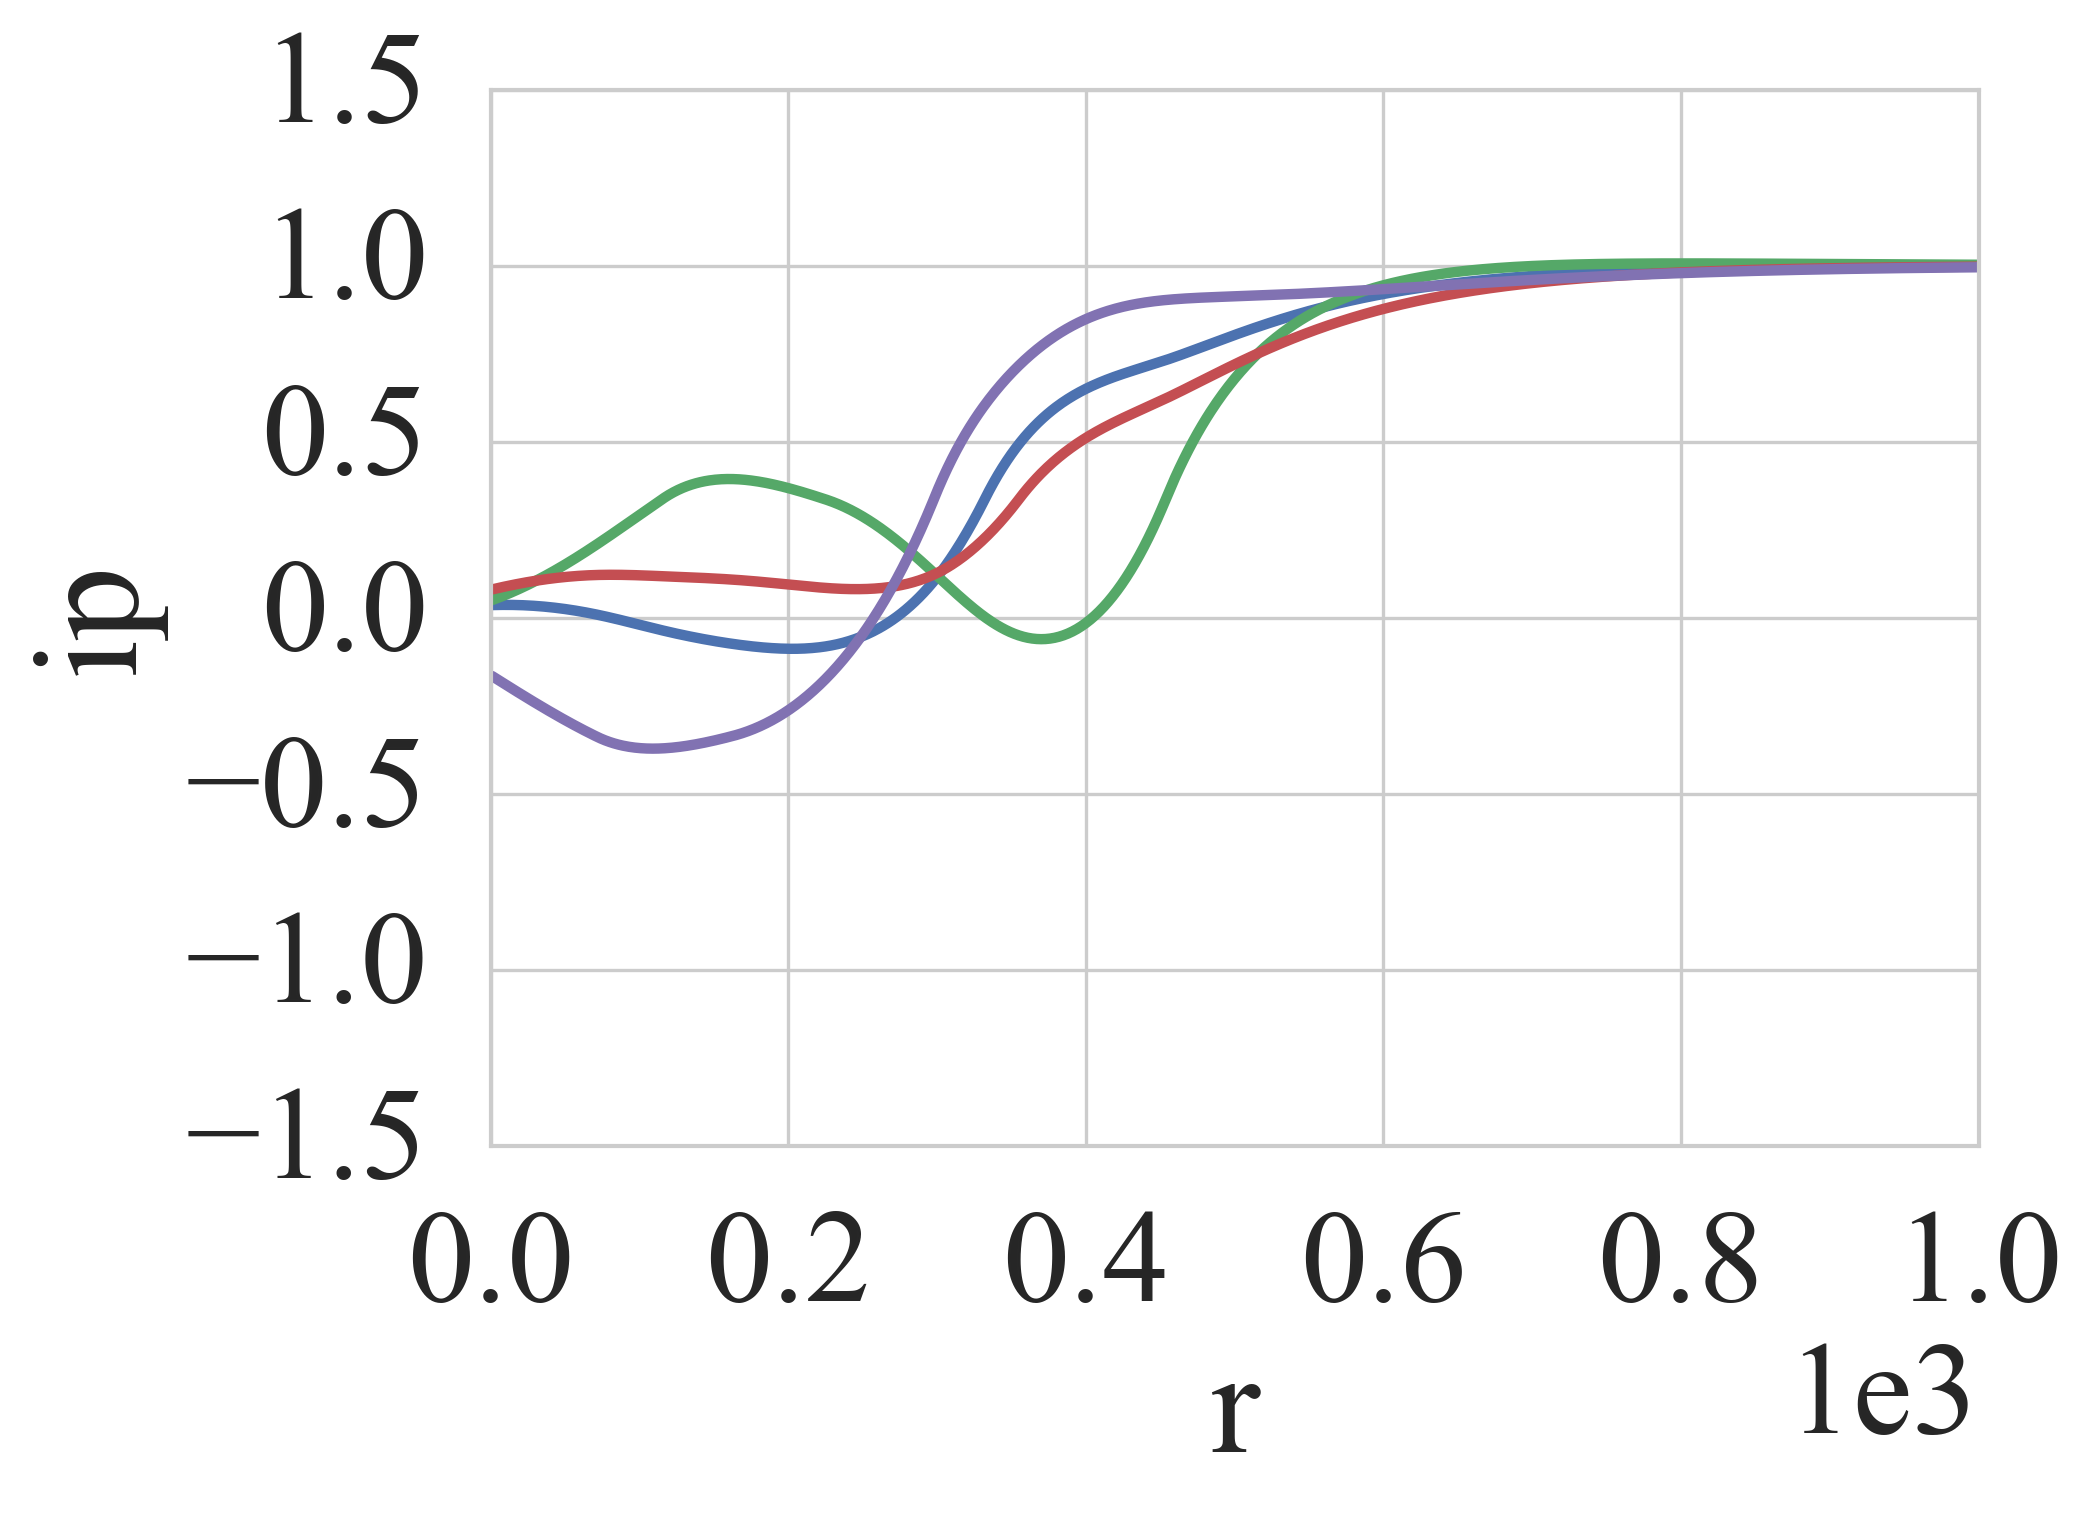
\includegraphics[width=0.4\linewidth,keepaspectratio]{./simulation/cycle/cycle_4_ip_positive.png}\label{fig:cycle_4_ip_positive}}\qquad
			\subfloat[][]{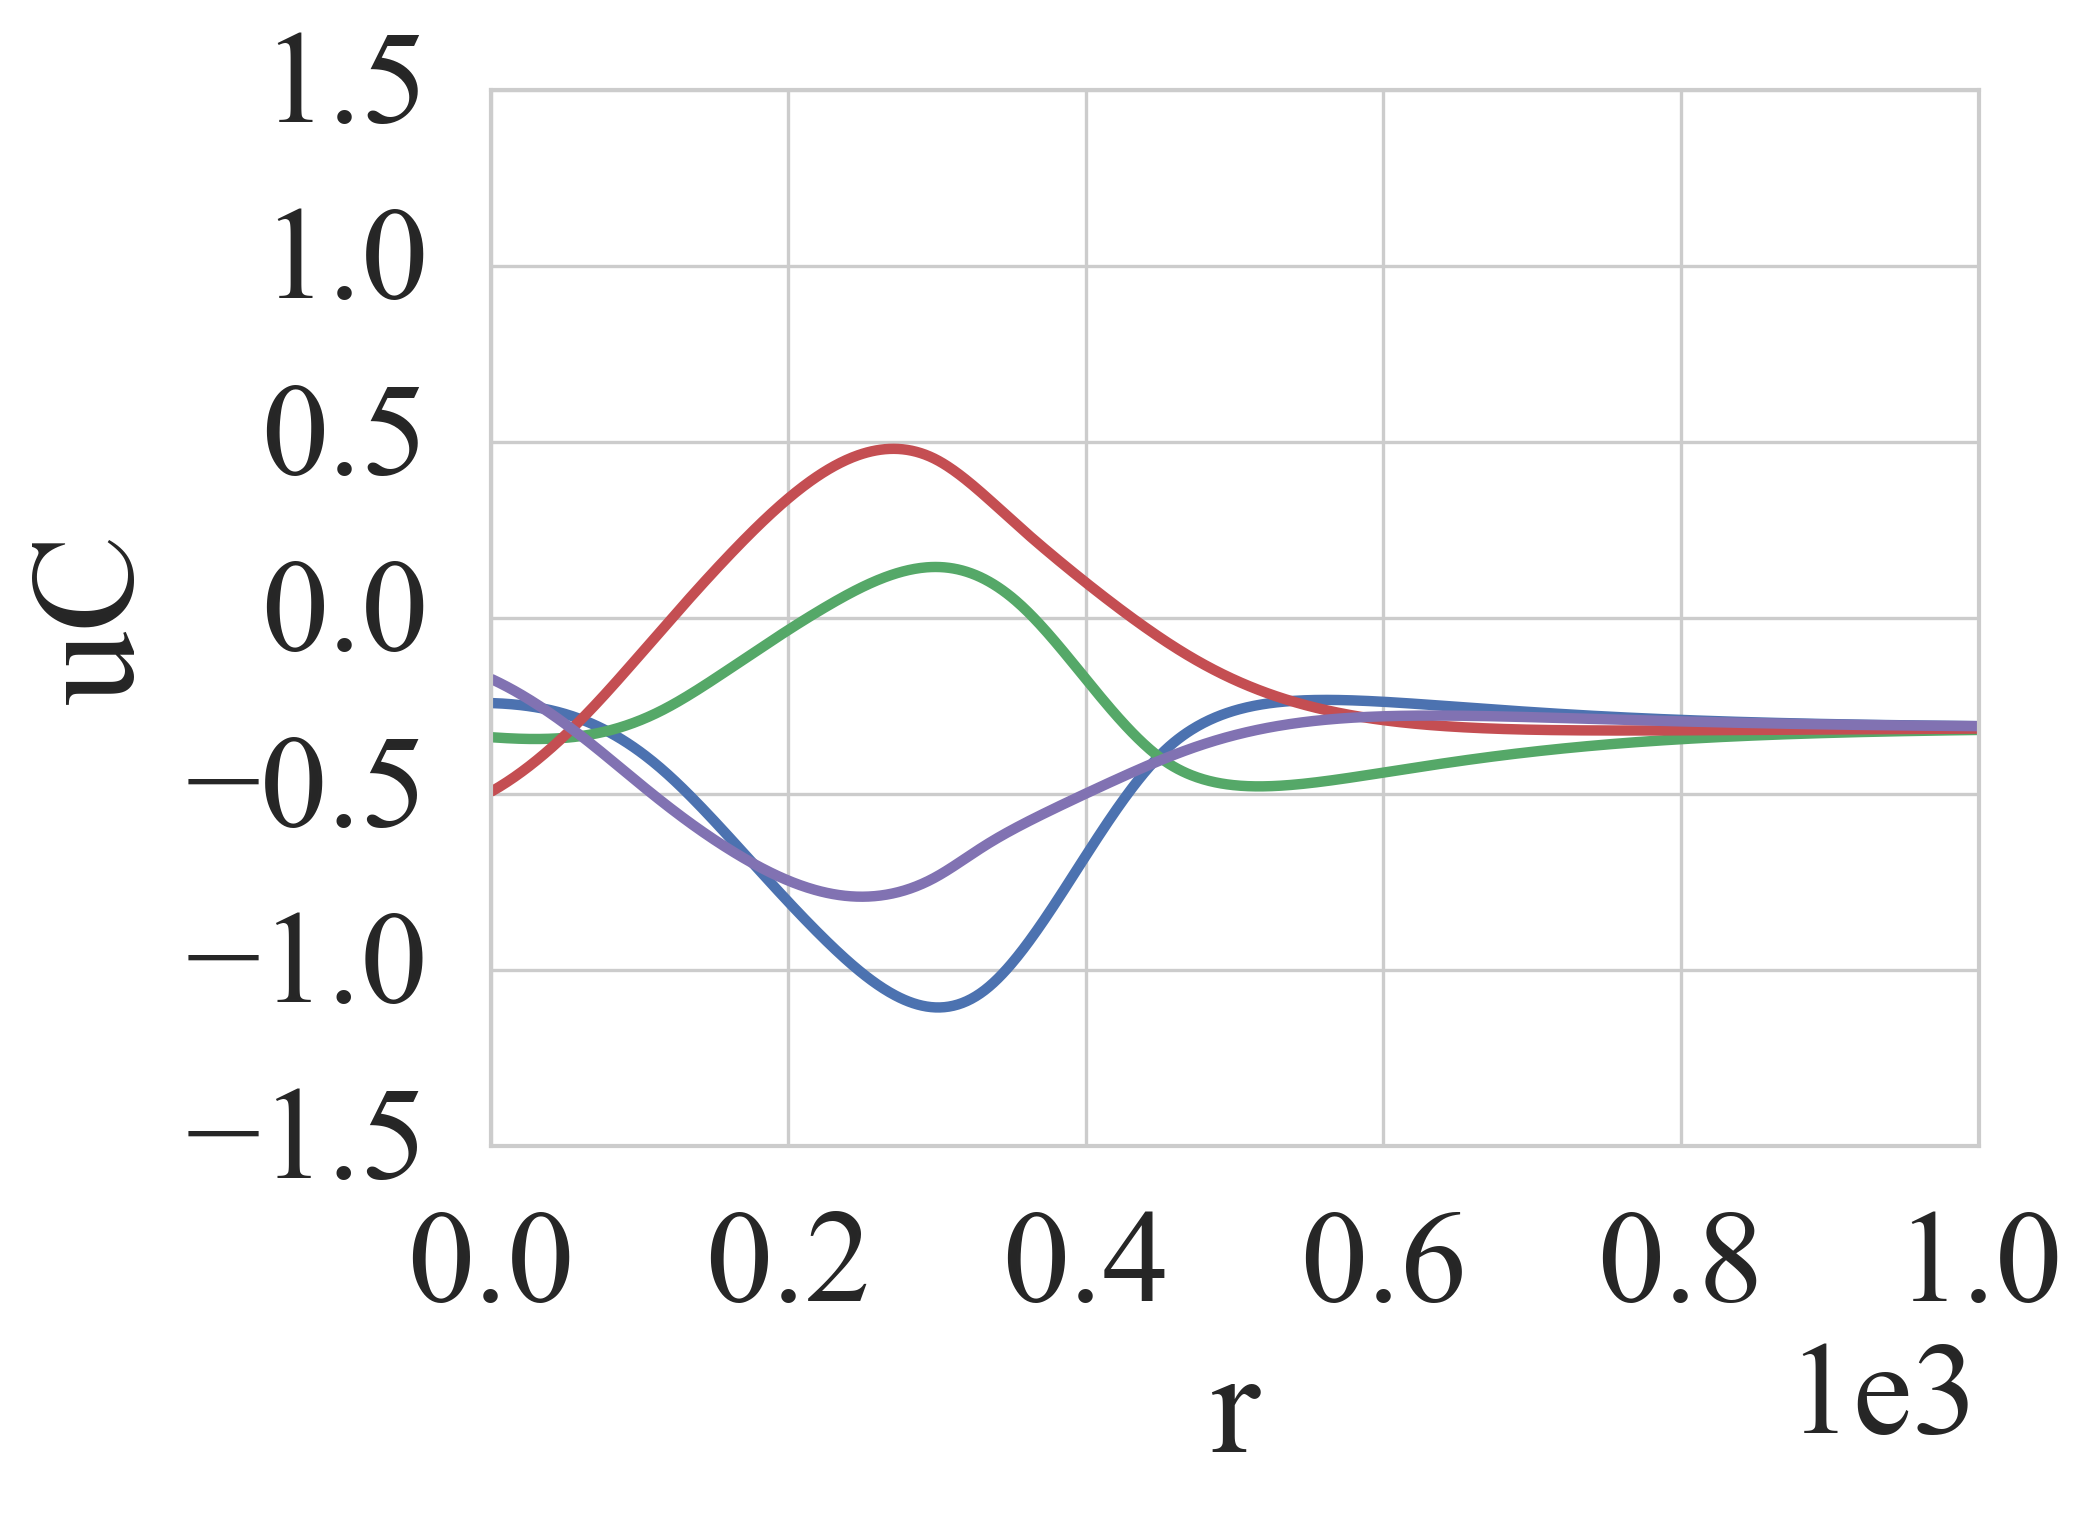
\includegraphics[width=0.4\linewidth,keepaspectratio]{./simulation/cycle/cycle_4_uC_positive.png}\label{fig:cycle_4_uC_positive}}
			\newline
			\subfloat[][]{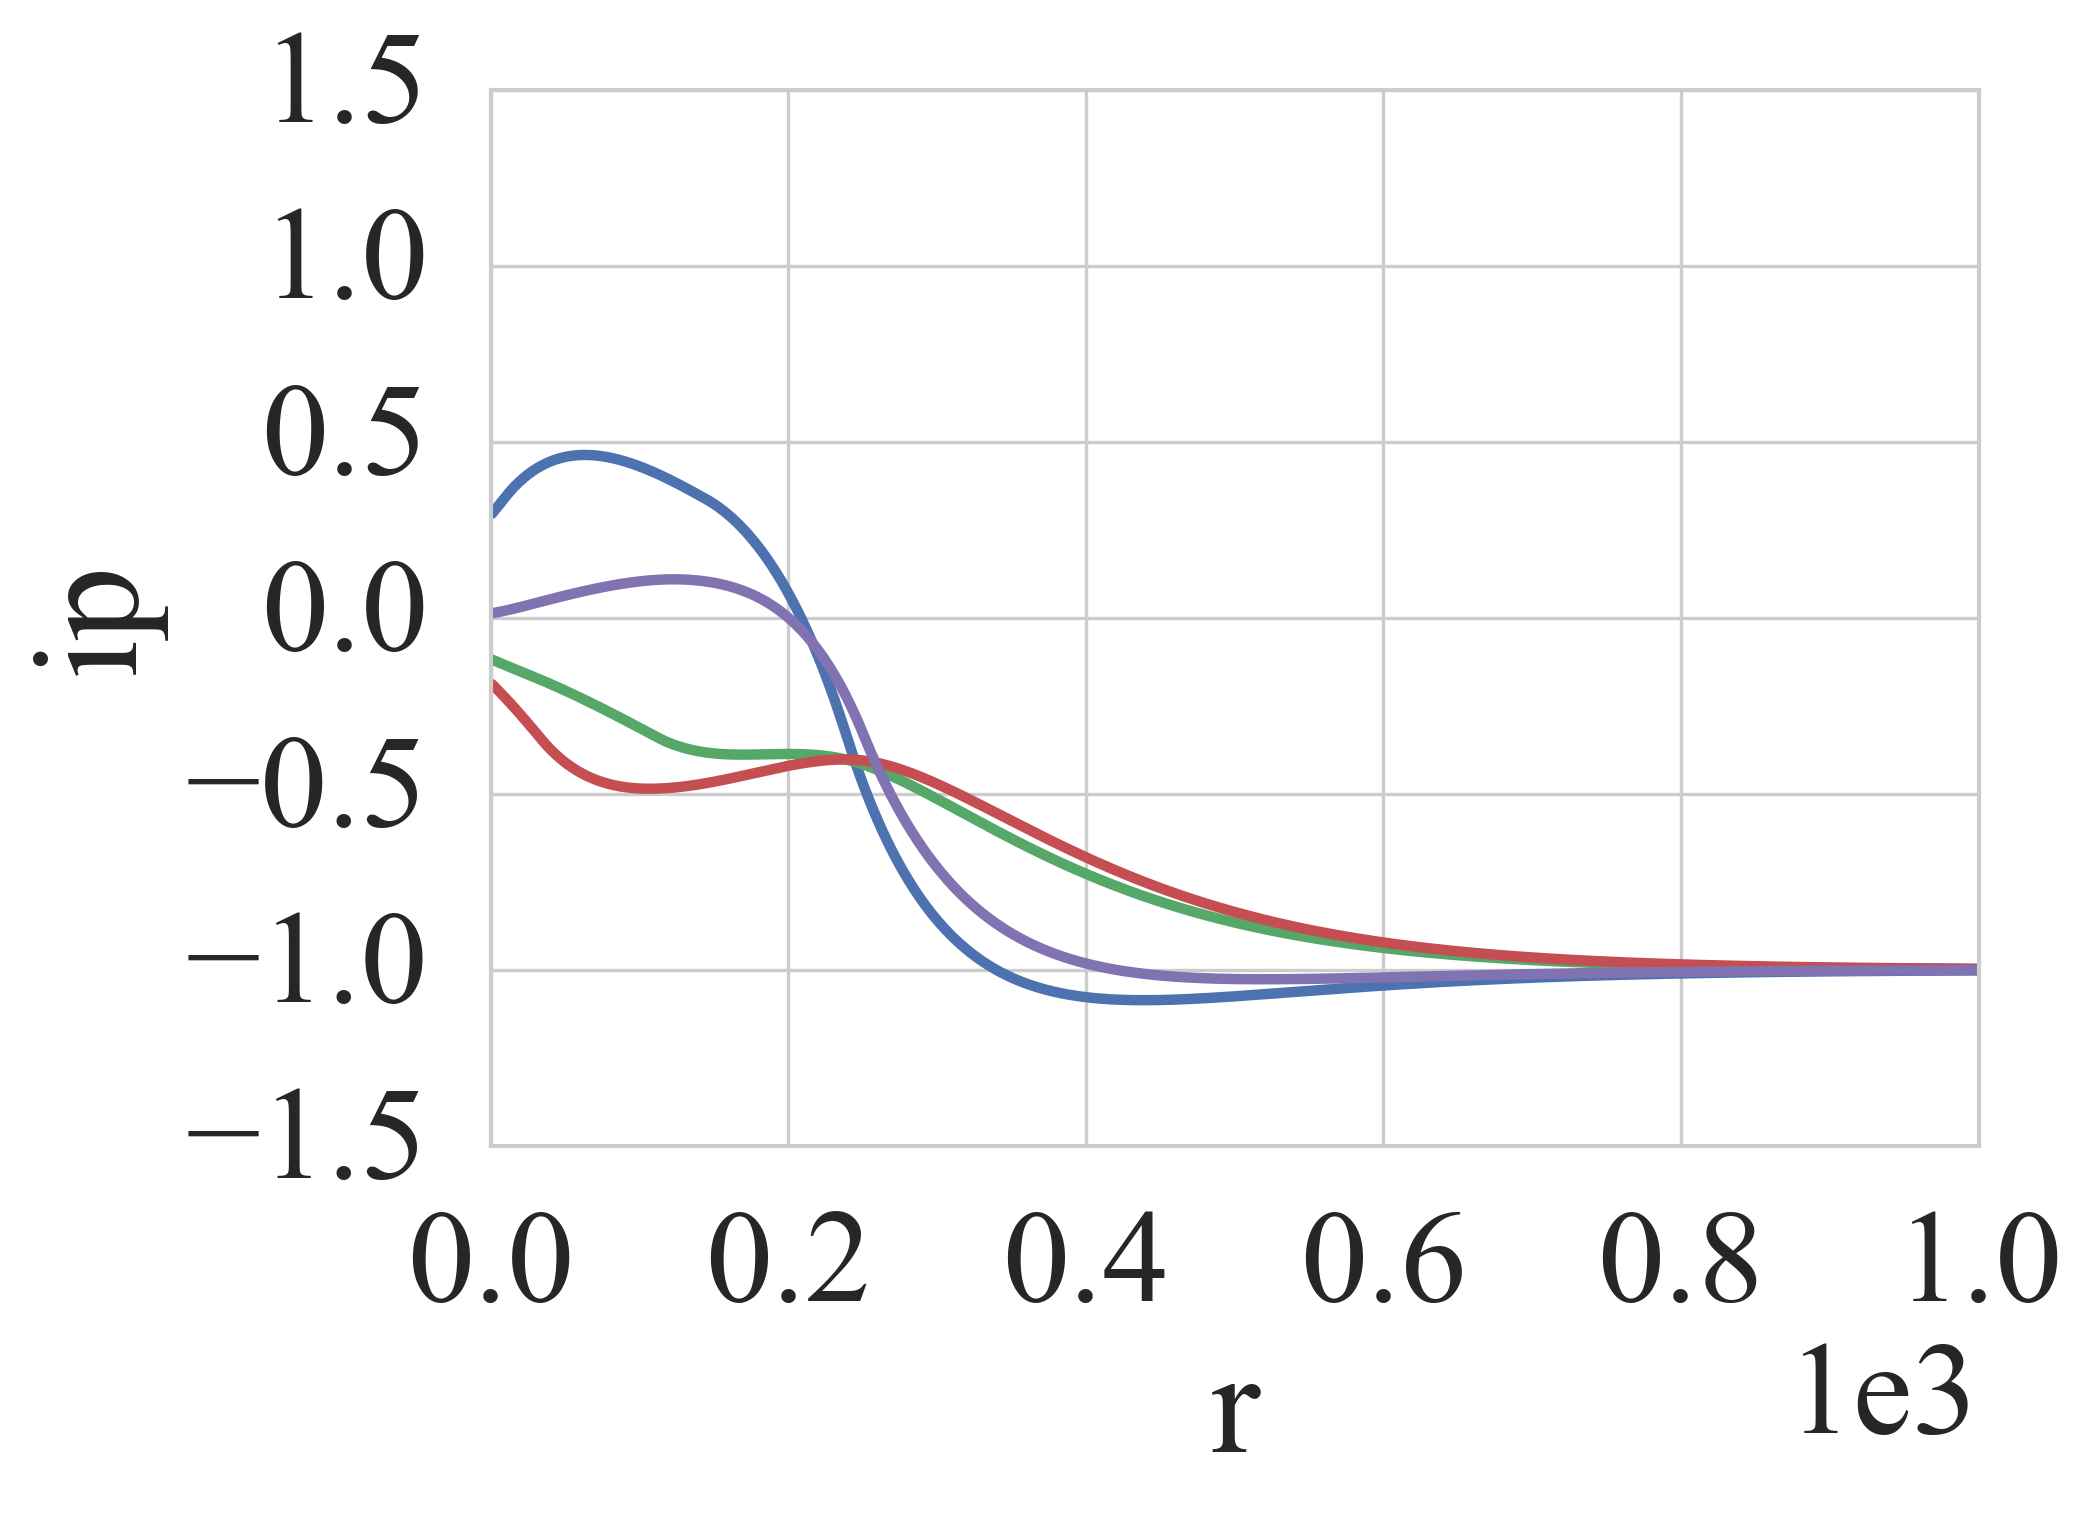
\includegraphics[width=0.4\linewidth,keepaspectratio]{./simulation/cycle/cycle_4_ip_negative.png}\label{fig:cycle_4_ip_negative}}\qquad
			\subfloat[][]{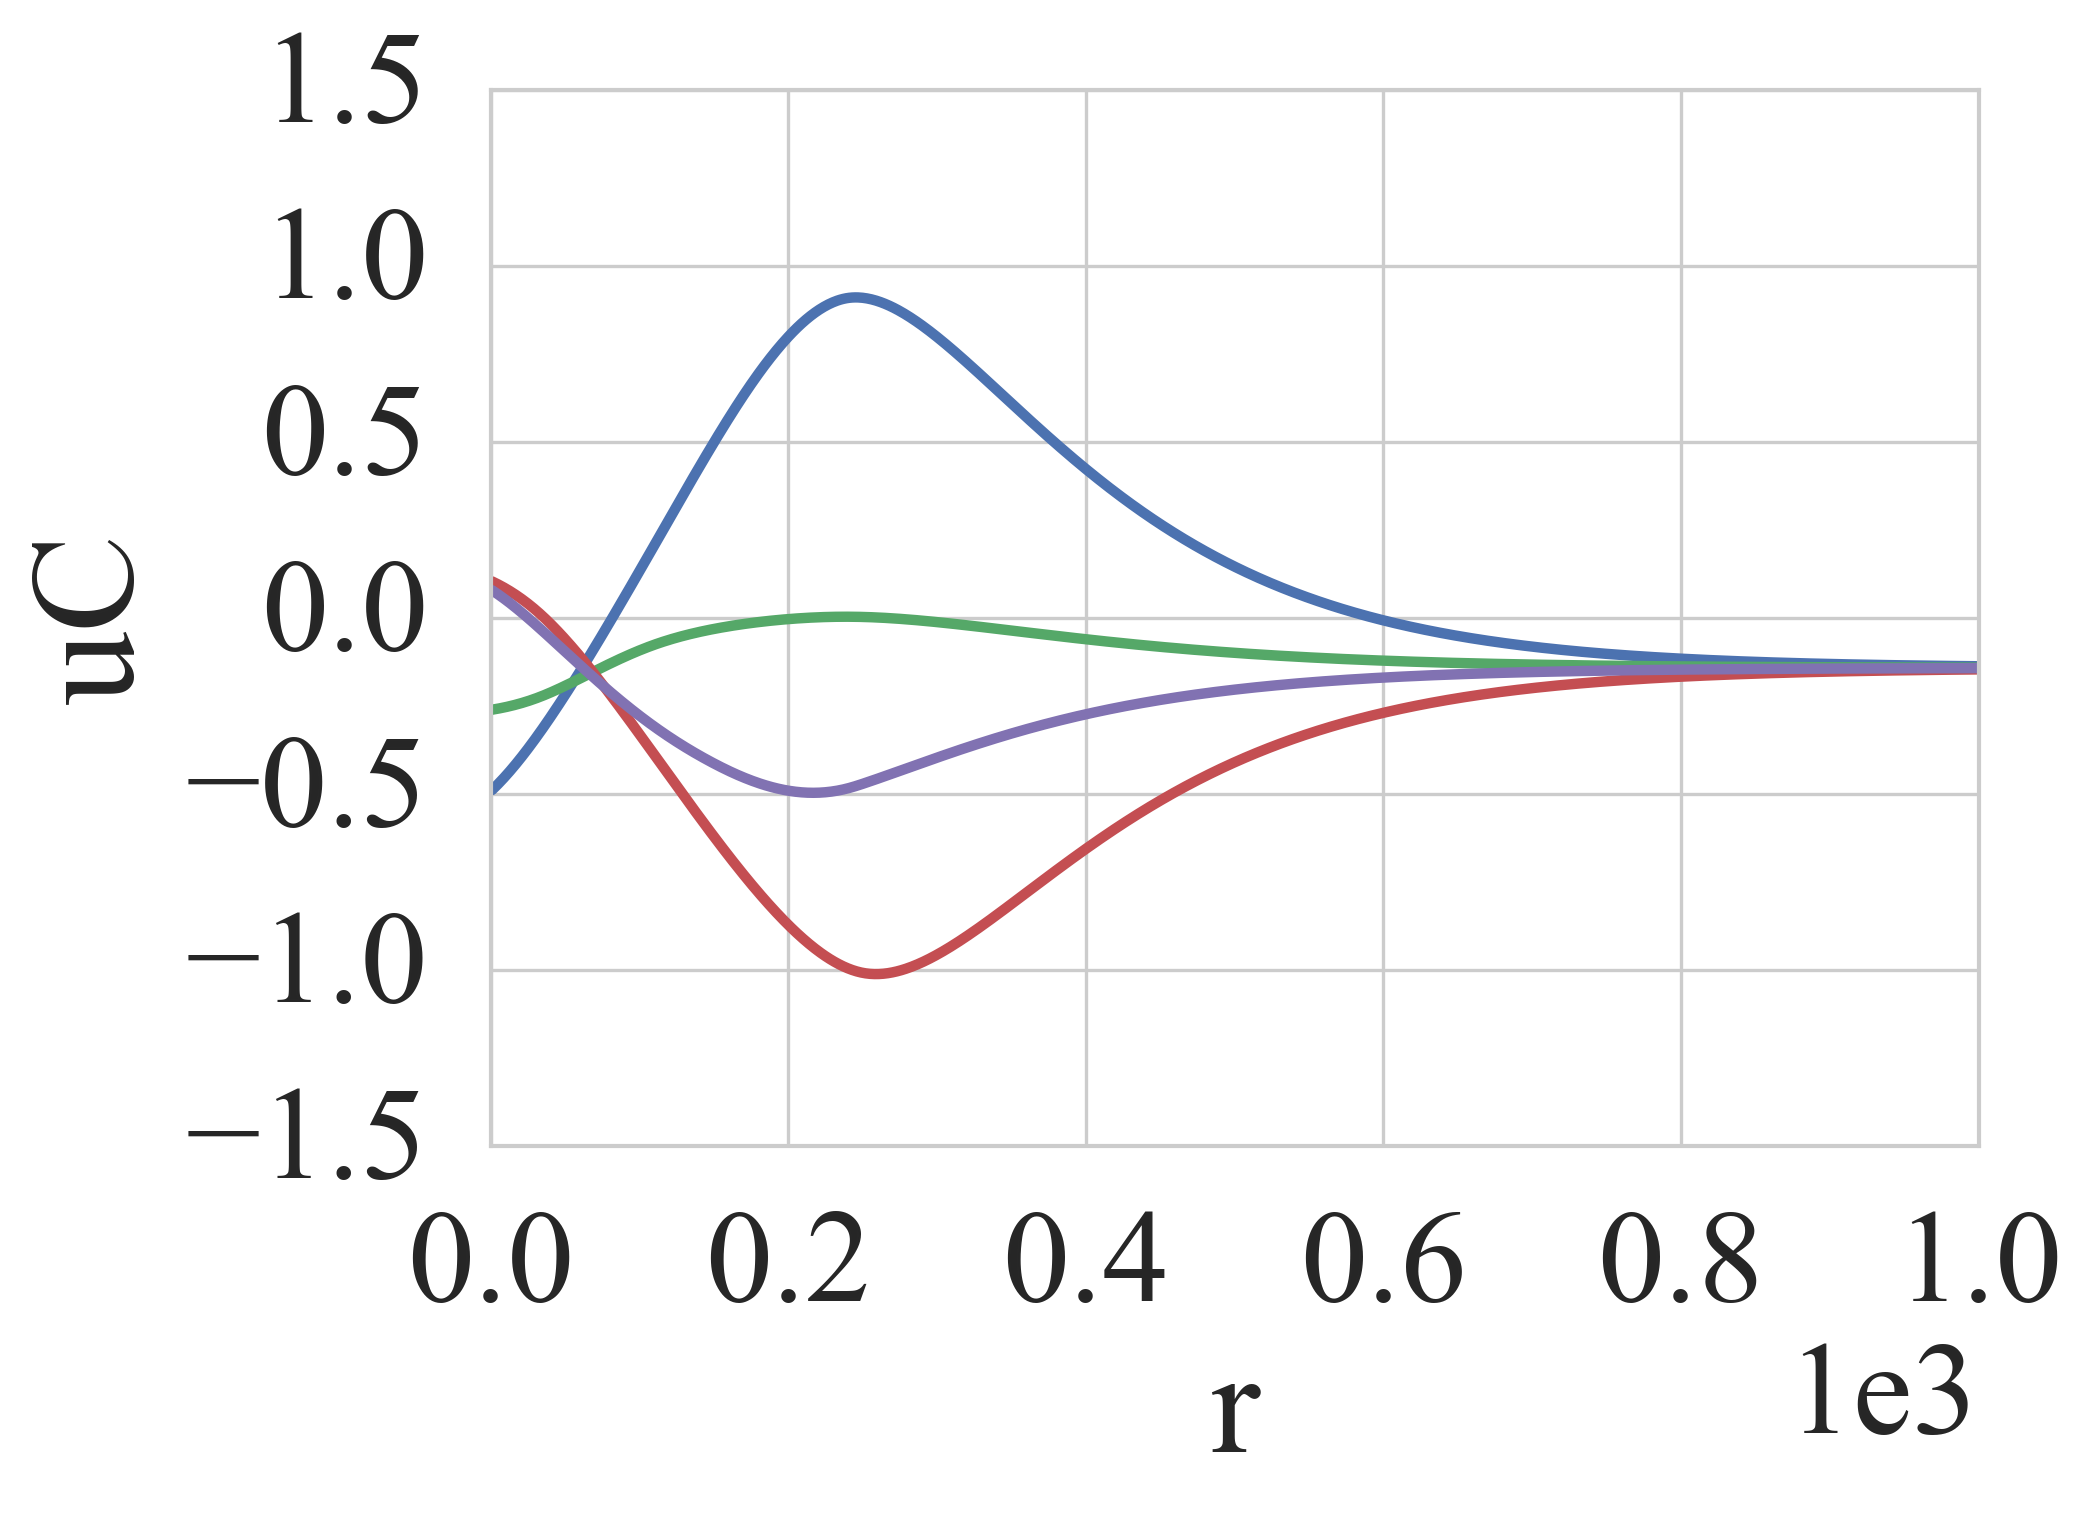
\includegraphics[width=0.4\linewidth,keepaspectratio]{./simulation/cycle/cycle_4_uC_negative.png}\label{fig:cycle_4_uC_negative}}
			
			\caption[Simulation - Cycles]{Cycle of $4$ \Pes.}
			\label{fig:cycle}
		\end{figure}

		\FloatBarrier

	\subsection{Diamond of Physarum Elements}

		The graph we investigate next is the so-called diamond graph depicted in \Fref{fig:diamond_graph}. This topology is also widely known under the name of Wheatstone graph or Wheatstone bridge. It consists of a $4$-cycle with an additional ``bridge'' edge $(2,0)$ added. Again \Fref{fig:diamond_graph_legend} defines a color coding which serves as a legend for the remaining plots of \Fref{fig:diamond}. We show the results of three distinct runs of the simulation.

		Similar to the $4$-cycle explored previously, we investigate several scenarios. In all of them the capacitor voltages $u_{C,e}(t)$ quickly converge, see \Fref{fig:diamond_uC_symmetric_positive}, \Fref{fig:diamond_uC_symmetric_negative} and \Fref{fig:diamond_uC_asymmetric_positive}. However, due to the additional edge introduced to the \Pn, edges do not converge to the same values anymore but split up in three distinct groups. The first group is formed by edges $(0,1)$ and $(1,2)$. The second group are edges $(2,3)$ and $(3,0)$. And the last group is the bridge edge $(2,0)$. Note that in all scenarios the voltages show that the first two groups are symmetric around the value the center edge converges to. Although the capacitor voltages show identical behavior, very different currents can be accommodated.

		\Fref{fig:diamond_ip_symmetric_positive} shows a scenario, where $1.5$ units of current flow through the center edge to split evenly at node $0$. The split flow then circles back to node $2$ showing appropriate signs and values. \Fref{fig:diamond_ip_symmetric_negative} shows the same situation but with the flow on the center edge reversed. Naturally, there is no reason to assume that flow must split up symmetrically. \Fref{fig:diamond_ip_asymmetric_positive} shows one of many possible unbalanced scenarios. As in the case of the $4$-cycle, we do not know the details of the splitting process nor its dependence on initial conditions at this point.

		\begin{figure}
			\centering
			\subfloat[][]{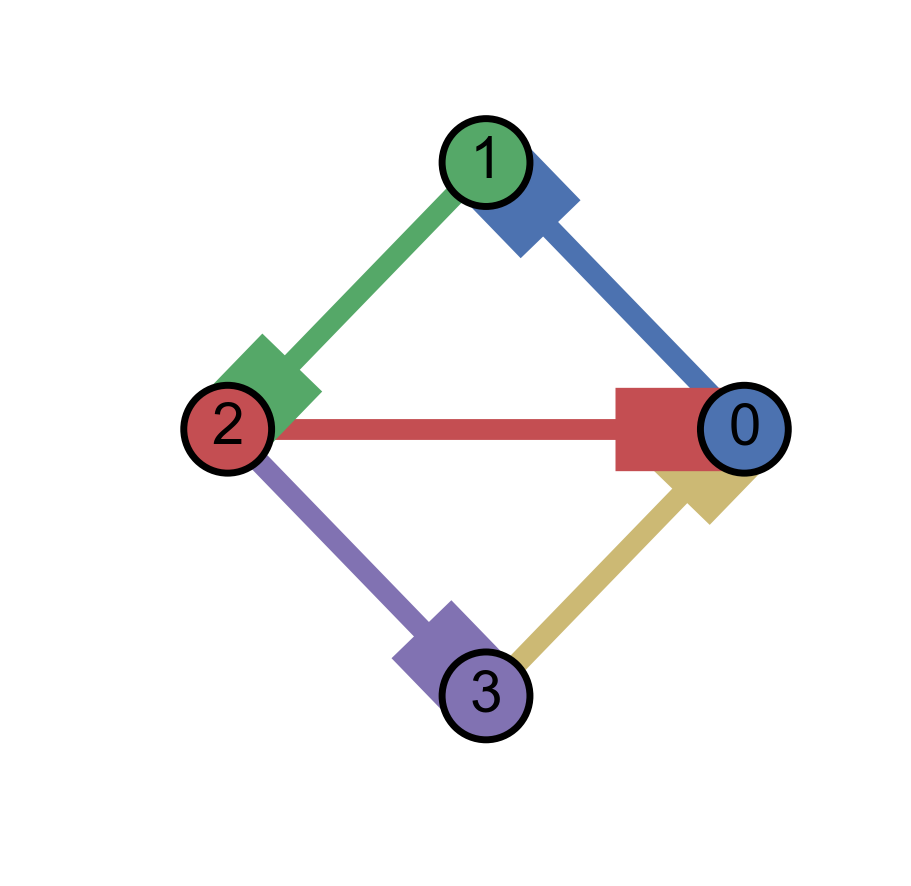
\includegraphics[width=0.4\linewidth,keepaspectratio,trim={0 3cm 0 2cm},clip]{./simulation/diamond/diamond.png}\label{fig:diamond_graph}}\qquad
			\subfloat[][]{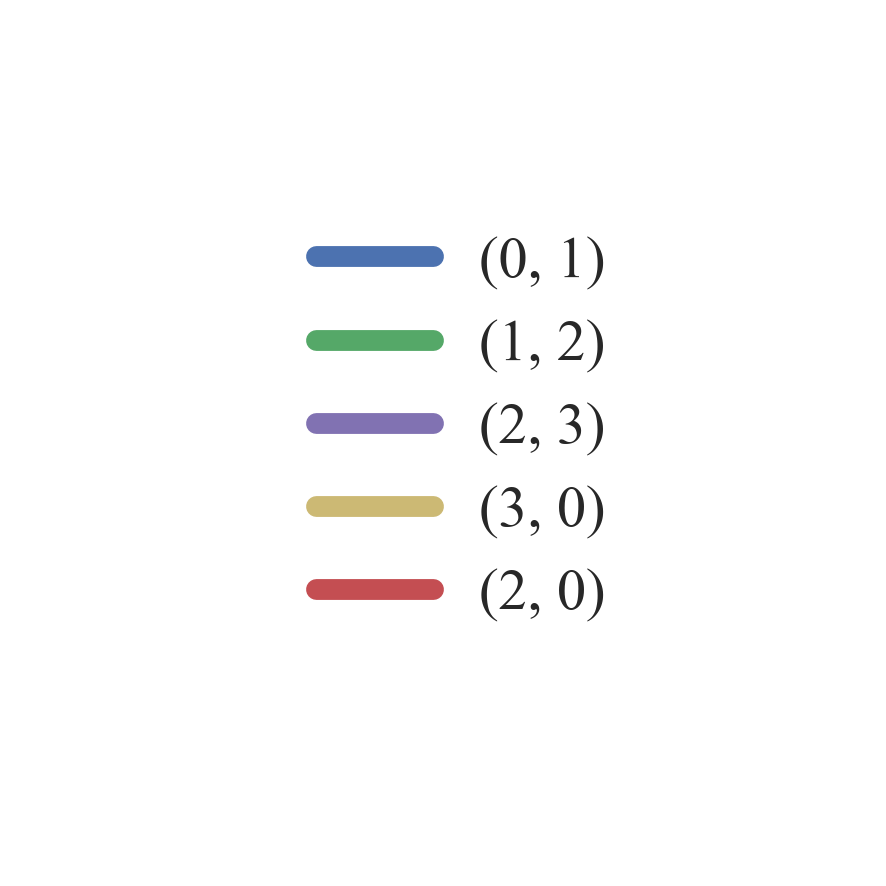
\includegraphics[width=0.4\linewidth,keepaspectratio,trim={0 3cm 0 2cm},clip]{./simulation/diamond/diamond_legend.png}\label{fig:diamond_graph_legend}}
			\newline
			\subfloat[][]{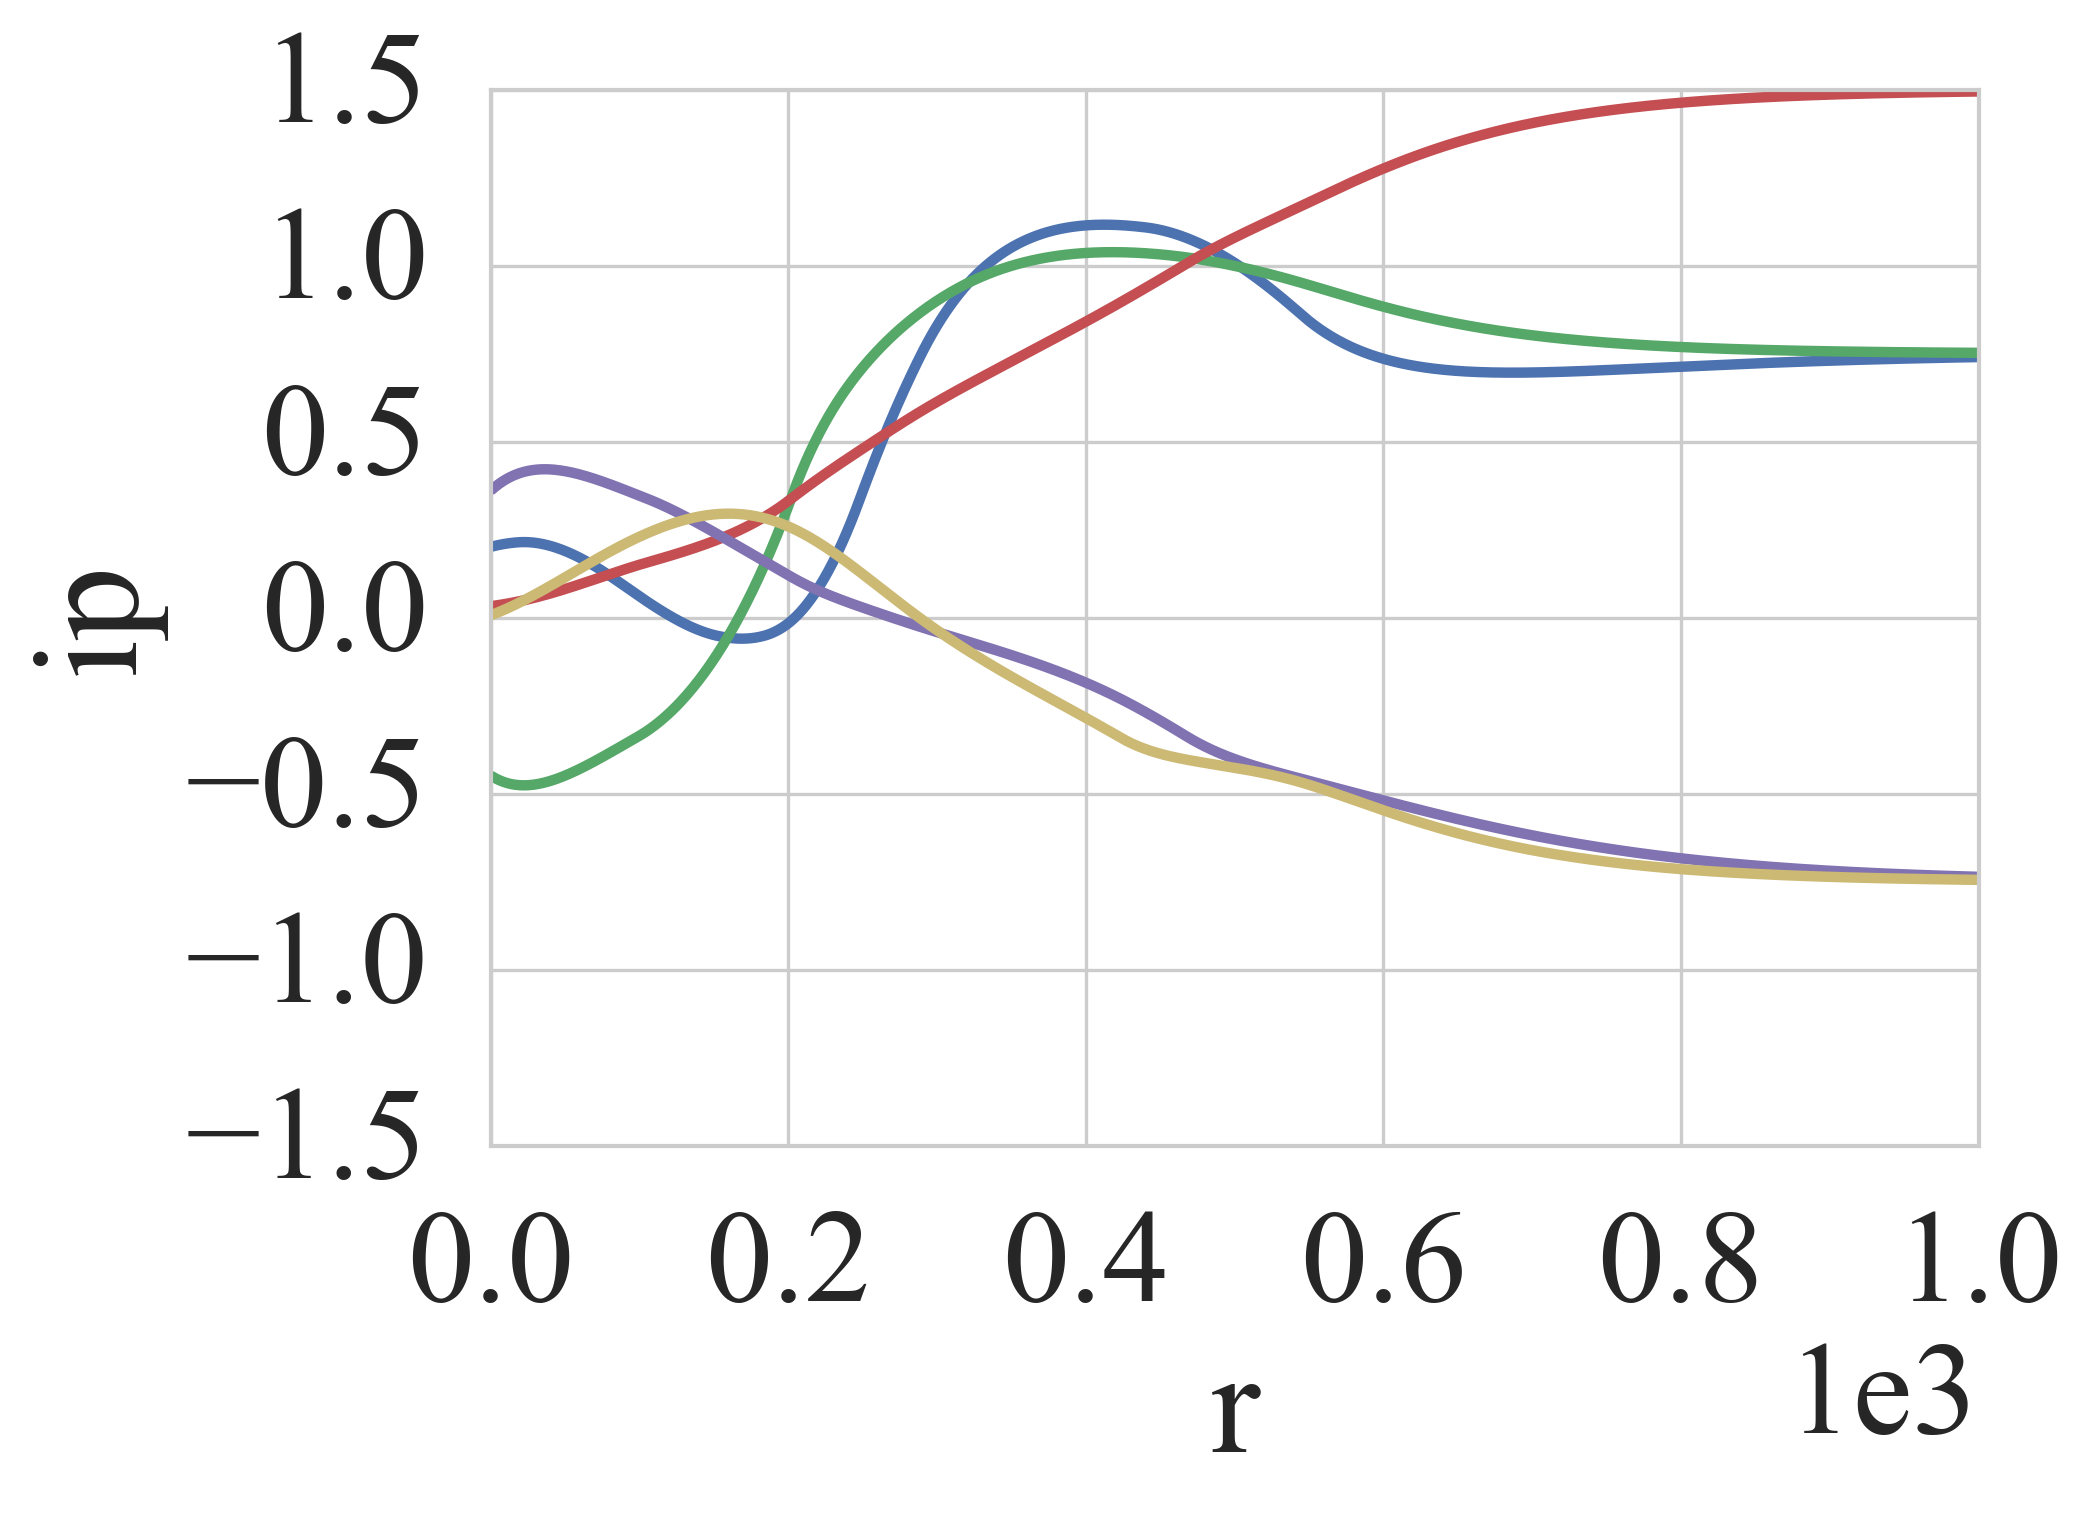
\includegraphics[width=0.4\linewidth,keepaspectratio]{./simulation/diamond/diamond_ip_symmetric_positive.png}\label{fig:diamond_ip_symmetric_positive}}\qquad
			\subfloat[][]{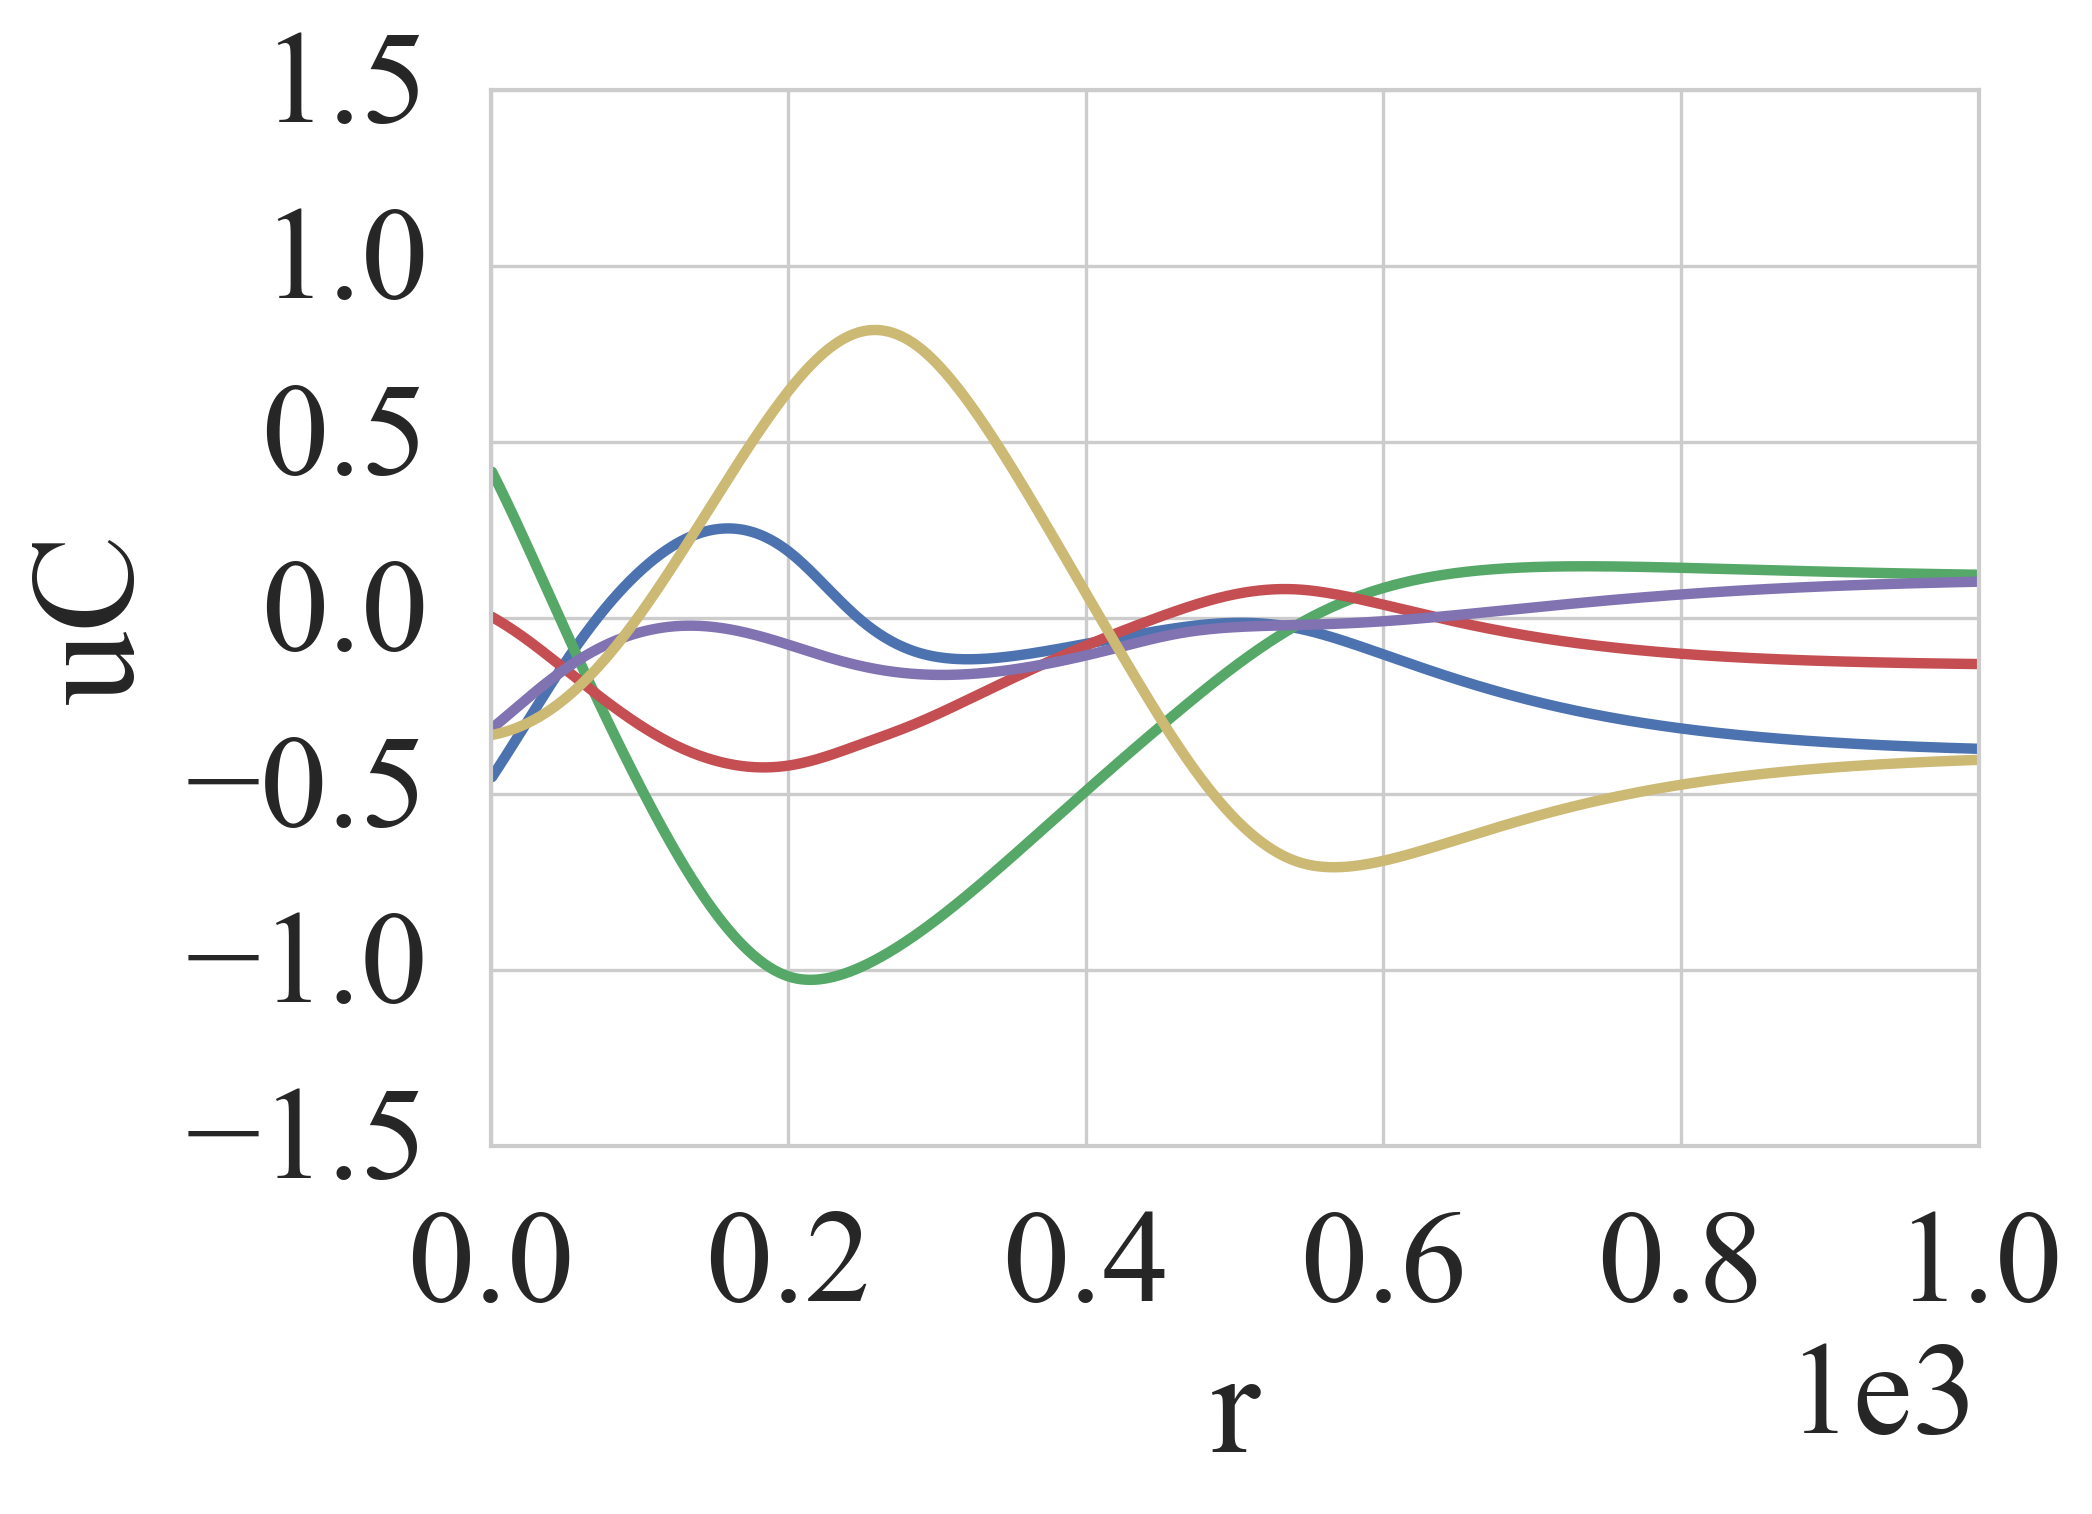
\includegraphics[width=0.4\linewidth,keepaspectratio]{./simulation/diamond/diamond_uC_symmetric_positive.png}\label{fig:diamond_uC_symmetric_positive}}
			\newline
			\subfloat[][]{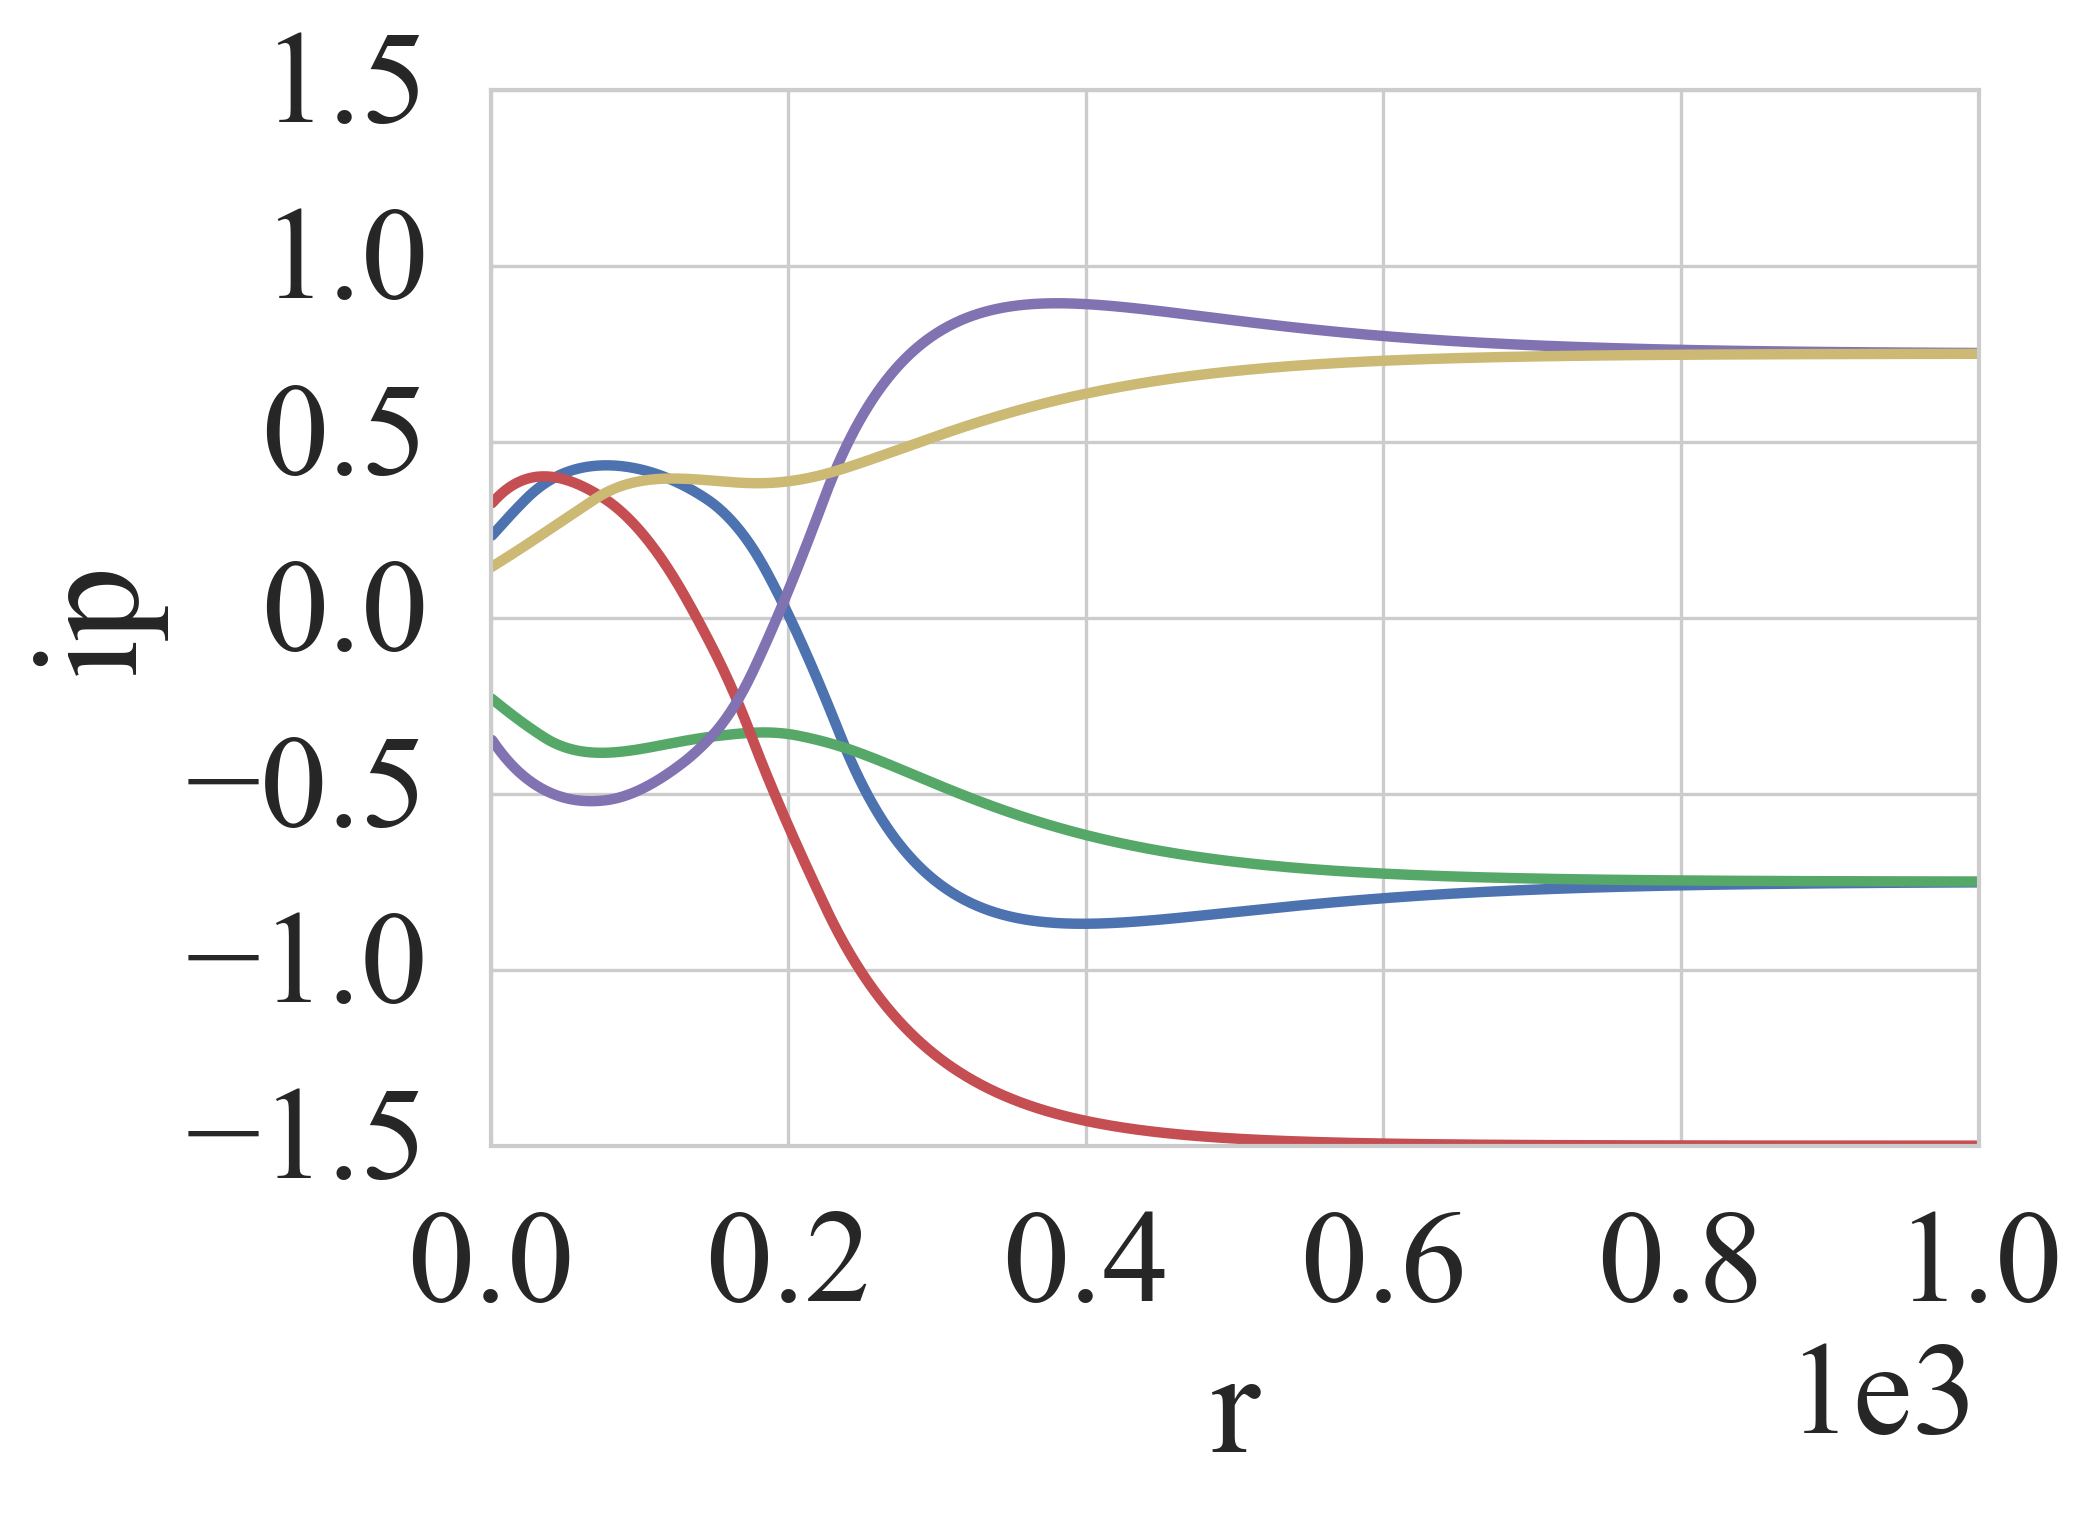
\includegraphics[width=0.4\linewidth,keepaspectratio]{./simulation/diamond/diamond_ip_symmetric_negative.png}\label{fig:diamond_ip_symmetric_negative}}\qquad
			\subfloat[][]{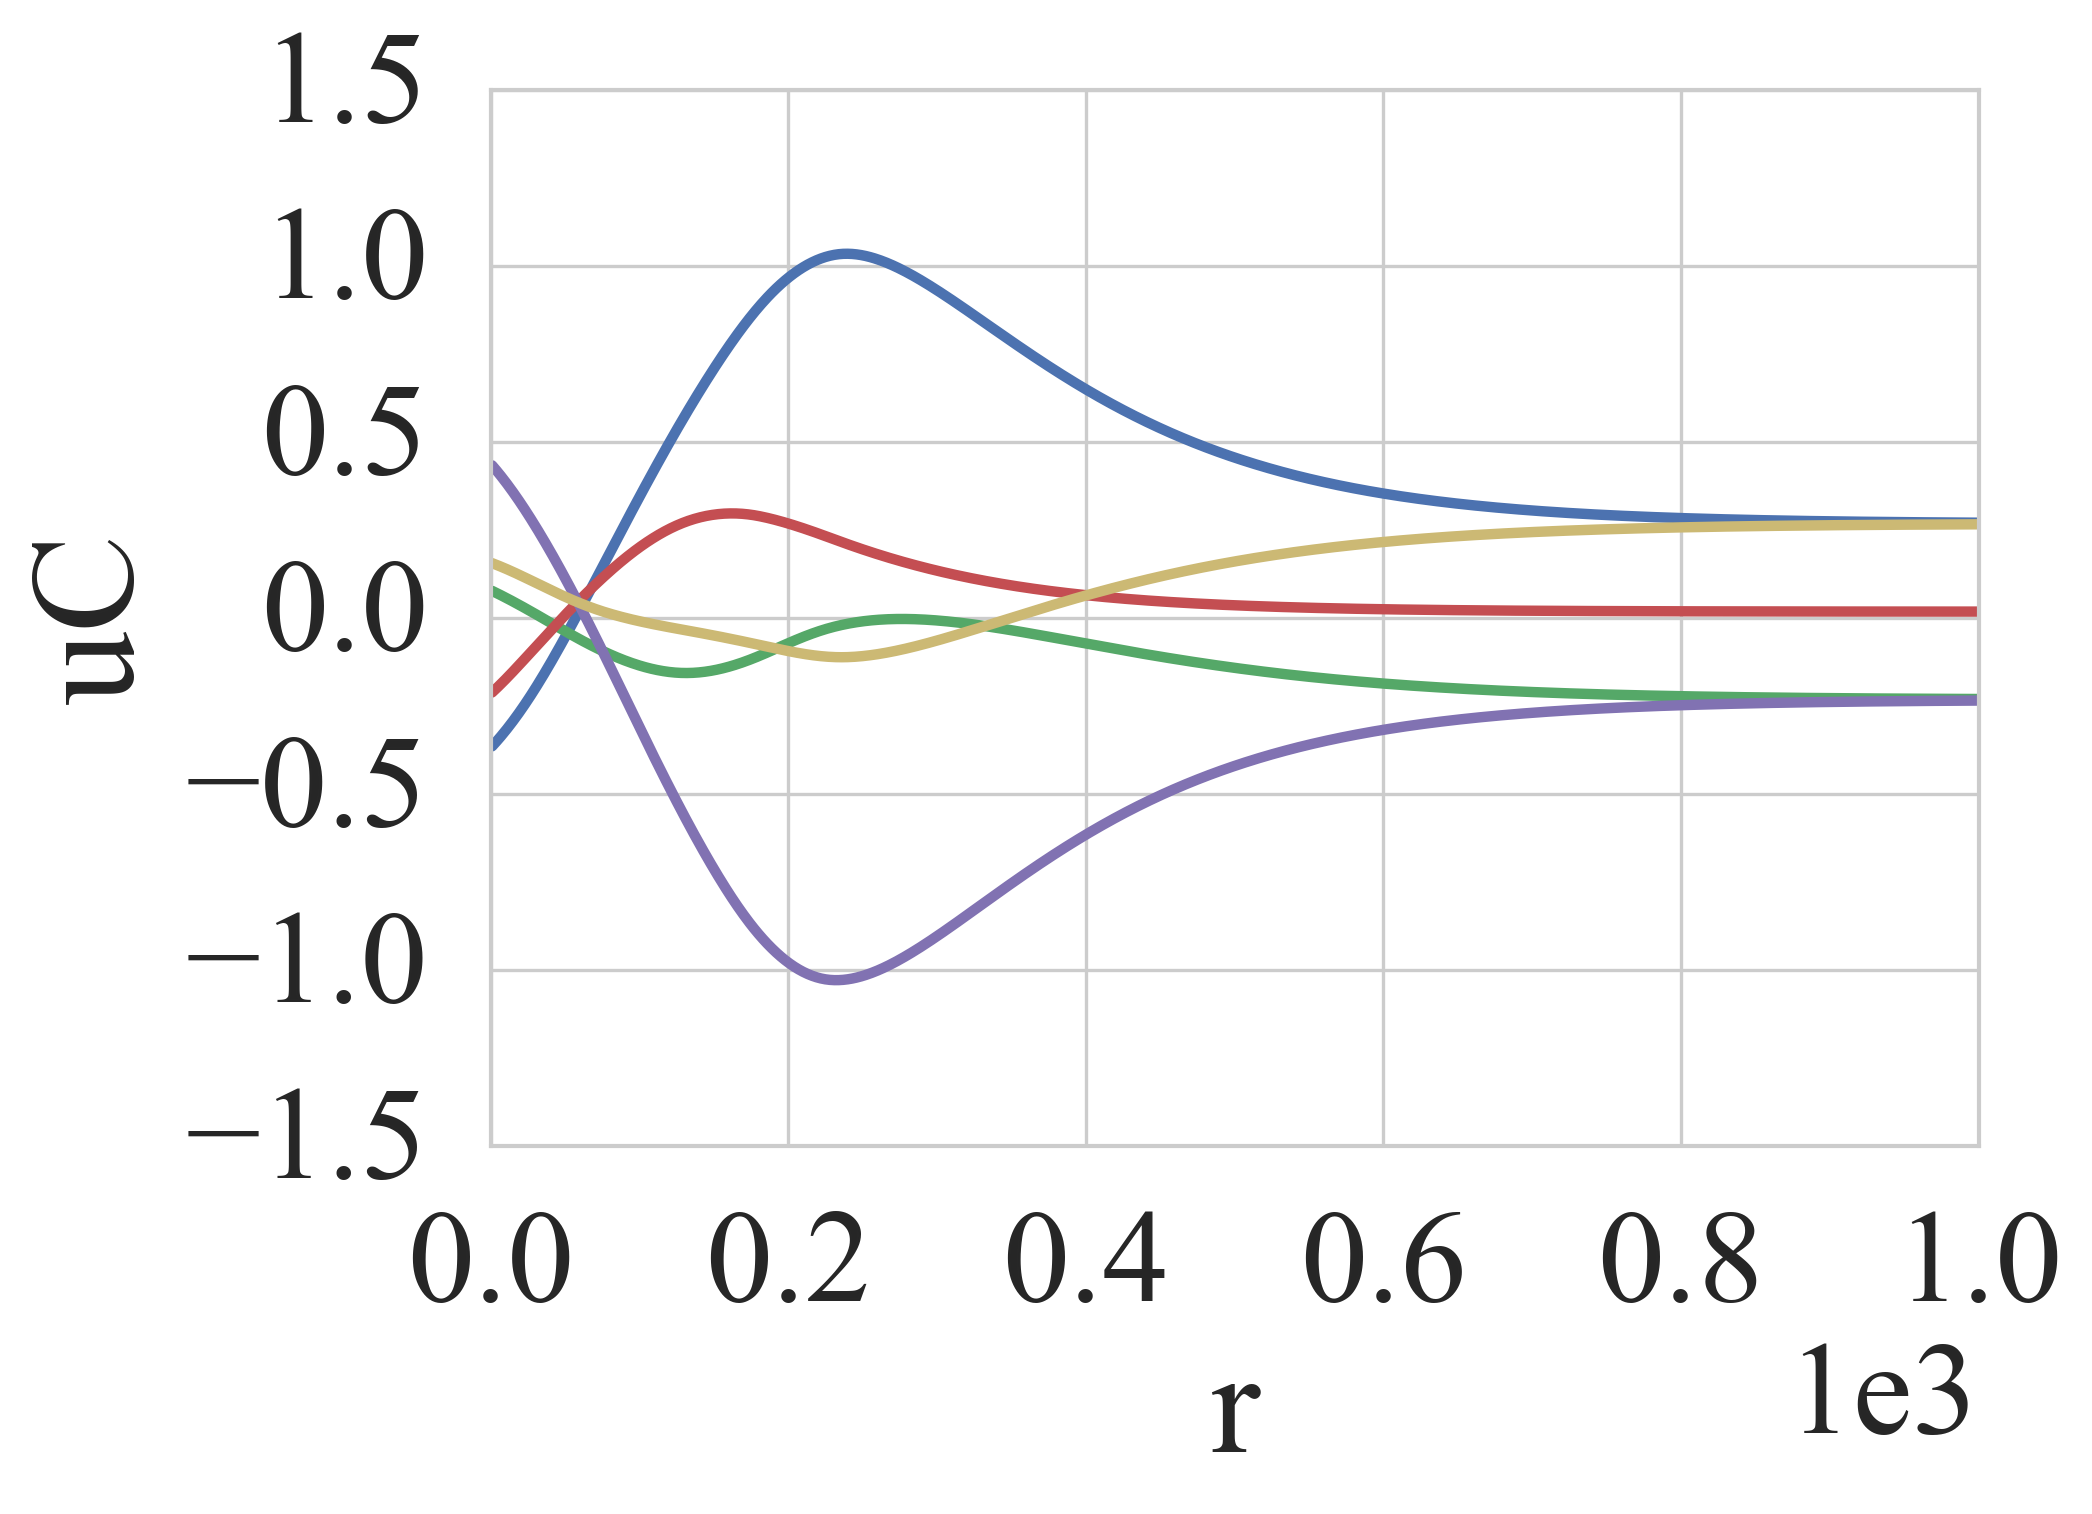
\includegraphics[width=0.4\linewidth,keepaspectratio]{./simulation/diamond/diamond_uC_symmetric_negative.png}\label{fig:diamond_uC_symmetric_negative}}
			\newline
			\subfloat[][]{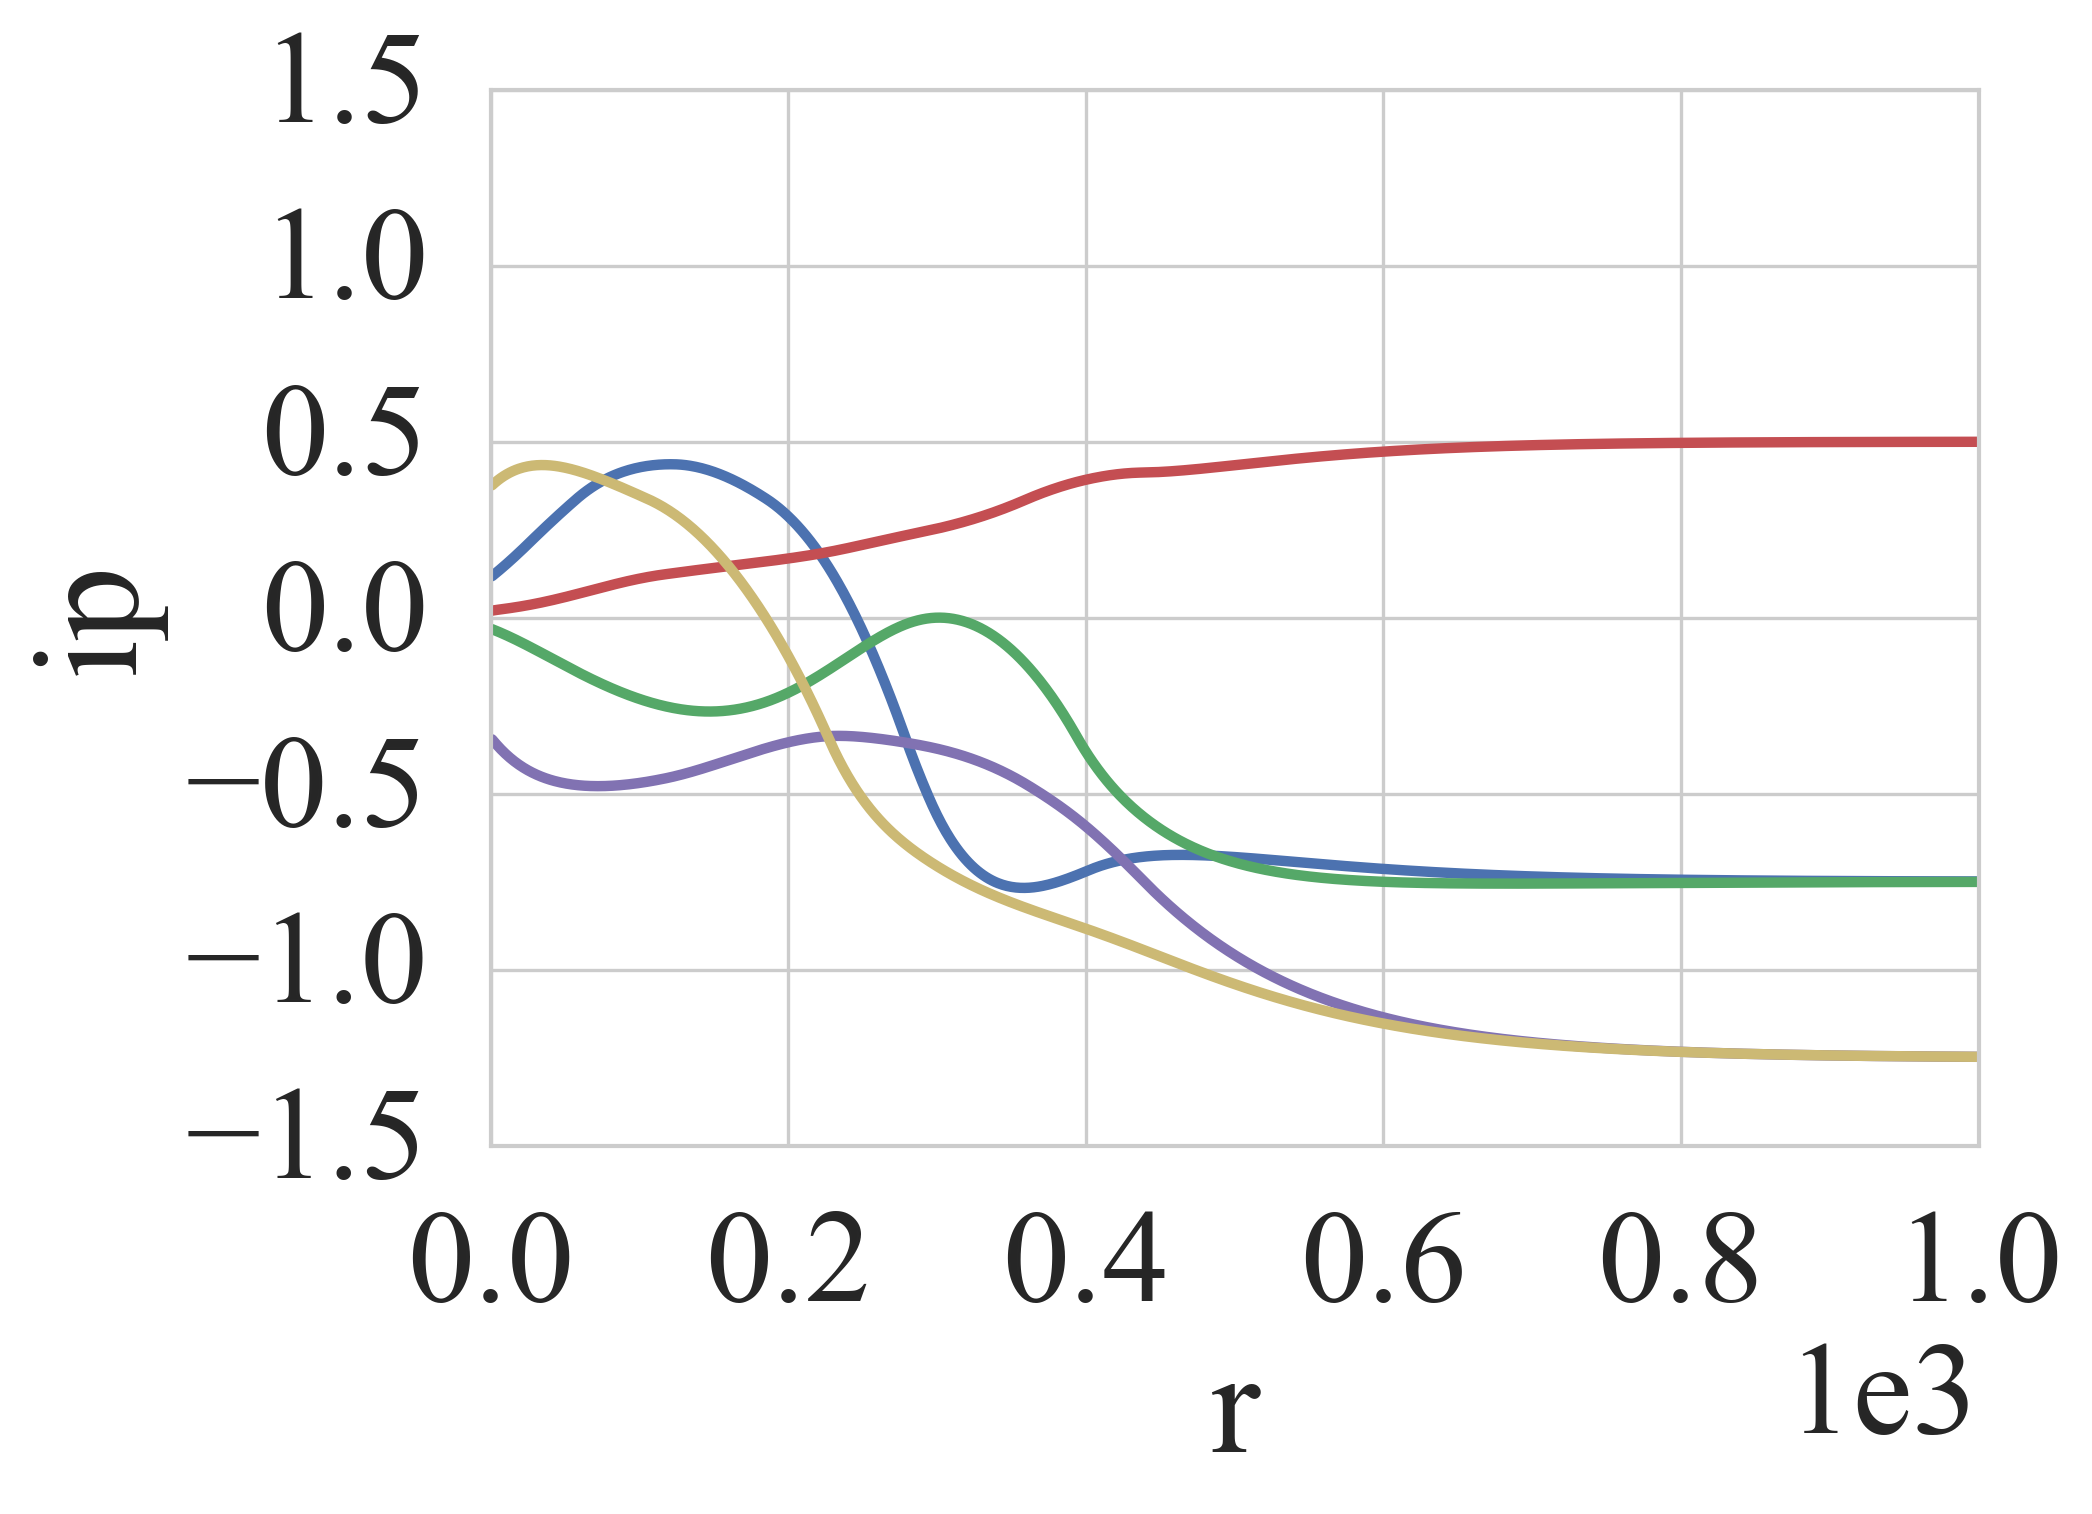
\includegraphics[width=0.4\linewidth,keepaspectratio]{./simulation/diamond/diamond_ip_asymmetric_positive.png}\label{fig:diamond_ip_asymmetric_positive}}\qquad
			\subfloat[][]{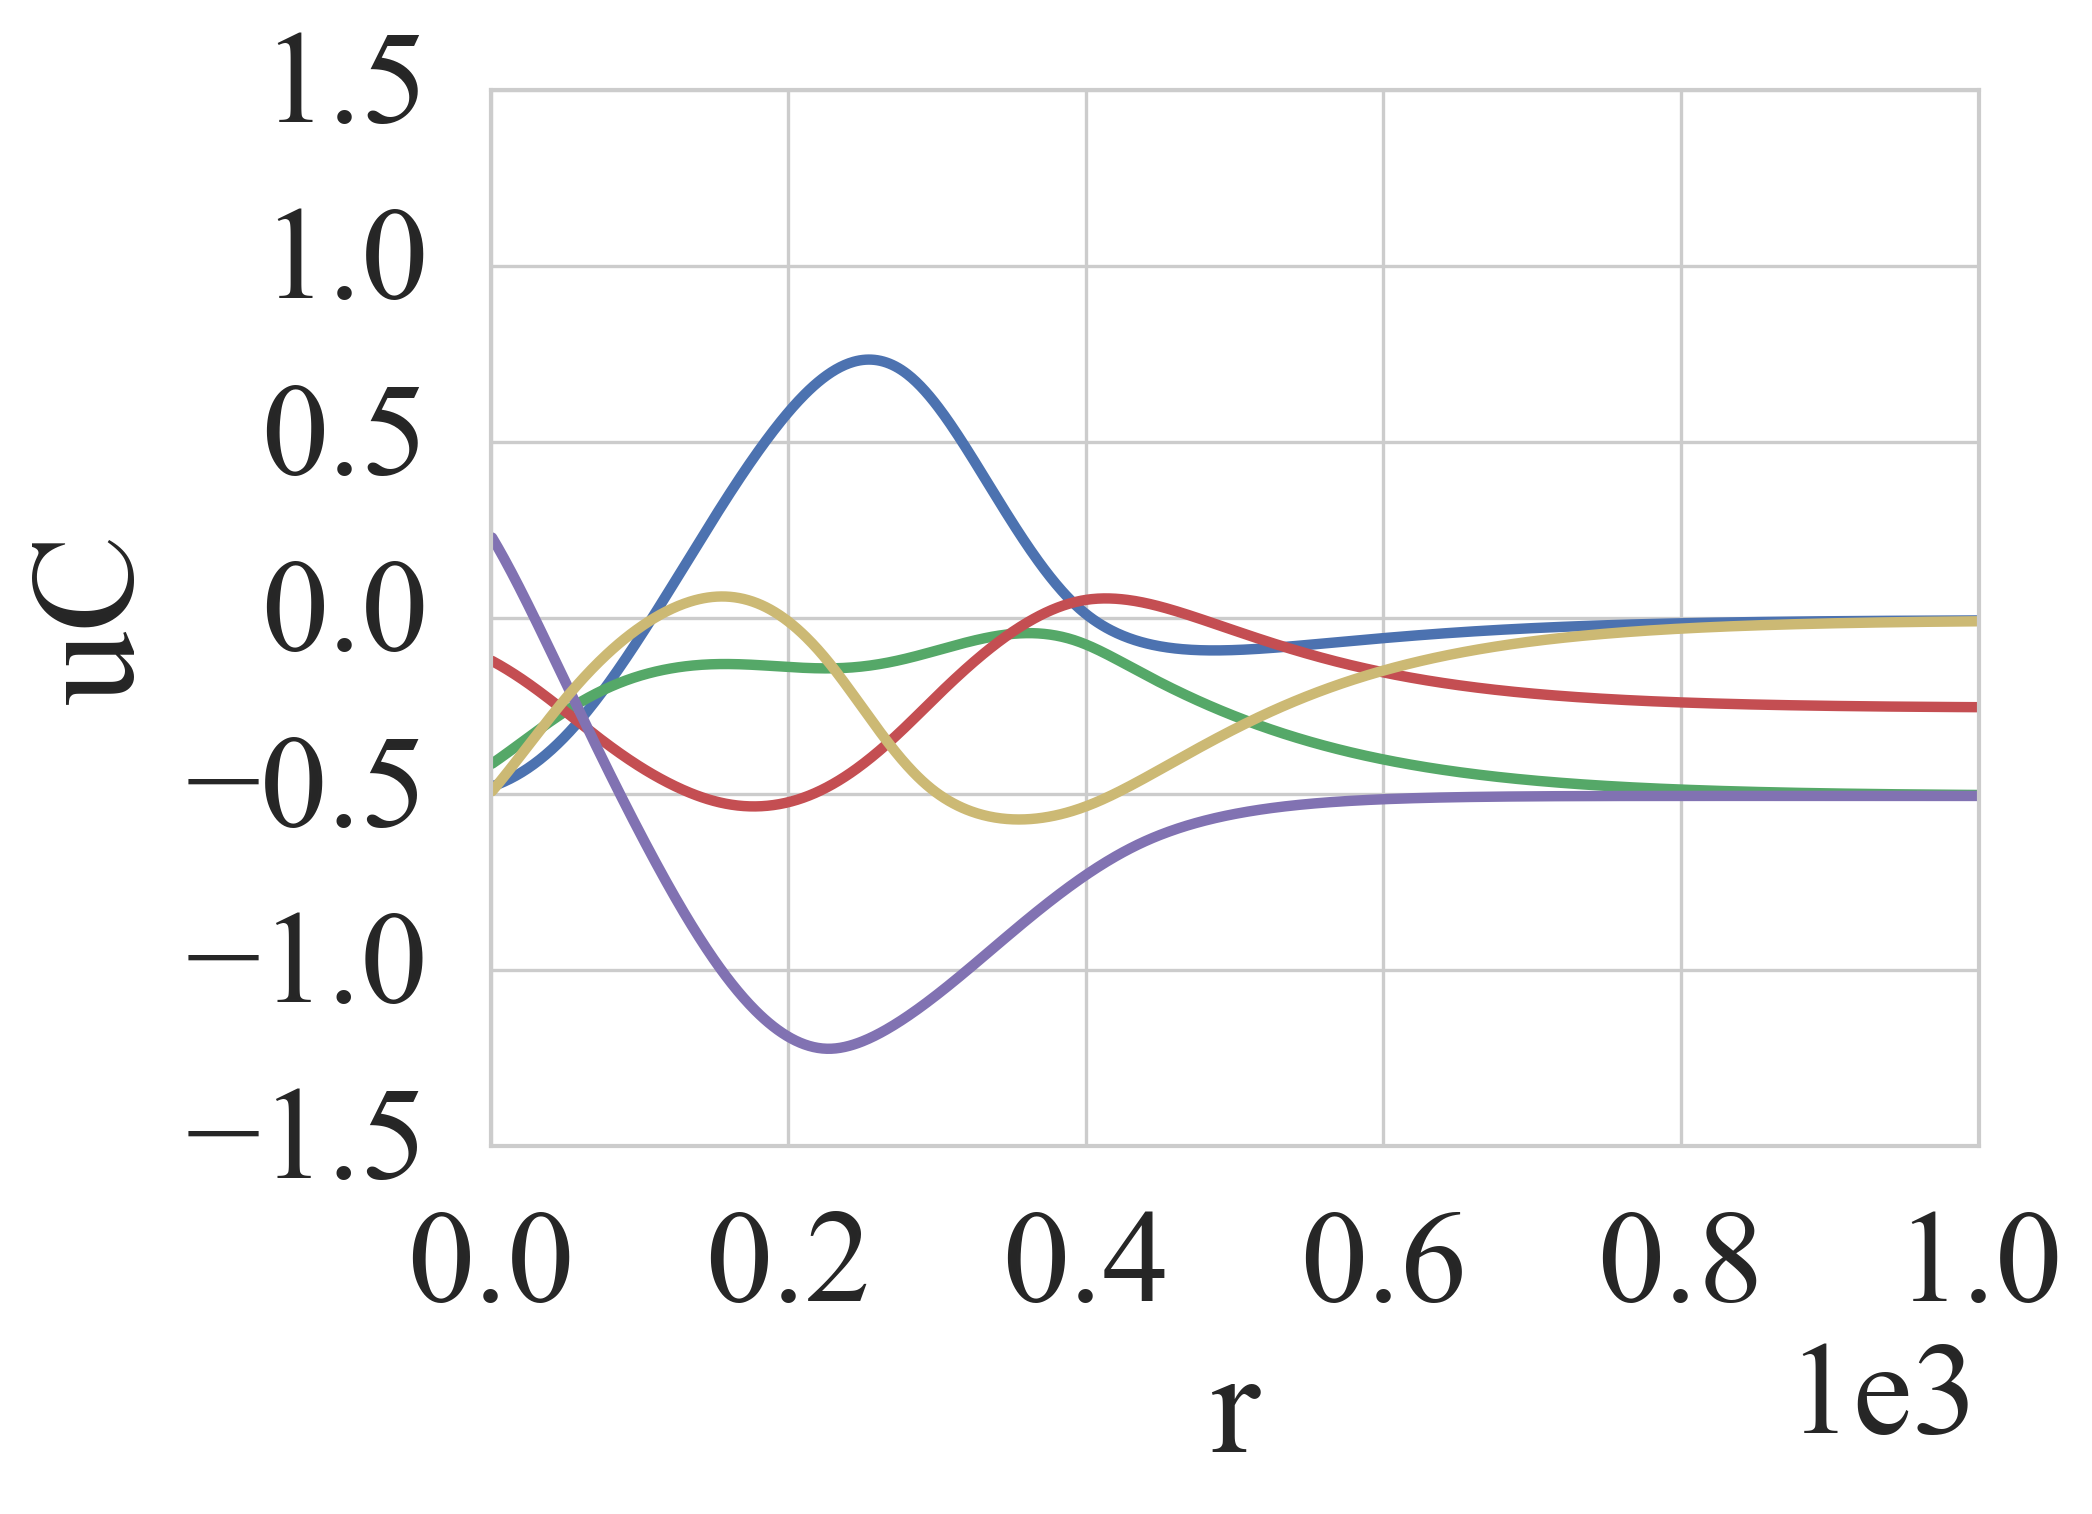
\includegraphics[width=0.4\linewidth,keepaspectratio]{./simulation/diamond/diamond_uC_asymmetric_positive.png}\label{fig:diamond_uC_asymmetric_positive}}
			
			\caption[Simulation - Diamond or Wheatstone graph]{Diamond of \Pes.}
			\label{fig:diamond}
		\end{figure}

		\FloatBarrier

	\subsection{Paths of Physarum Elements}

		Next we look at paths of \Pes. Here no circulation is possible but neighboring \Pes still interact with each other leading to non-zero currents. \Fref{fig:path_5} depicts a path consisting of $5$ chained \Pes. Again \Fref{fig:path_5_legend} defines a color coding which serves as a legend for the remaining plots of \Fref{fig:paths}. We show the results of three different sub-path of \Fref{fig:path_5} all starting at node $0$. The paths have lengths $l \in [2,3,4]$.

		First, note the capacitor voltages of at least one edge does not converge for any of the depicted paths, see \Fref{fig:path_3_uC}, \Fref{fig:path_4_uC} and \Fref{fig:path_5_uC}. Almost all voltages are quasi-periodic and thus none of these \Pes is converged. 

		A similar behavior is observed for the currents illustrated in \Fref{fig:path_3_ip}, \Fref{fig:path_4_ip} as well as \Fref{fig:path_5_ip}. Note that for all paths we find that the currents of all but one edge periodically reverse their signs, \ie flow reversal occurs naturally. At present, we do not know why there remains one edge with zero flow.

		The distinguishing feature of these \Pes seems to be the period of the oscillations. For paths of length $3$ we repeated the simulation $100$ times with different random initial conditions. Without fail the \Pn produced a signal with a period of $T = 1087$ rounds in every execution. We thus conclude that the period is invariant under initial conditions within the ranges we explored. 

		Furthermore, we find that the period of the oscillations decreases with increasing path length. For small path lengths the observed values suggest a linear relation between path length and period as a best fit. To explore the matter further we extended the simulations to paths lengths of up to $10$. We found that a simple functional relationship between path length and period cannot be confirmed for all tested lengths. Rather, for path lengths longer than $7$ more complicated oscillation patters are found to repeat themselves. Here it appears that higher order oscillations come into play. At present their meaning is not clear to the authors. We conclude, however, that there is complex relation between the oscillation patterns and the size of the underlying \Pes that warrants further exploration.

		Another aspect awaiting investigation is the nature of the phase shifts observed between the edges of the circuits. 
                
		\begin{figure}
			\centering
			\subfloat[][]{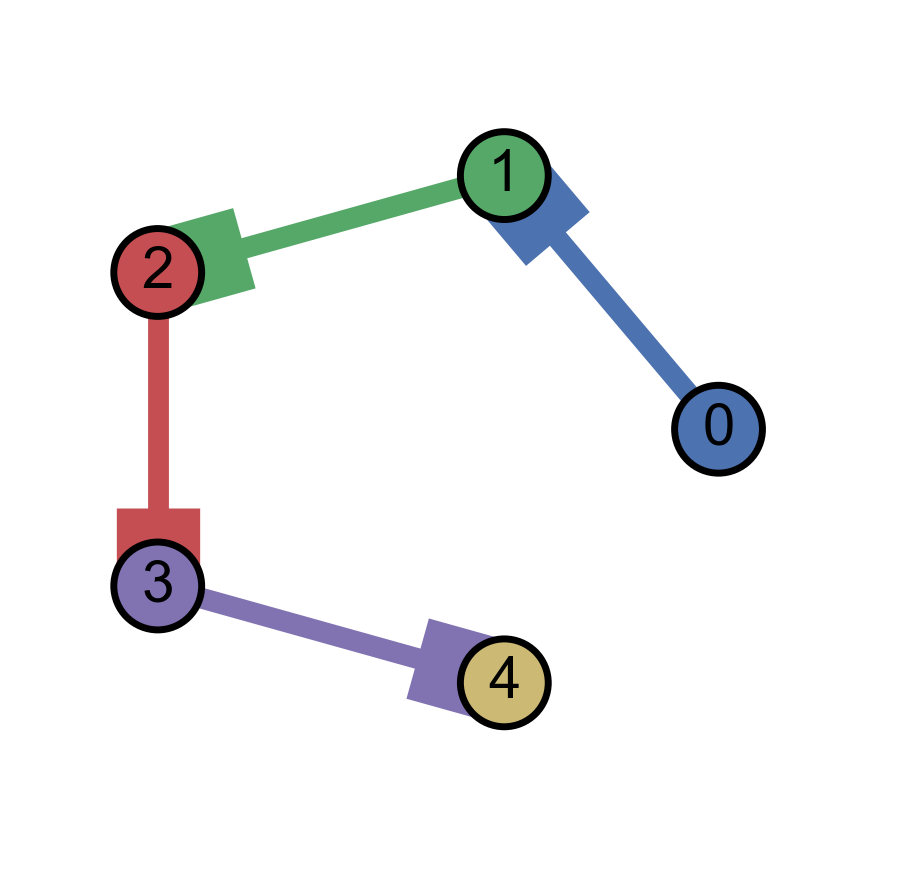
\includegraphics[width=0.4\linewidth,keepaspectratio,trim={0 3cm 0 3cm},clip]{./simulation/path/path_5.png}\label{fig:path_5}}\qquad
			\subfloat[][]{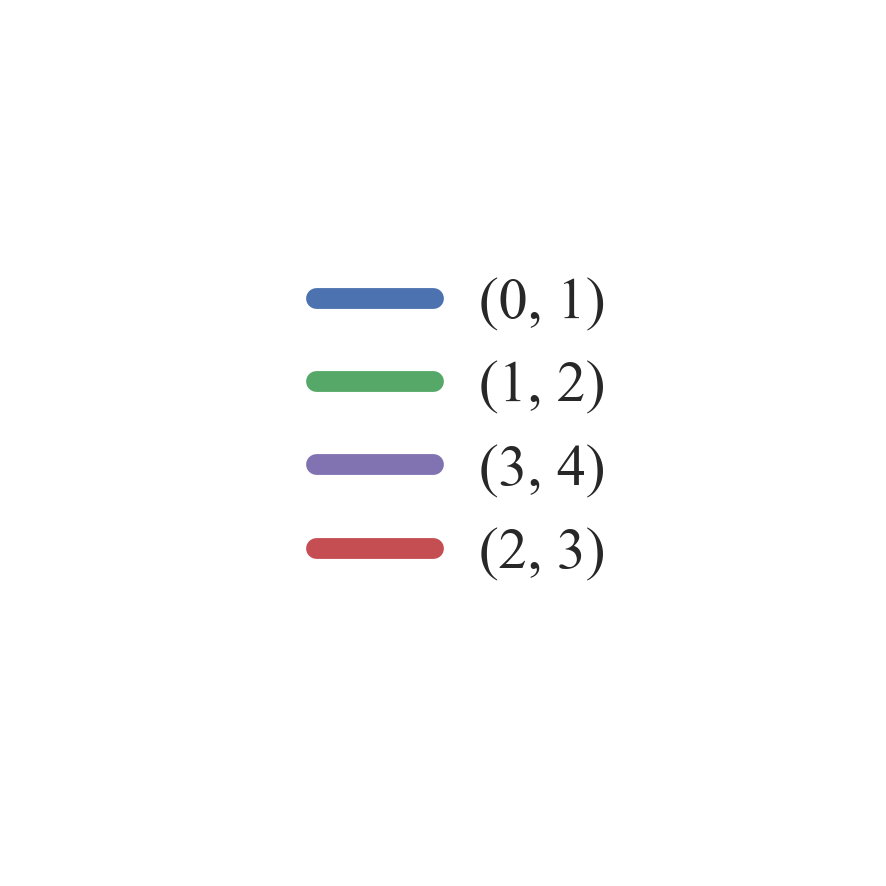
\includegraphics[width=0.4\linewidth,keepaspectratio,trim={0 3cm 0 3cm},clip]{./simulation/path/path_5_legend.png}\label{fig:path_5_legend}}
			\newline
			\subfloat[][Period $T \approx 694$ rounds.]{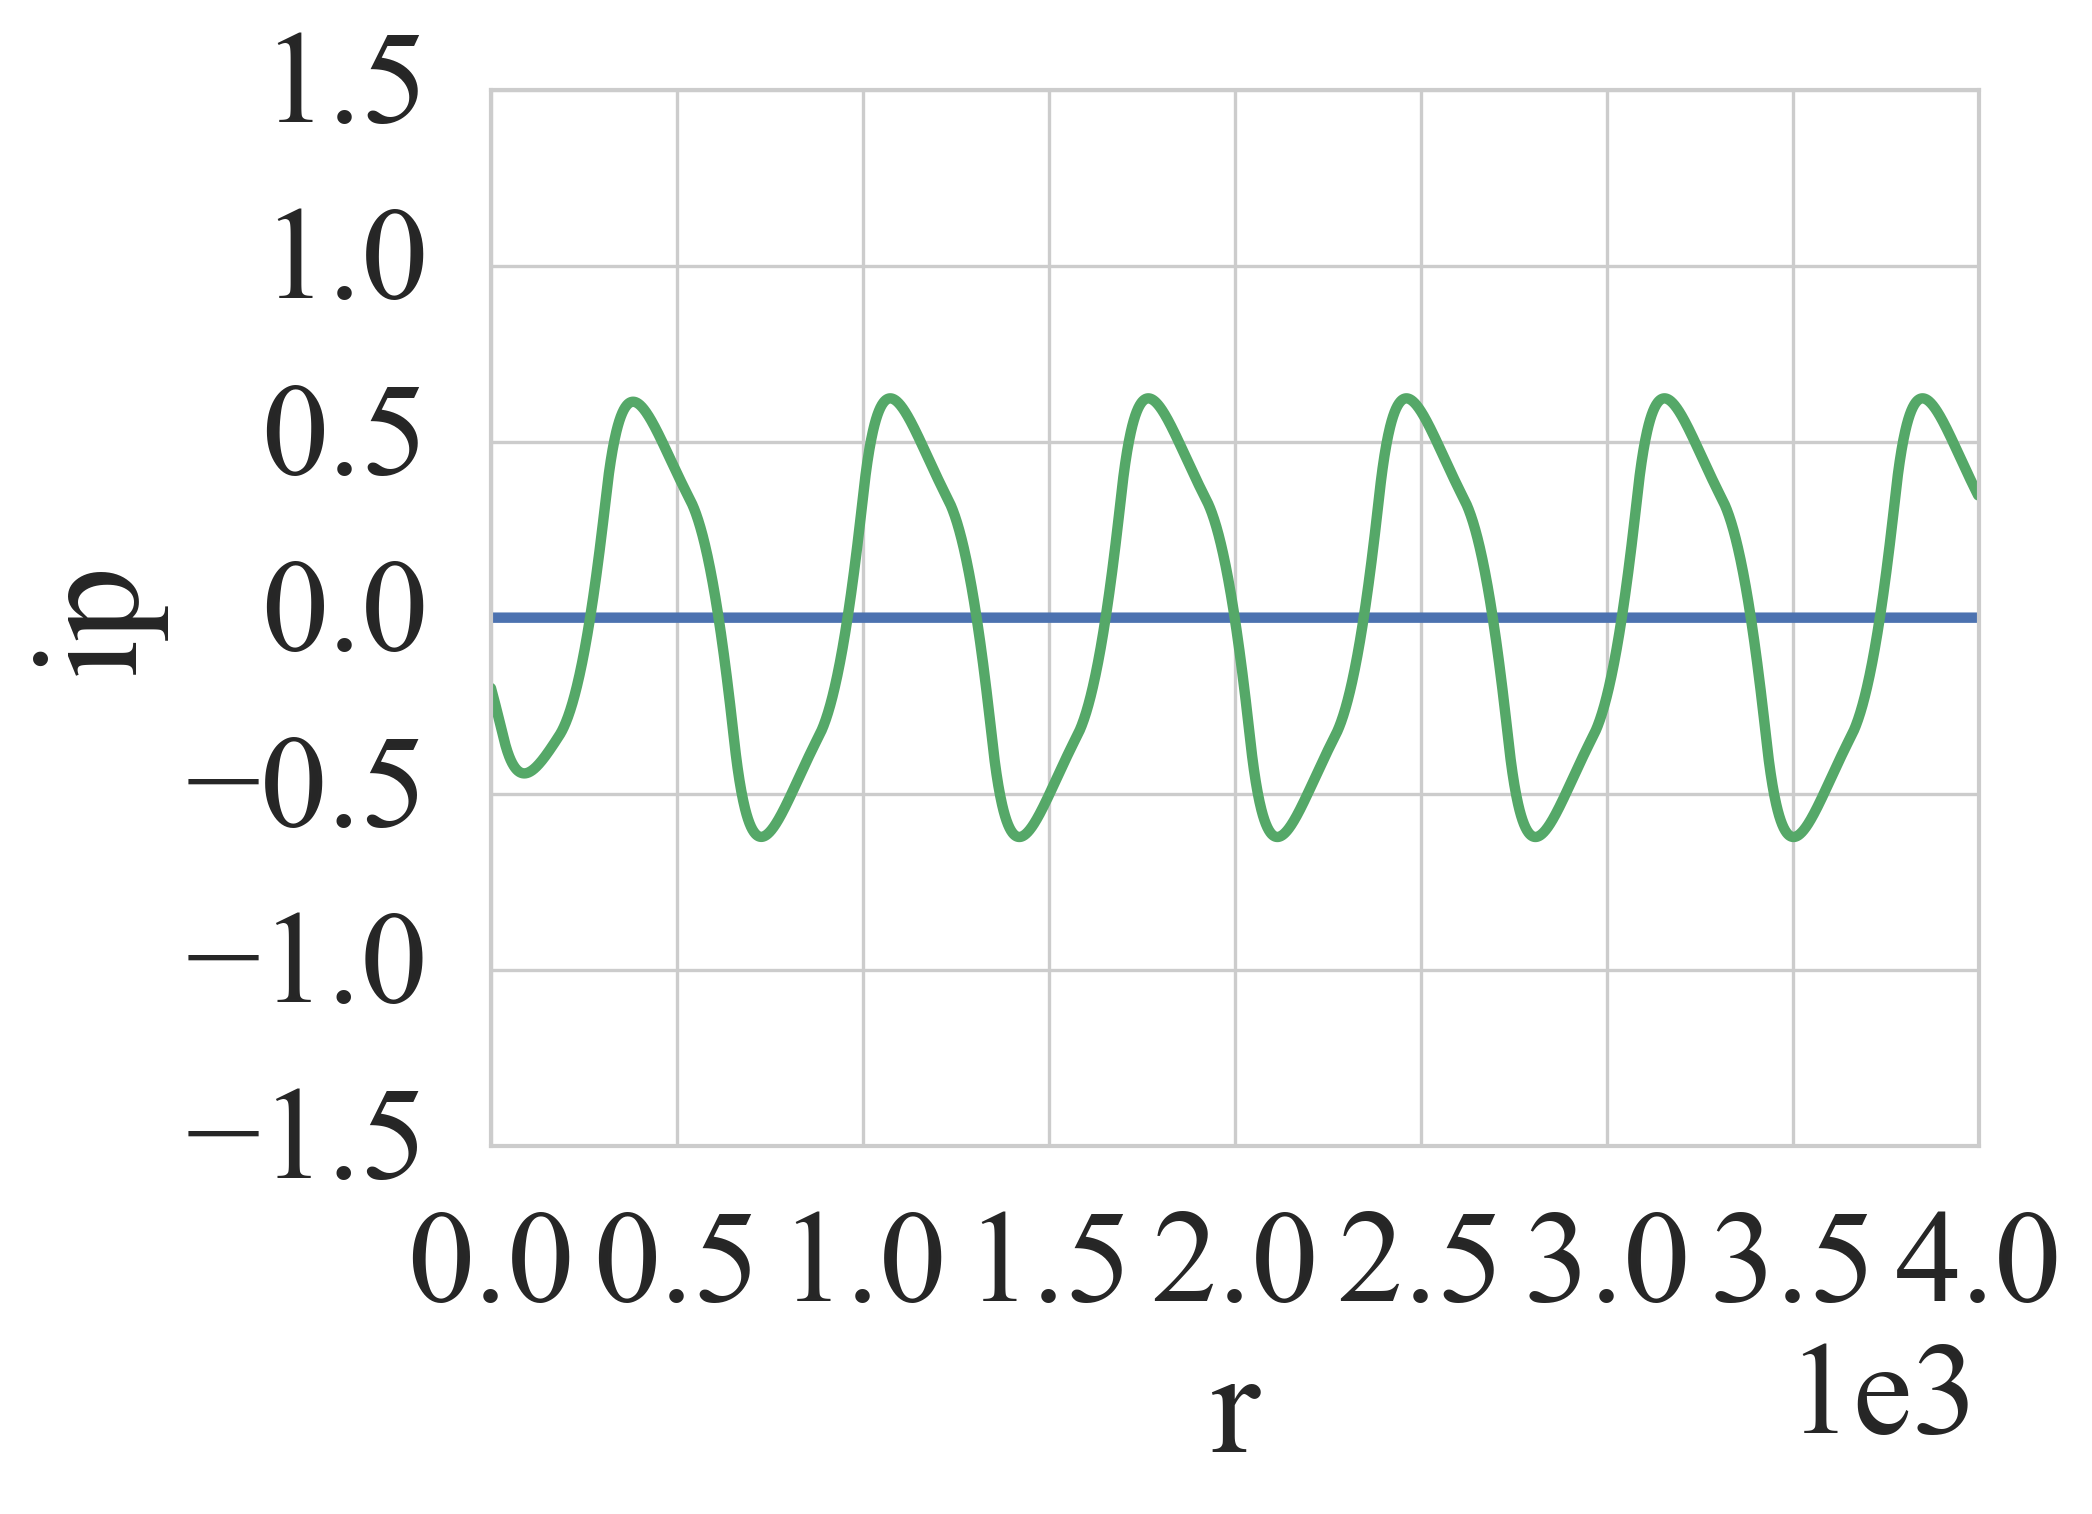
\includegraphics[width=0.4\linewidth,keepaspectratio]{./simulation/path/path_3_ip.png}\label{fig:path_3_ip}}\qquad
			\subfloat[][Period $T \approx 694$ rounds.]{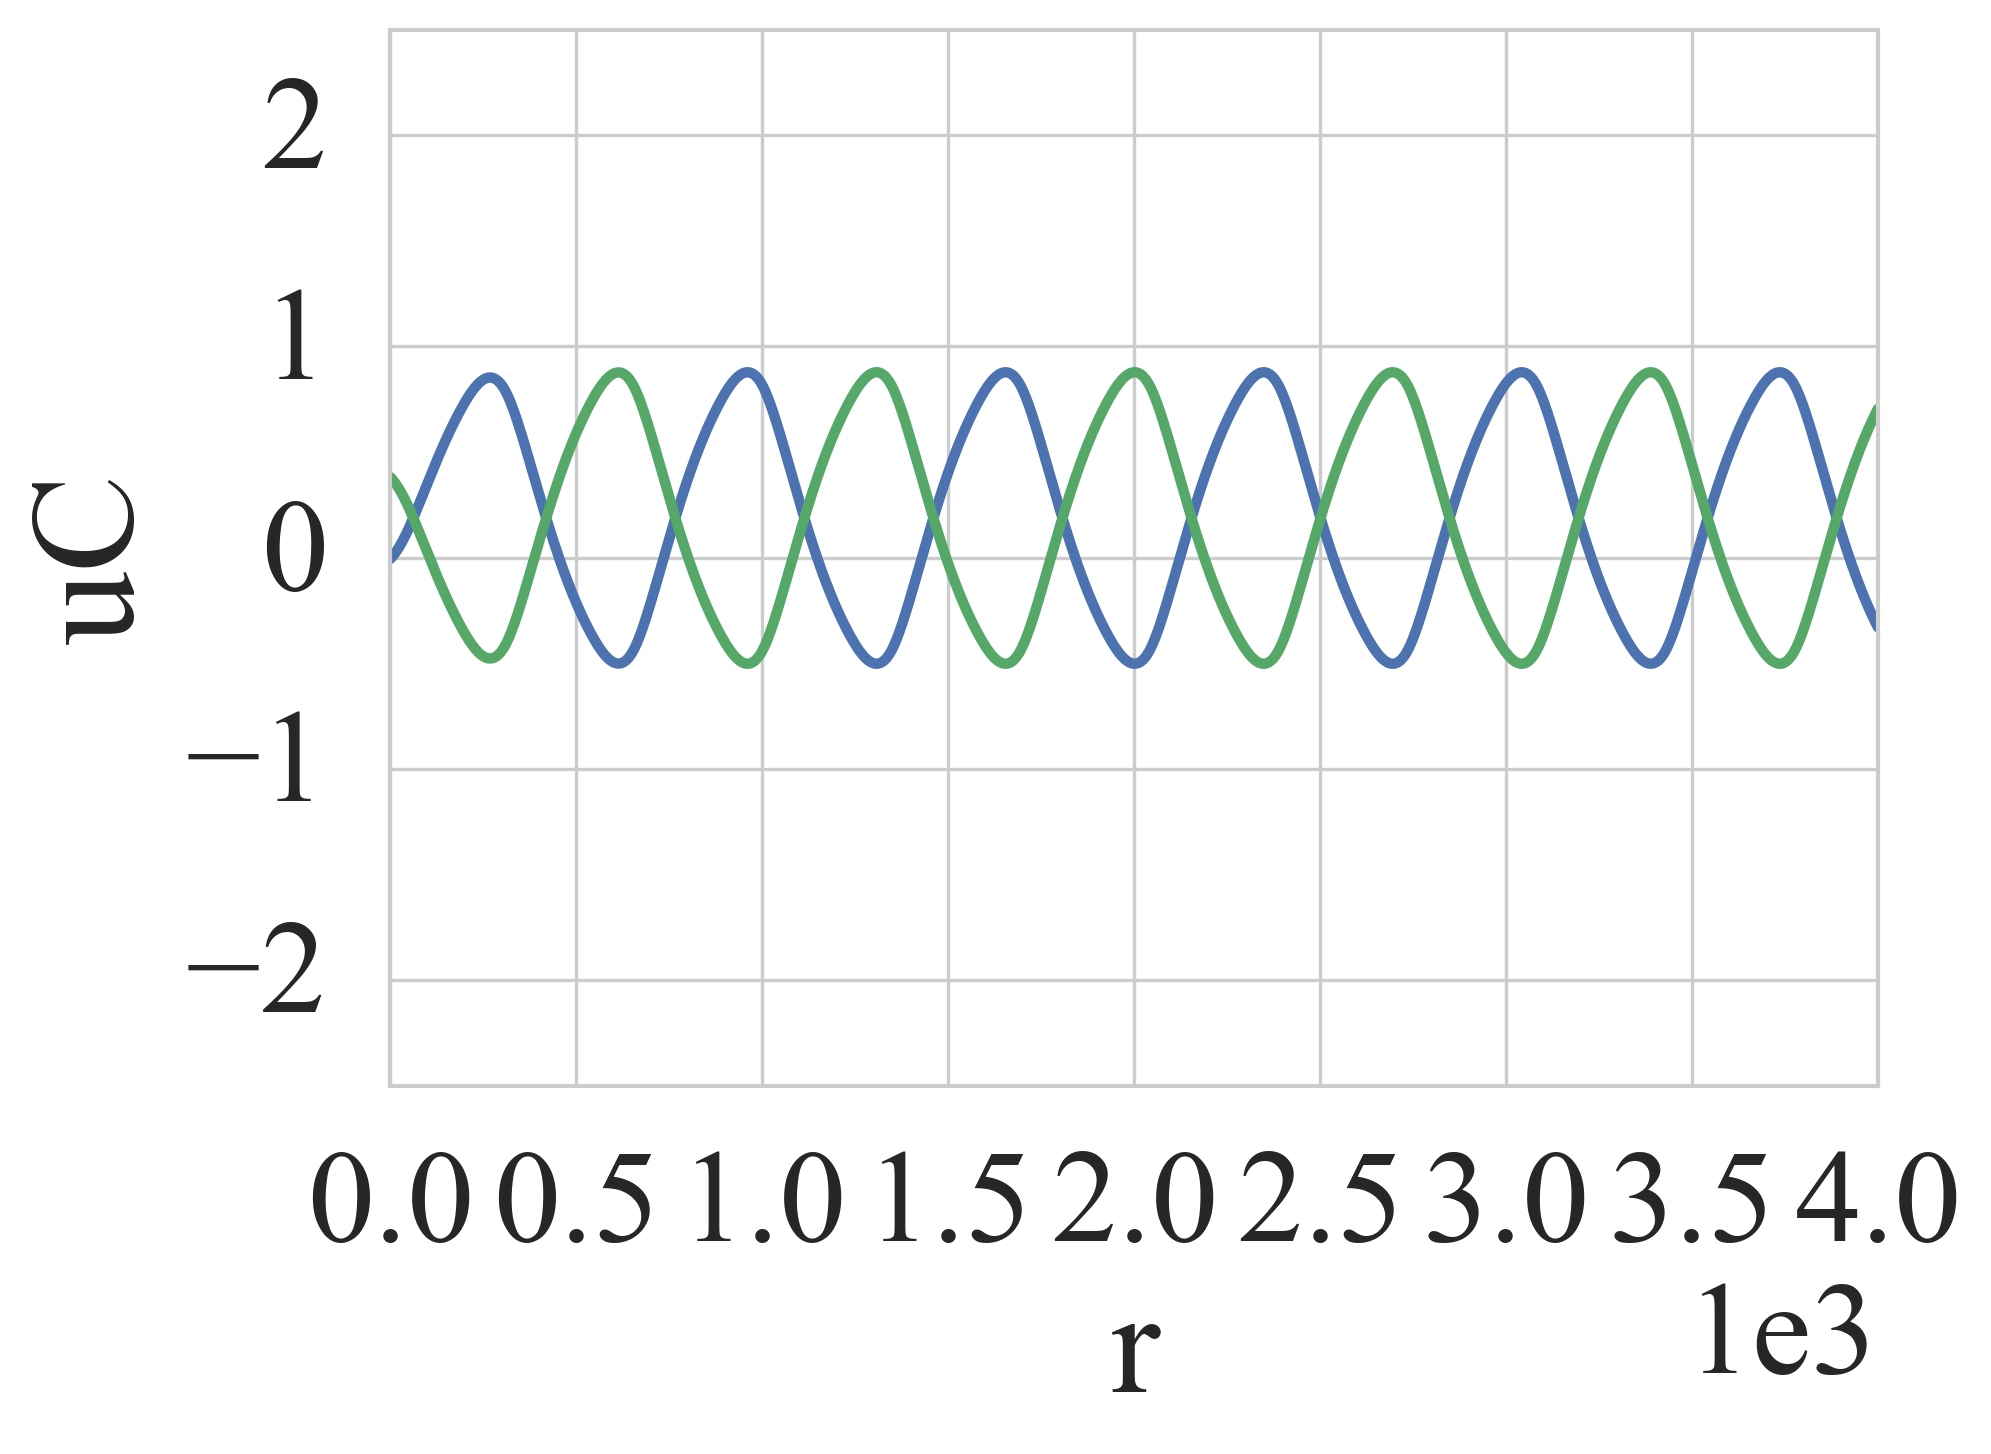
\includegraphics[width=0.4\linewidth,keepaspectratio]{./simulation/path/path_3_uC.png}\label{fig:path_3_uC}}
			\newline
			\subfloat[][Period $T \approx 1087$ rounds.]{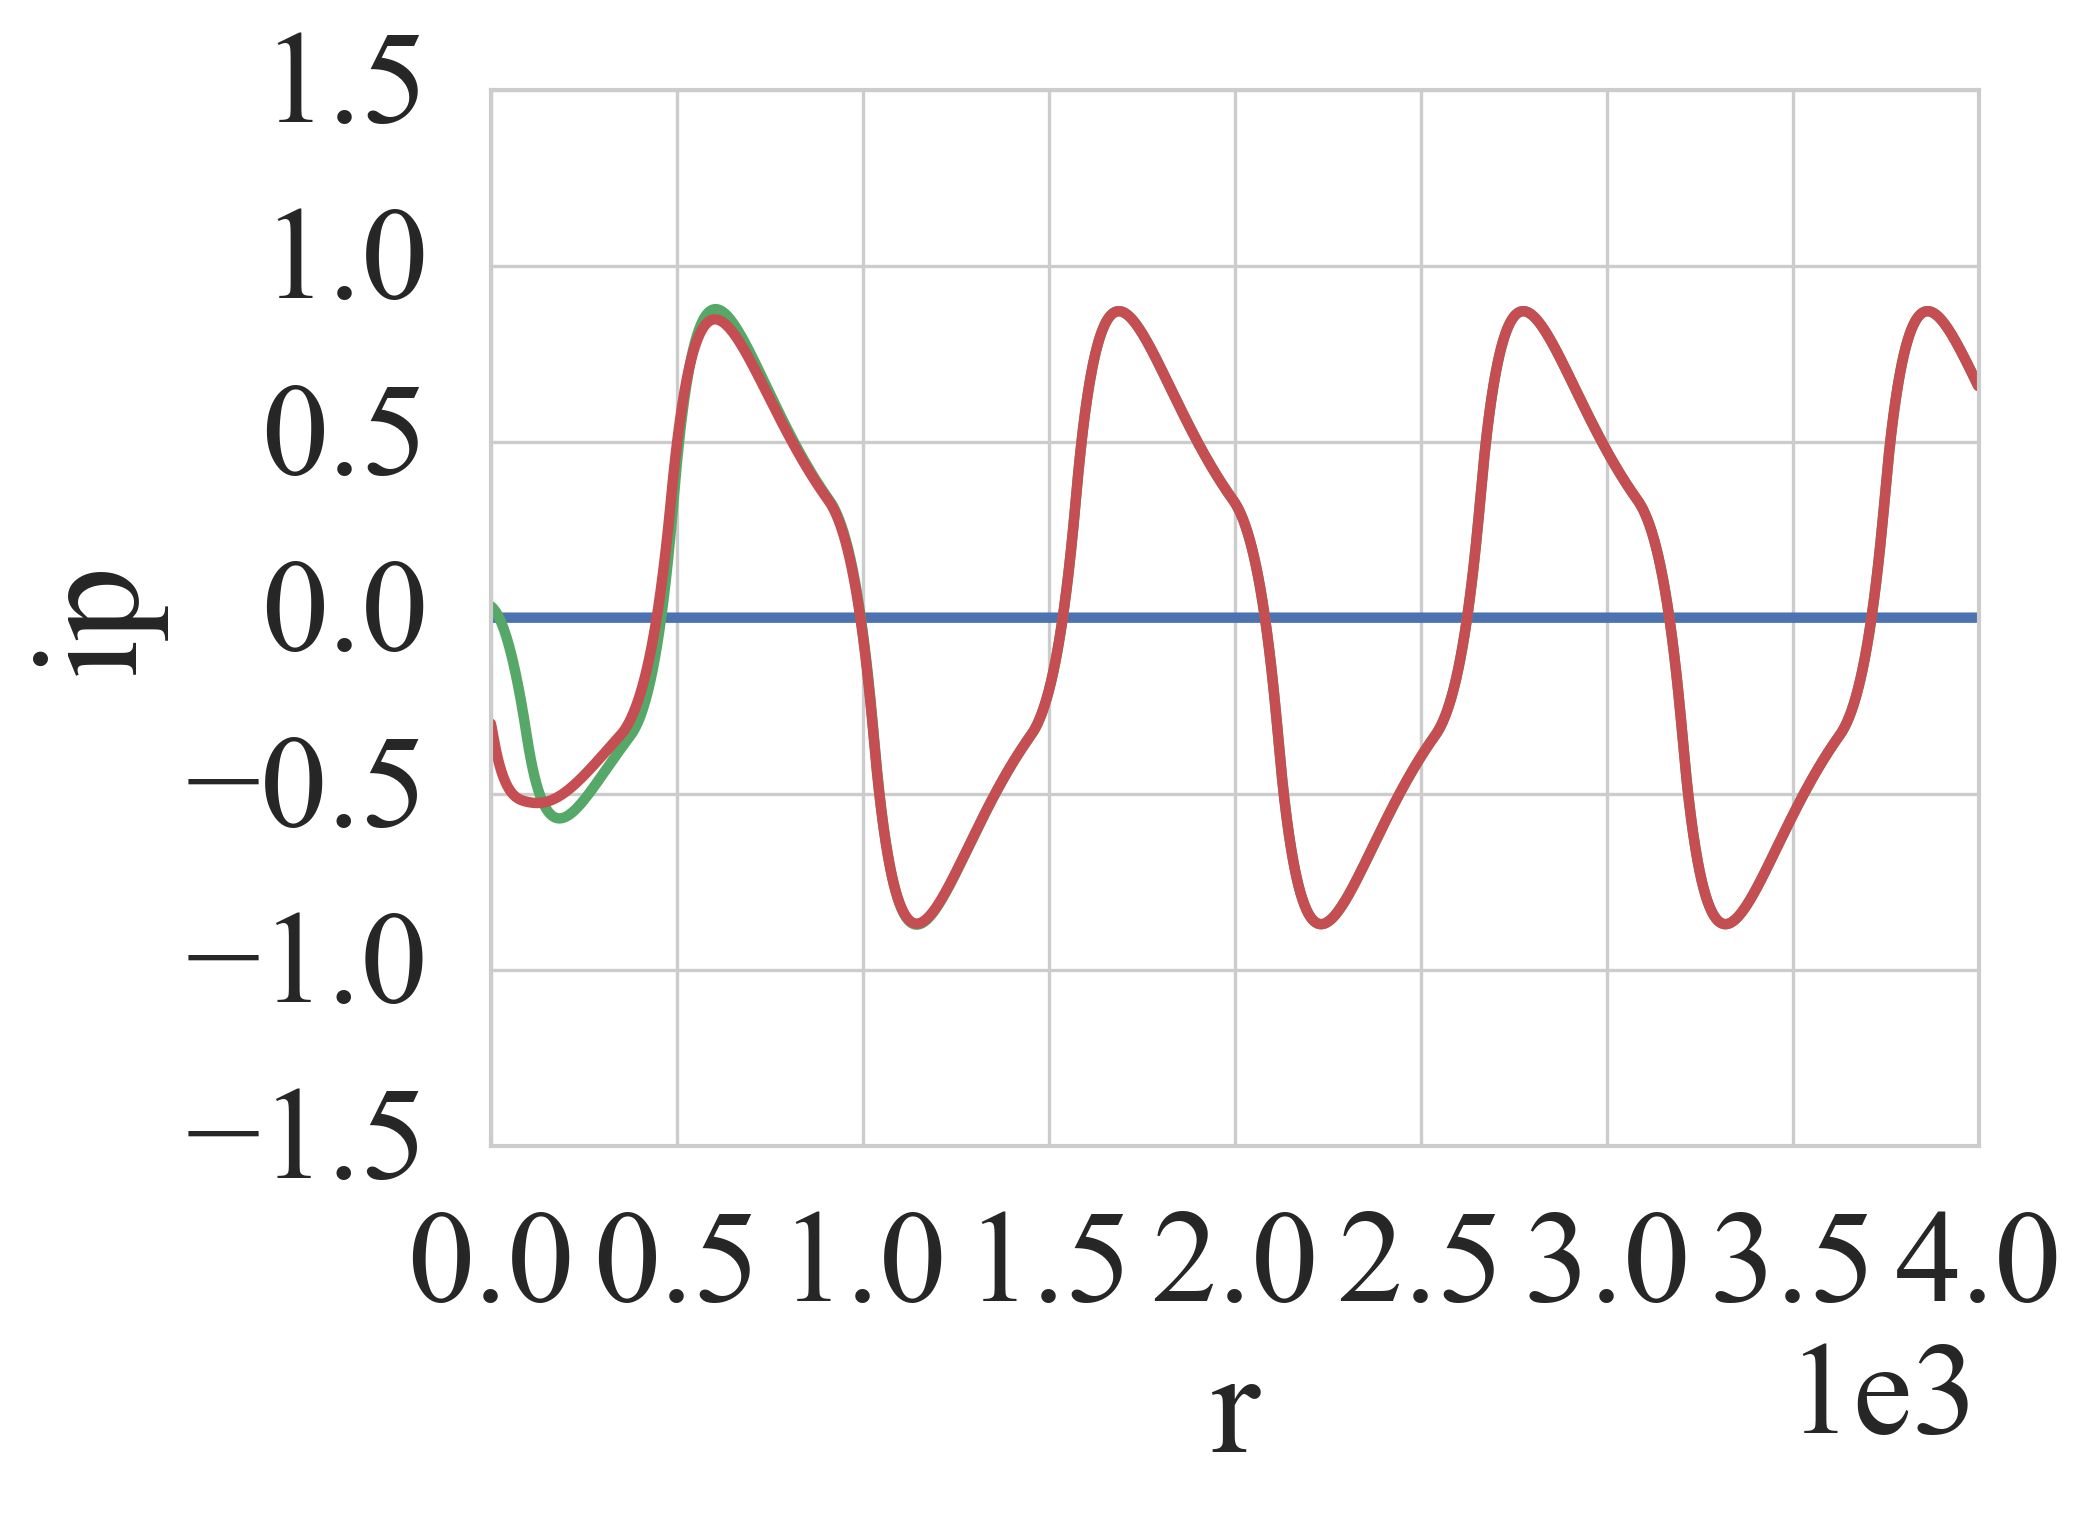
\includegraphics[width=0.4\linewidth,keepaspectratio]{./simulation/path/path_4_ip.png}\label{fig:path_4_ip}}\qquad
			\subfloat[][Period $T \approx 1087$ rounds.]{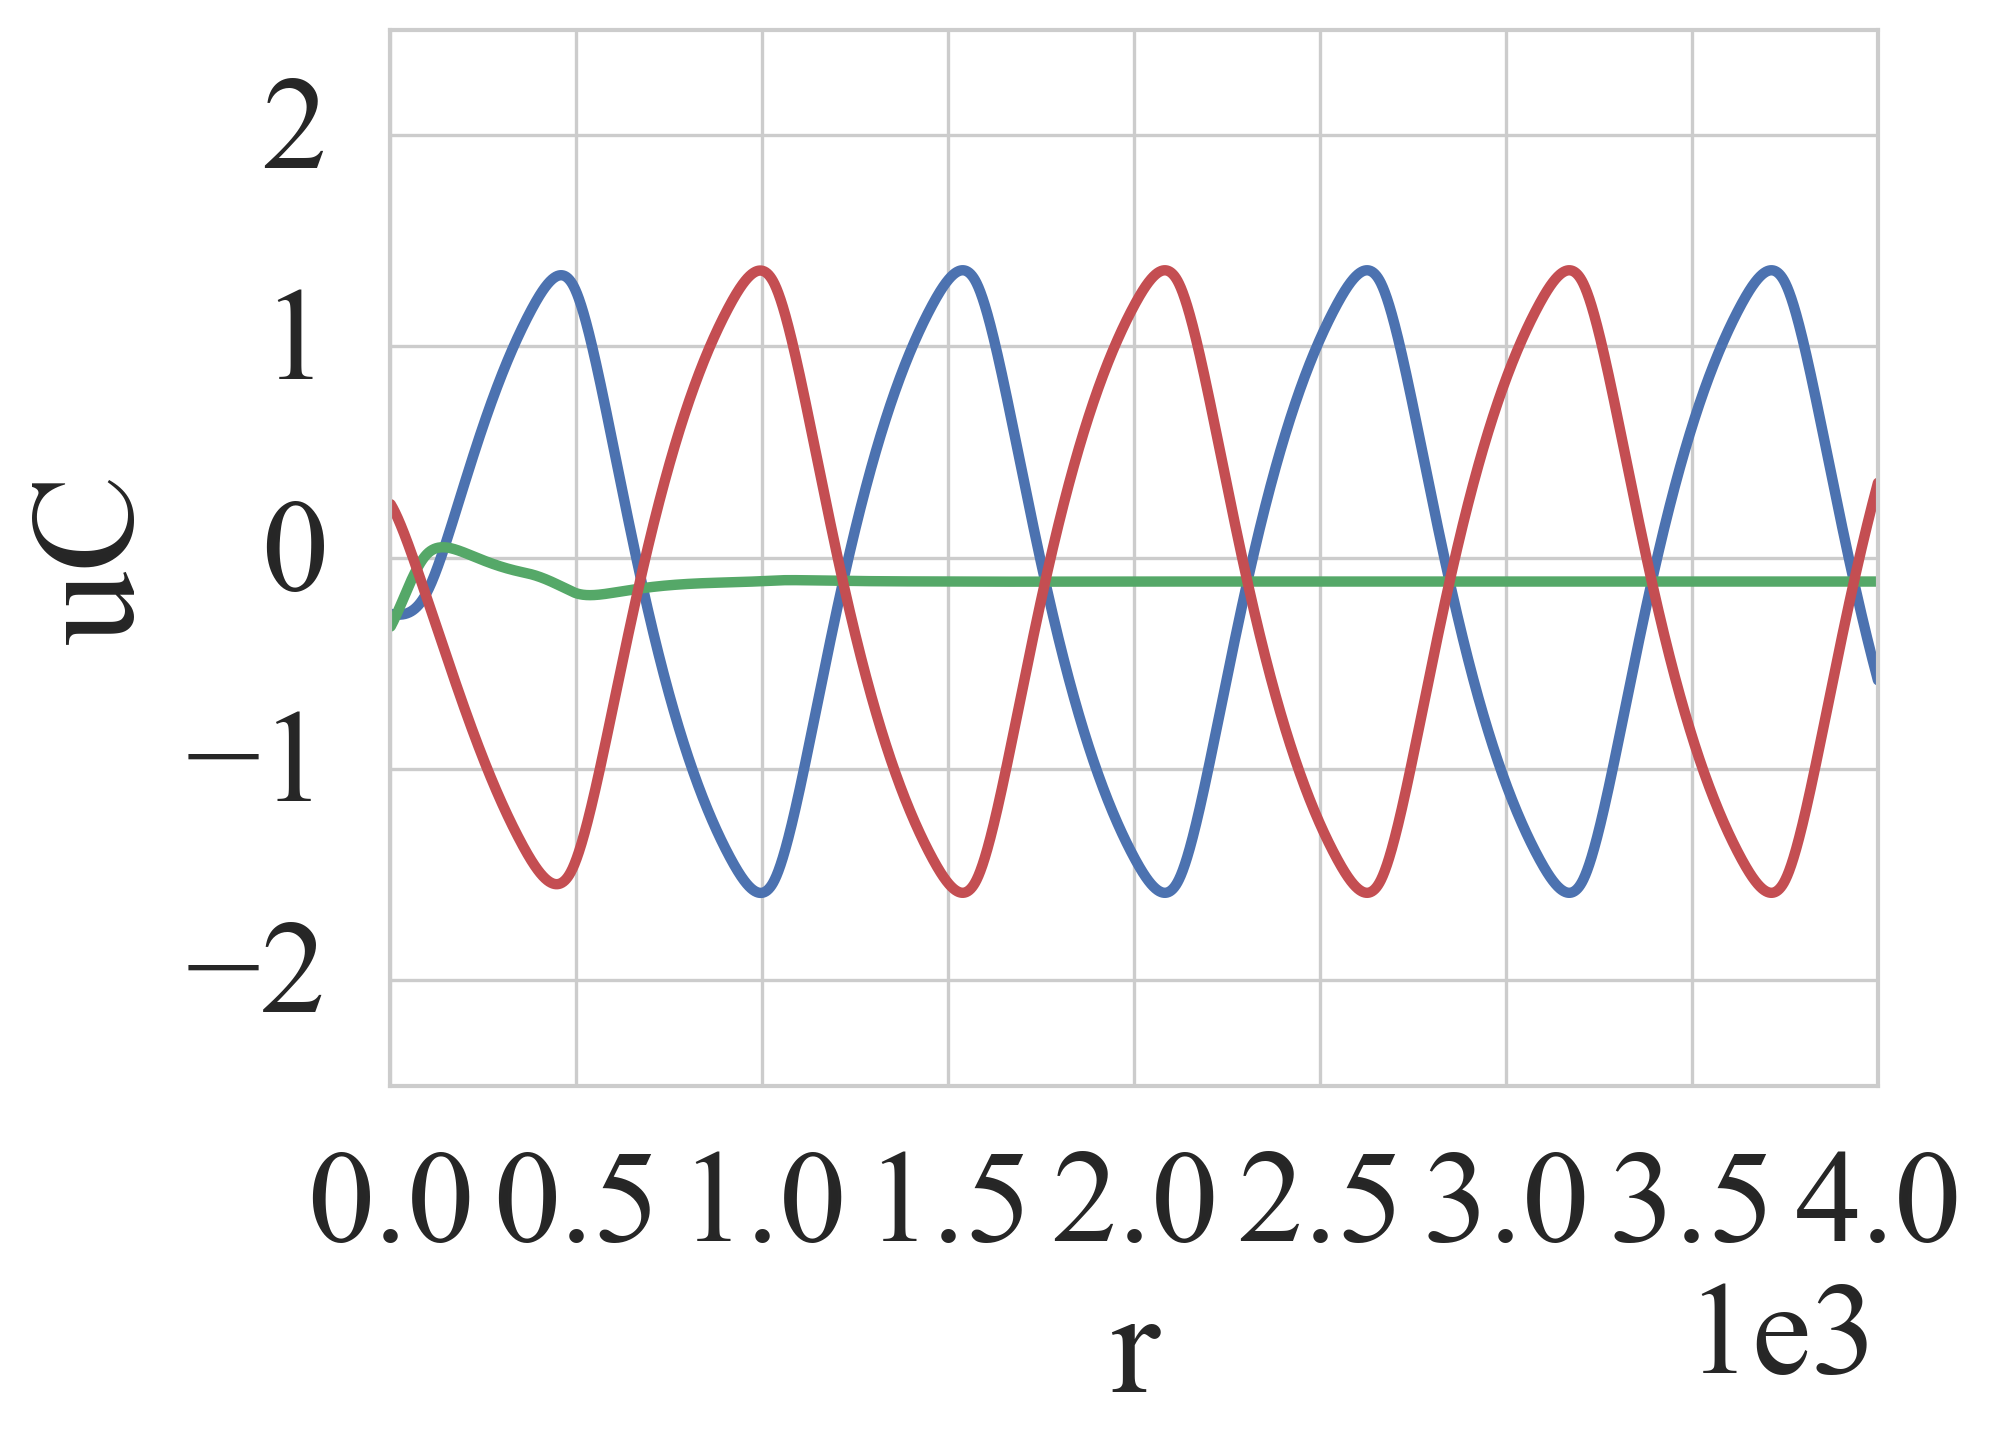
\includegraphics[width=0.4\linewidth,keepaspectratio]{./simulation/path/path_4_uC.png}\label{fig:path_4_uC}}
			\newline
			\subfloat[][Period $T \approx 1522$ rounds.]{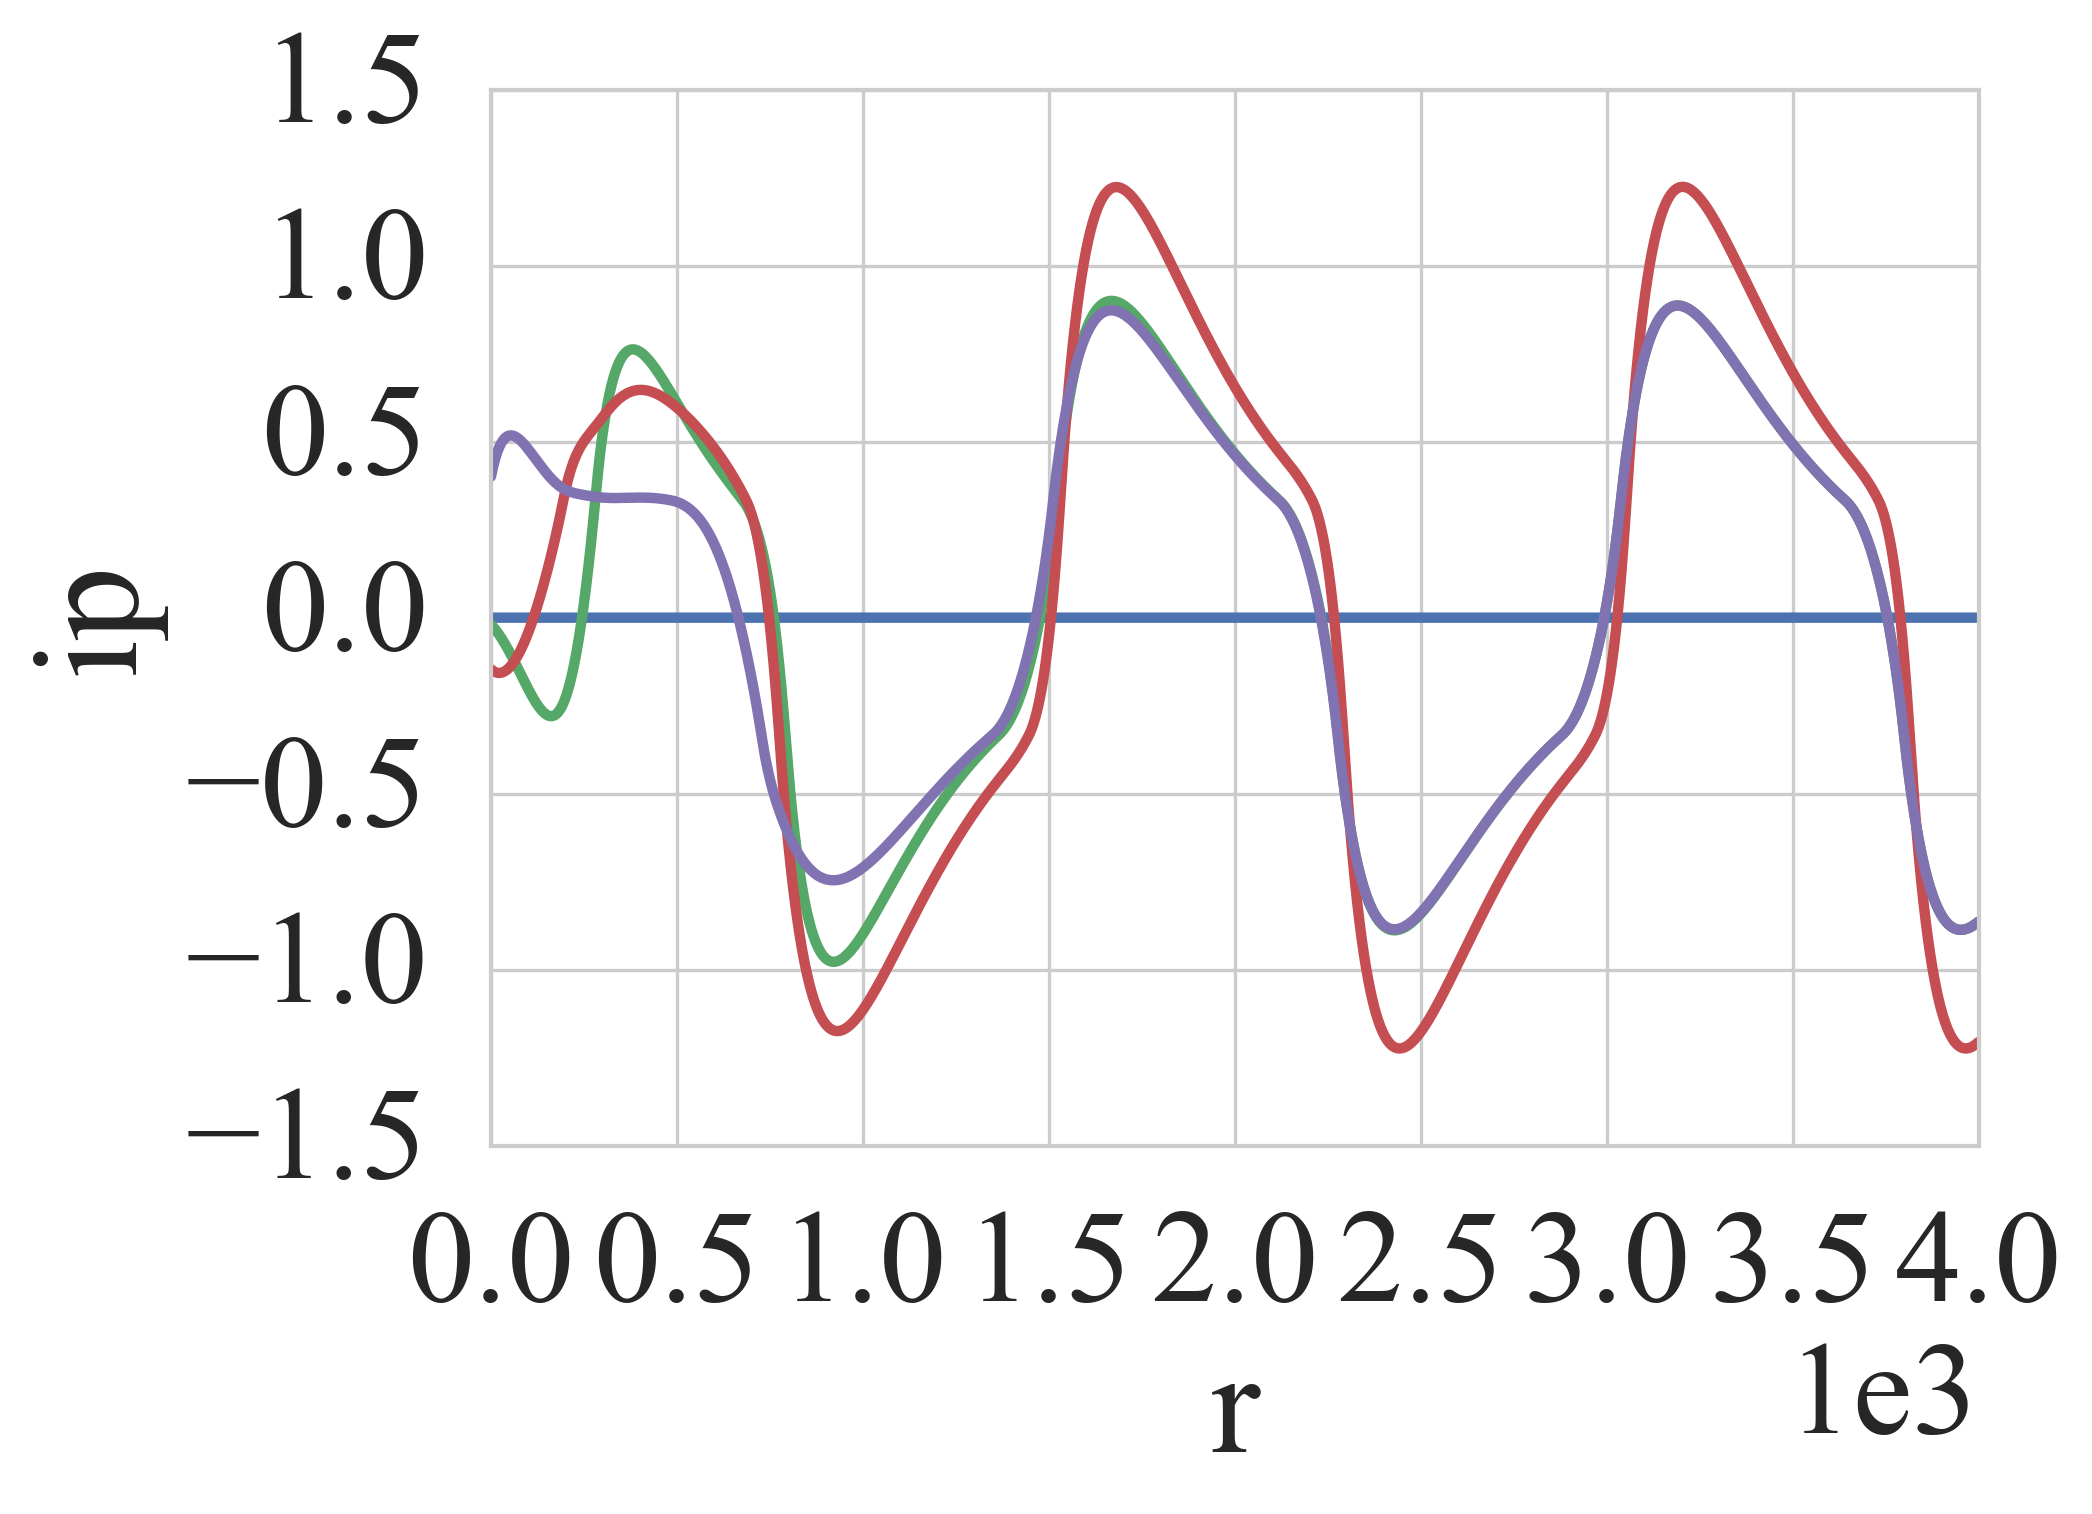
\includegraphics[width=0.4\linewidth,keepaspectratio]{./simulation/path/path_5_ip.png}\label{fig:path_5_ip}}\qquad
			\subfloat[][Period $T \approx 1522$ rounds.]{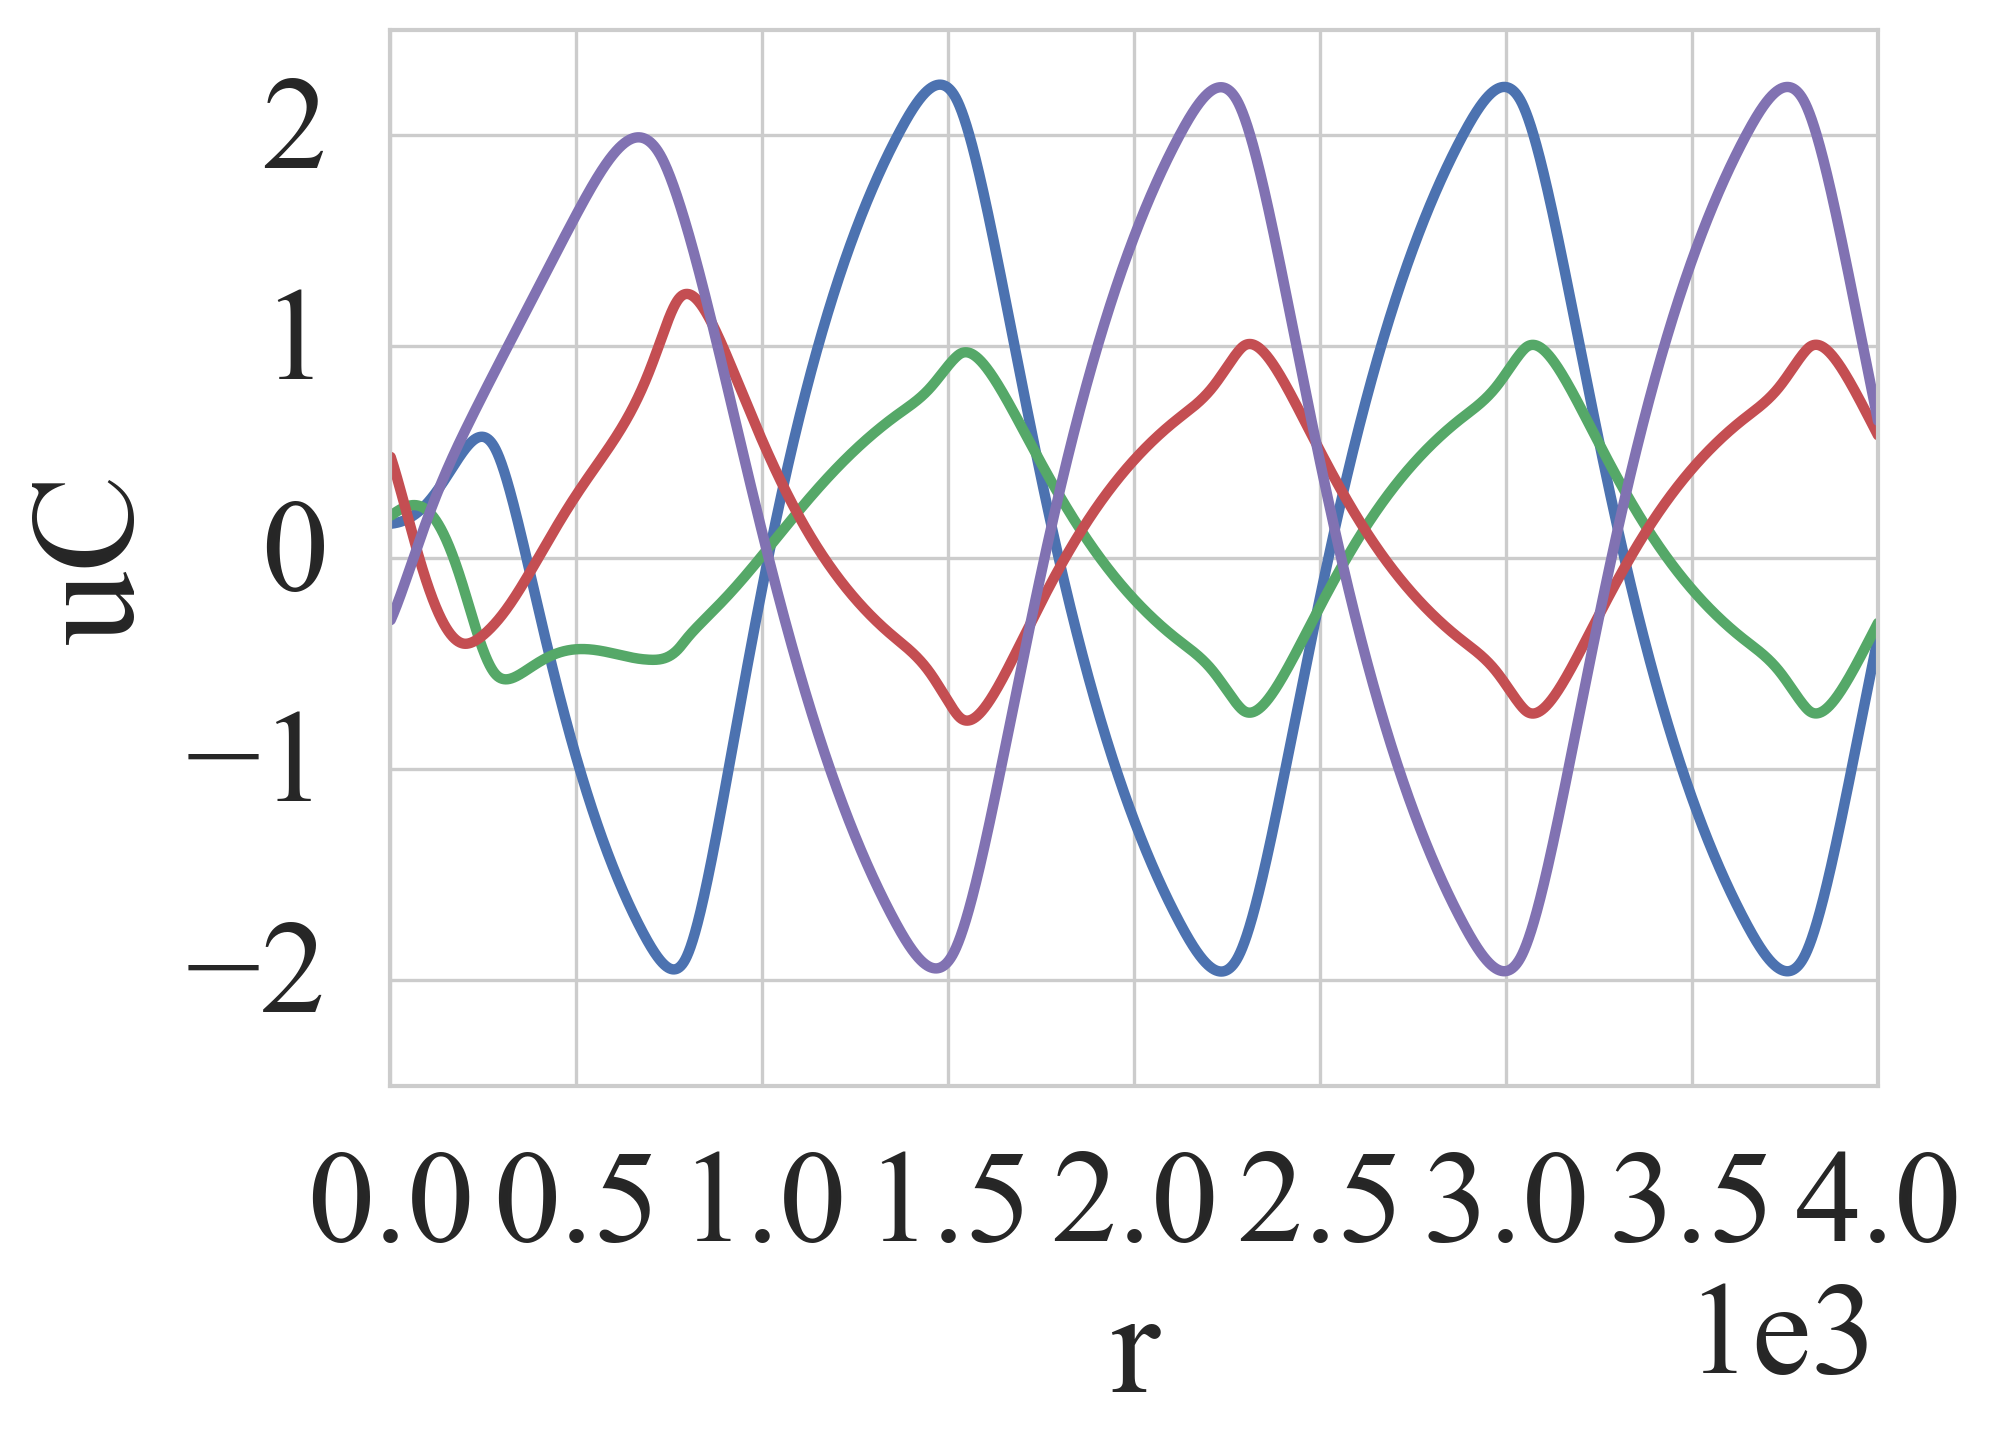
\includegraphics[width=0.4\linewidth,keepaspectratio]{./simulation/path/path_5_uC.png}\label{fig:path_5_uC}}
			
			\caption[Simulation - Paths]{Various paths of \Pes.}
			\label{fig:paths}
		\end{figure}

		\FloatBarrier

	\subsection{Trees of Physarum Elements}
		
		Let us study trees of \Pes next. The situation is similar to paths, with the added possibility of flows splitting up non-trivially at nodes of degree $3$. \Fref{fig:tree_6_graph} depicts a tree rooted at node $0$. We stress that the special status of root node exists only in the picture serving for better illustration. From the viewpoint of the model, all nodes are equal and the orientation of the edges matters not due to the symmetry of \Pes. As before \Fref{fig:tree_6_graph_legend} defines a color coding which serves as a legend for the plots of \Fref{fig:tree}.

		Similar to the study of paths, we find that a \Pn with a tree topology does not converge, see the capacitor voltages in \Fref{fig:tree_6_uC}. Again we observe periodic behavior for both currents and capacitor voltages with a period of $T \approx 1701$ rounds. Of particular interest is the behavior of the currents as given by \Fref{fig:tree_6_ip}. After a brief period of interaction, the tree exhibits perfect anti-phase oscillation between its subtrees. Looking at the edges $e_1 = (0,1)$ and $e_2 = (0,2)$ we see that whenever a positive current flows along $e_1$ an equal current with opposite sign flows through $e_2$. The same phase shift can be observed for the subtrees rooted at node $1$ and node $2$ respectively. This exact type of behavior was observed in $100$ independent simulations with different initial conditions.

		With regards to the period we observe identical values across all $100$ runs. Similar to the path, the period of the tree is robust to varying initial condition given the range we tested. A proof solidifying this statement is missing at this point.

		Let us discuss the behavior of the phases. Note that with respect to \Fref{fig:tree_6_graph} we may state that the currents through the left and the right subtree oscillate in perfect anti-phase. It is striking that the circuit itself suggest that it be viewed as a tree rooted at node $0$. It is not clear why it is precisely the subtrees at node $0$ that show this anti-phase entrainment. In principle we could choose any other node as the root, leading to different subtrees that should show different behavior. To shed light on these observations further numerical studies of various tree layouts could be useful.

		\begin{figure}
			\centering
			\subfloat[][]{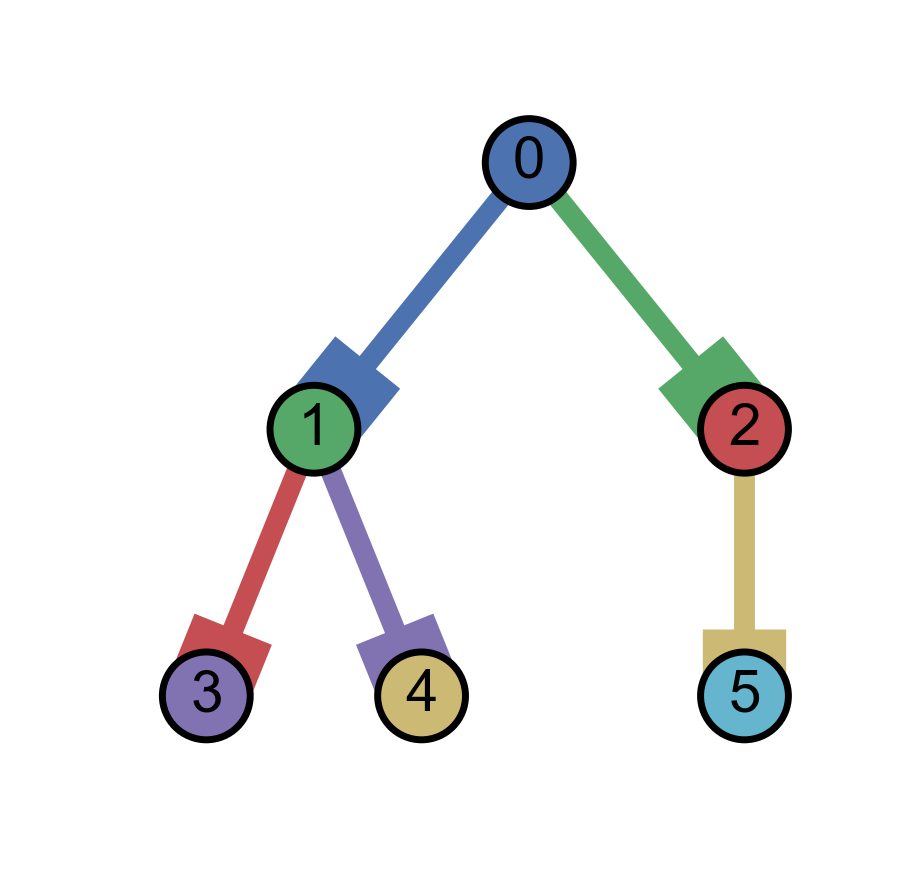
\includegraphics[width=0.4\linewidth,keepaspectratio,trim={0 2cm 0 2cm},clip]{./simulation/tree/tree_6.png}\label{fig:tree_6_graph}}\qquad
			\subfloat[][]{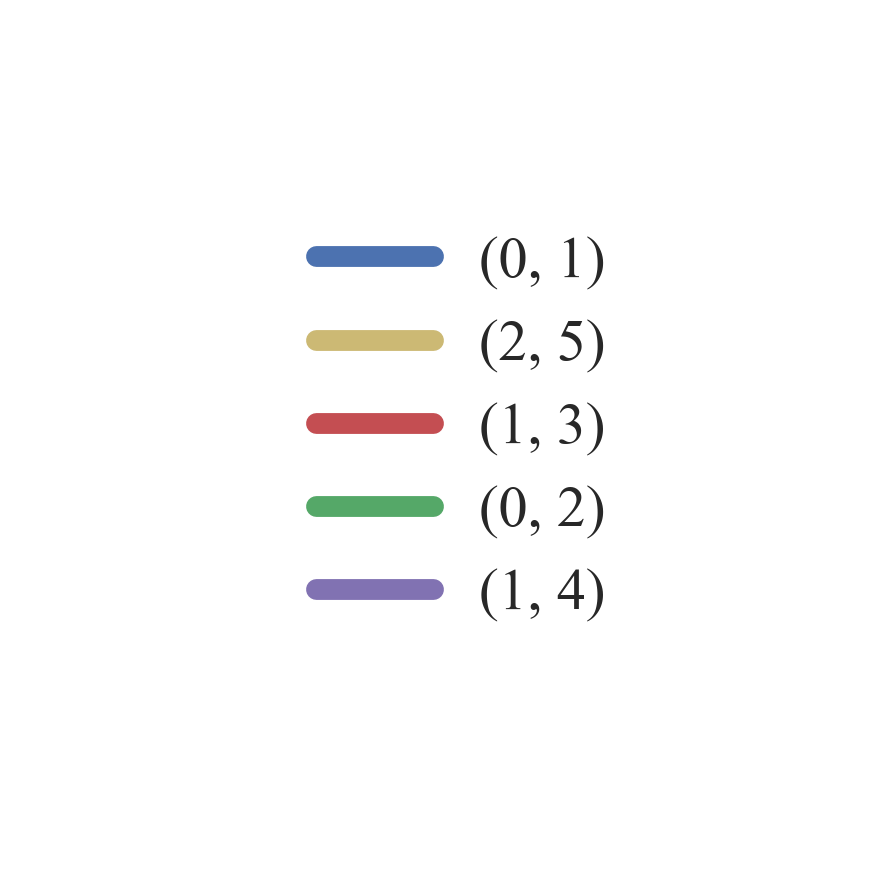
\includegraphics[width=0.4\linewidth,keepaspectratio,trim={0 2cm 0 2cm},clip]{./simulation/tree/tree_6_legend.png}\label{fig:tree_6_graph_legend}}
			\newline
			\subfloat[][]{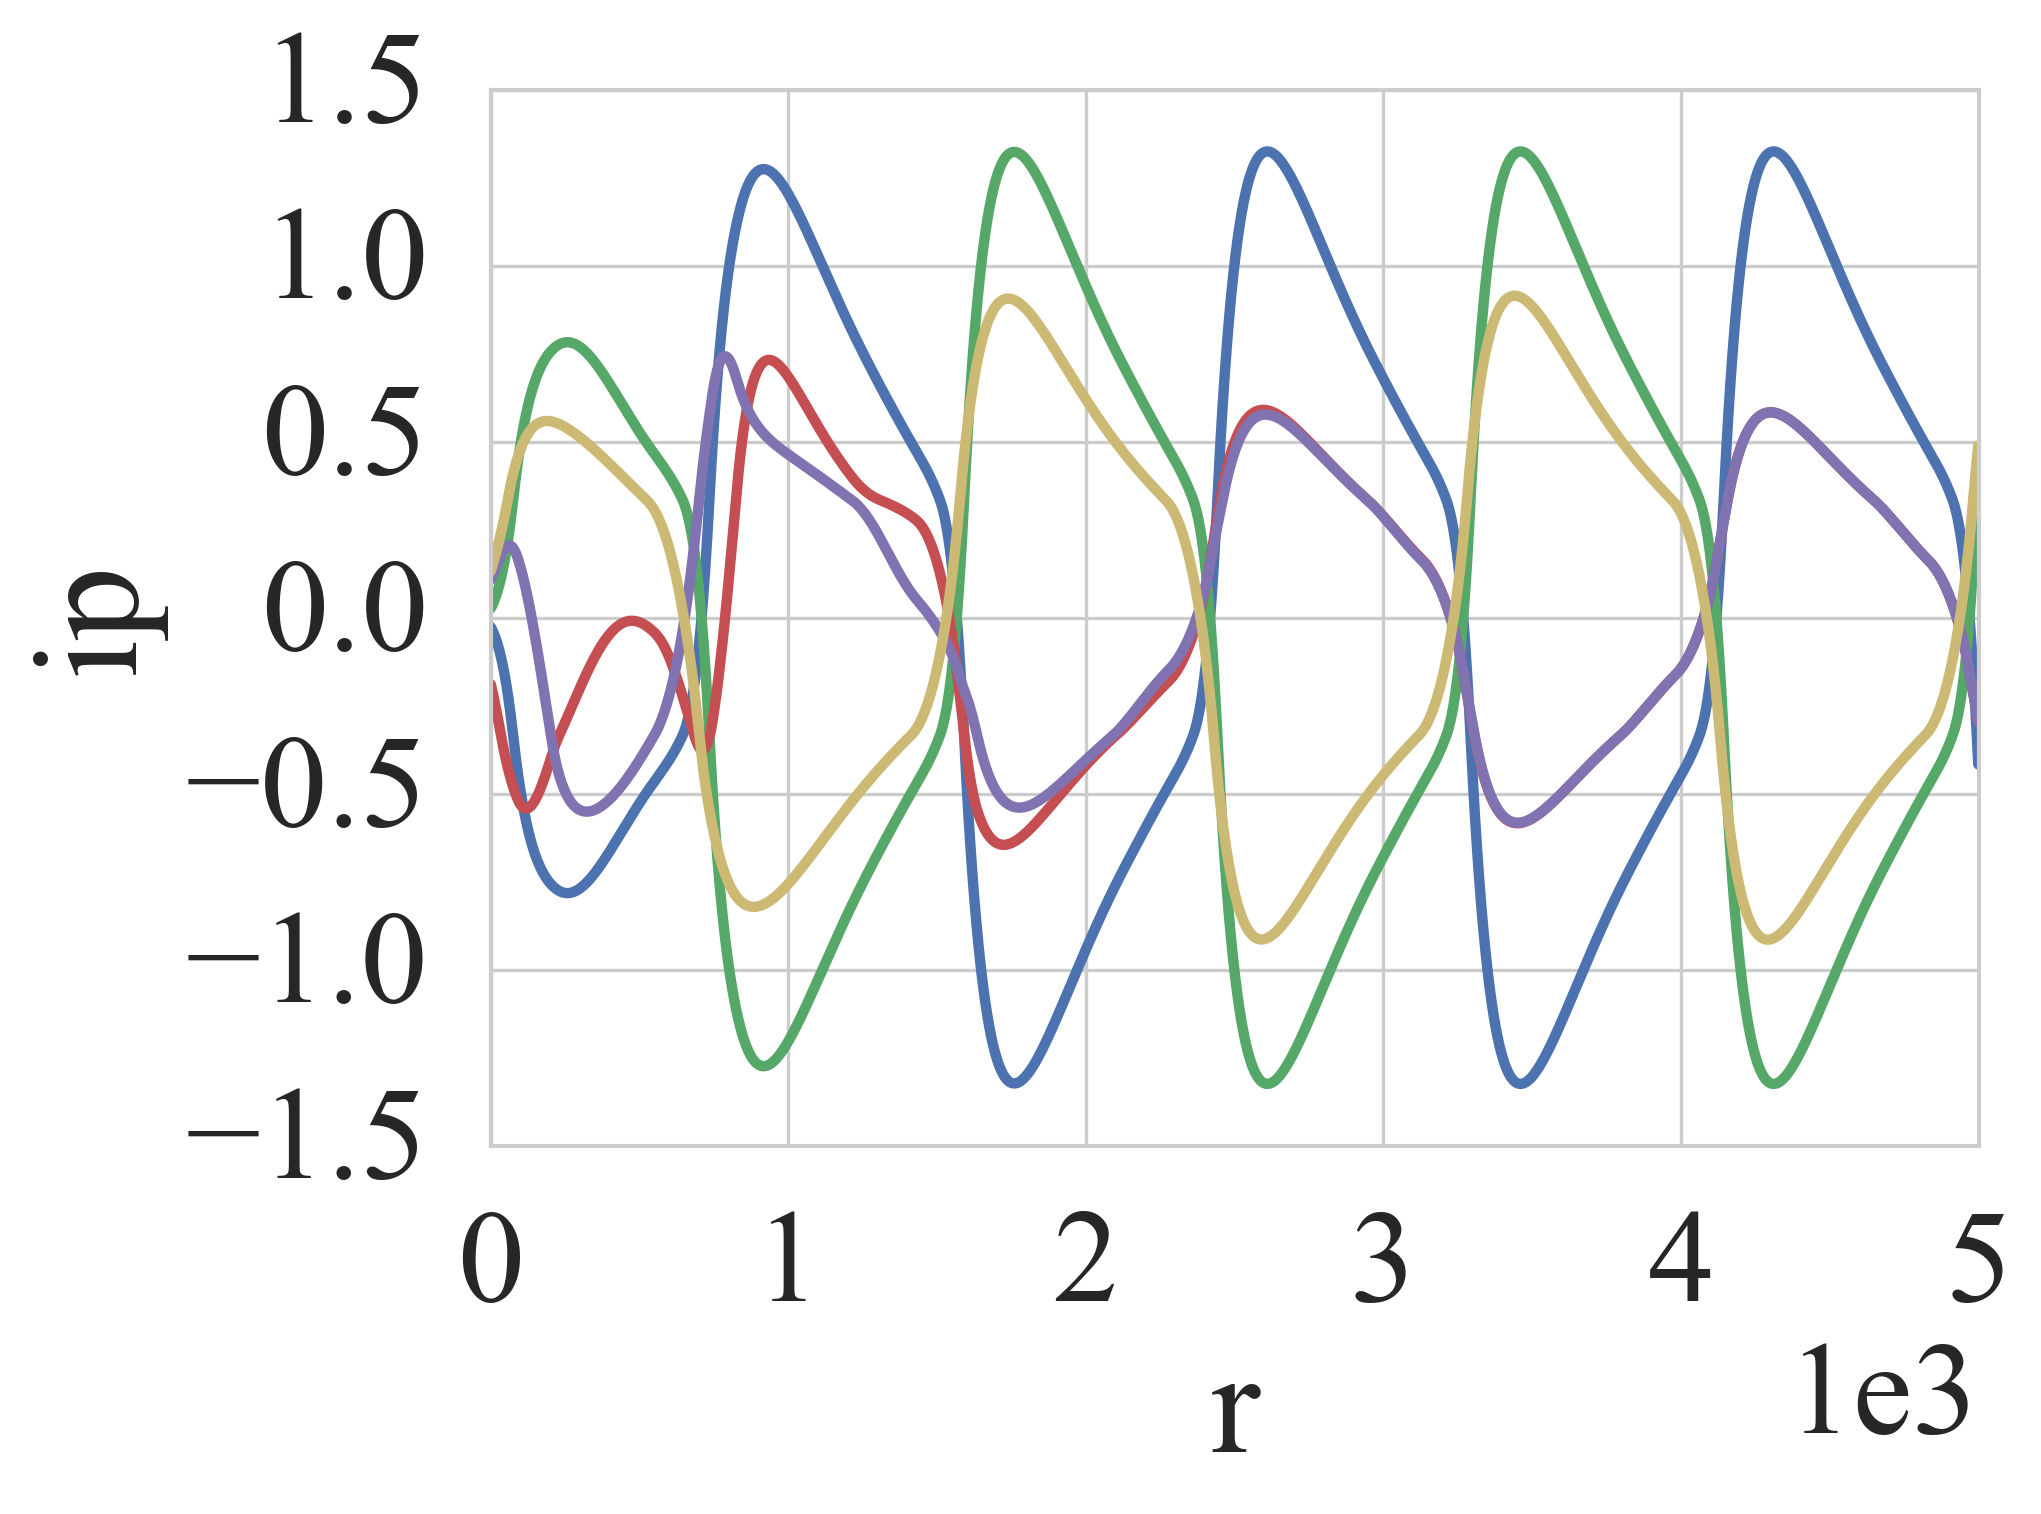
\includegraphics[width=0.4\linewidth,keepaspectratio]{./simulation/tree/tree_6_ip.png}\label{fig:tree_6_ip}}\qquad
			\subfloat[][]{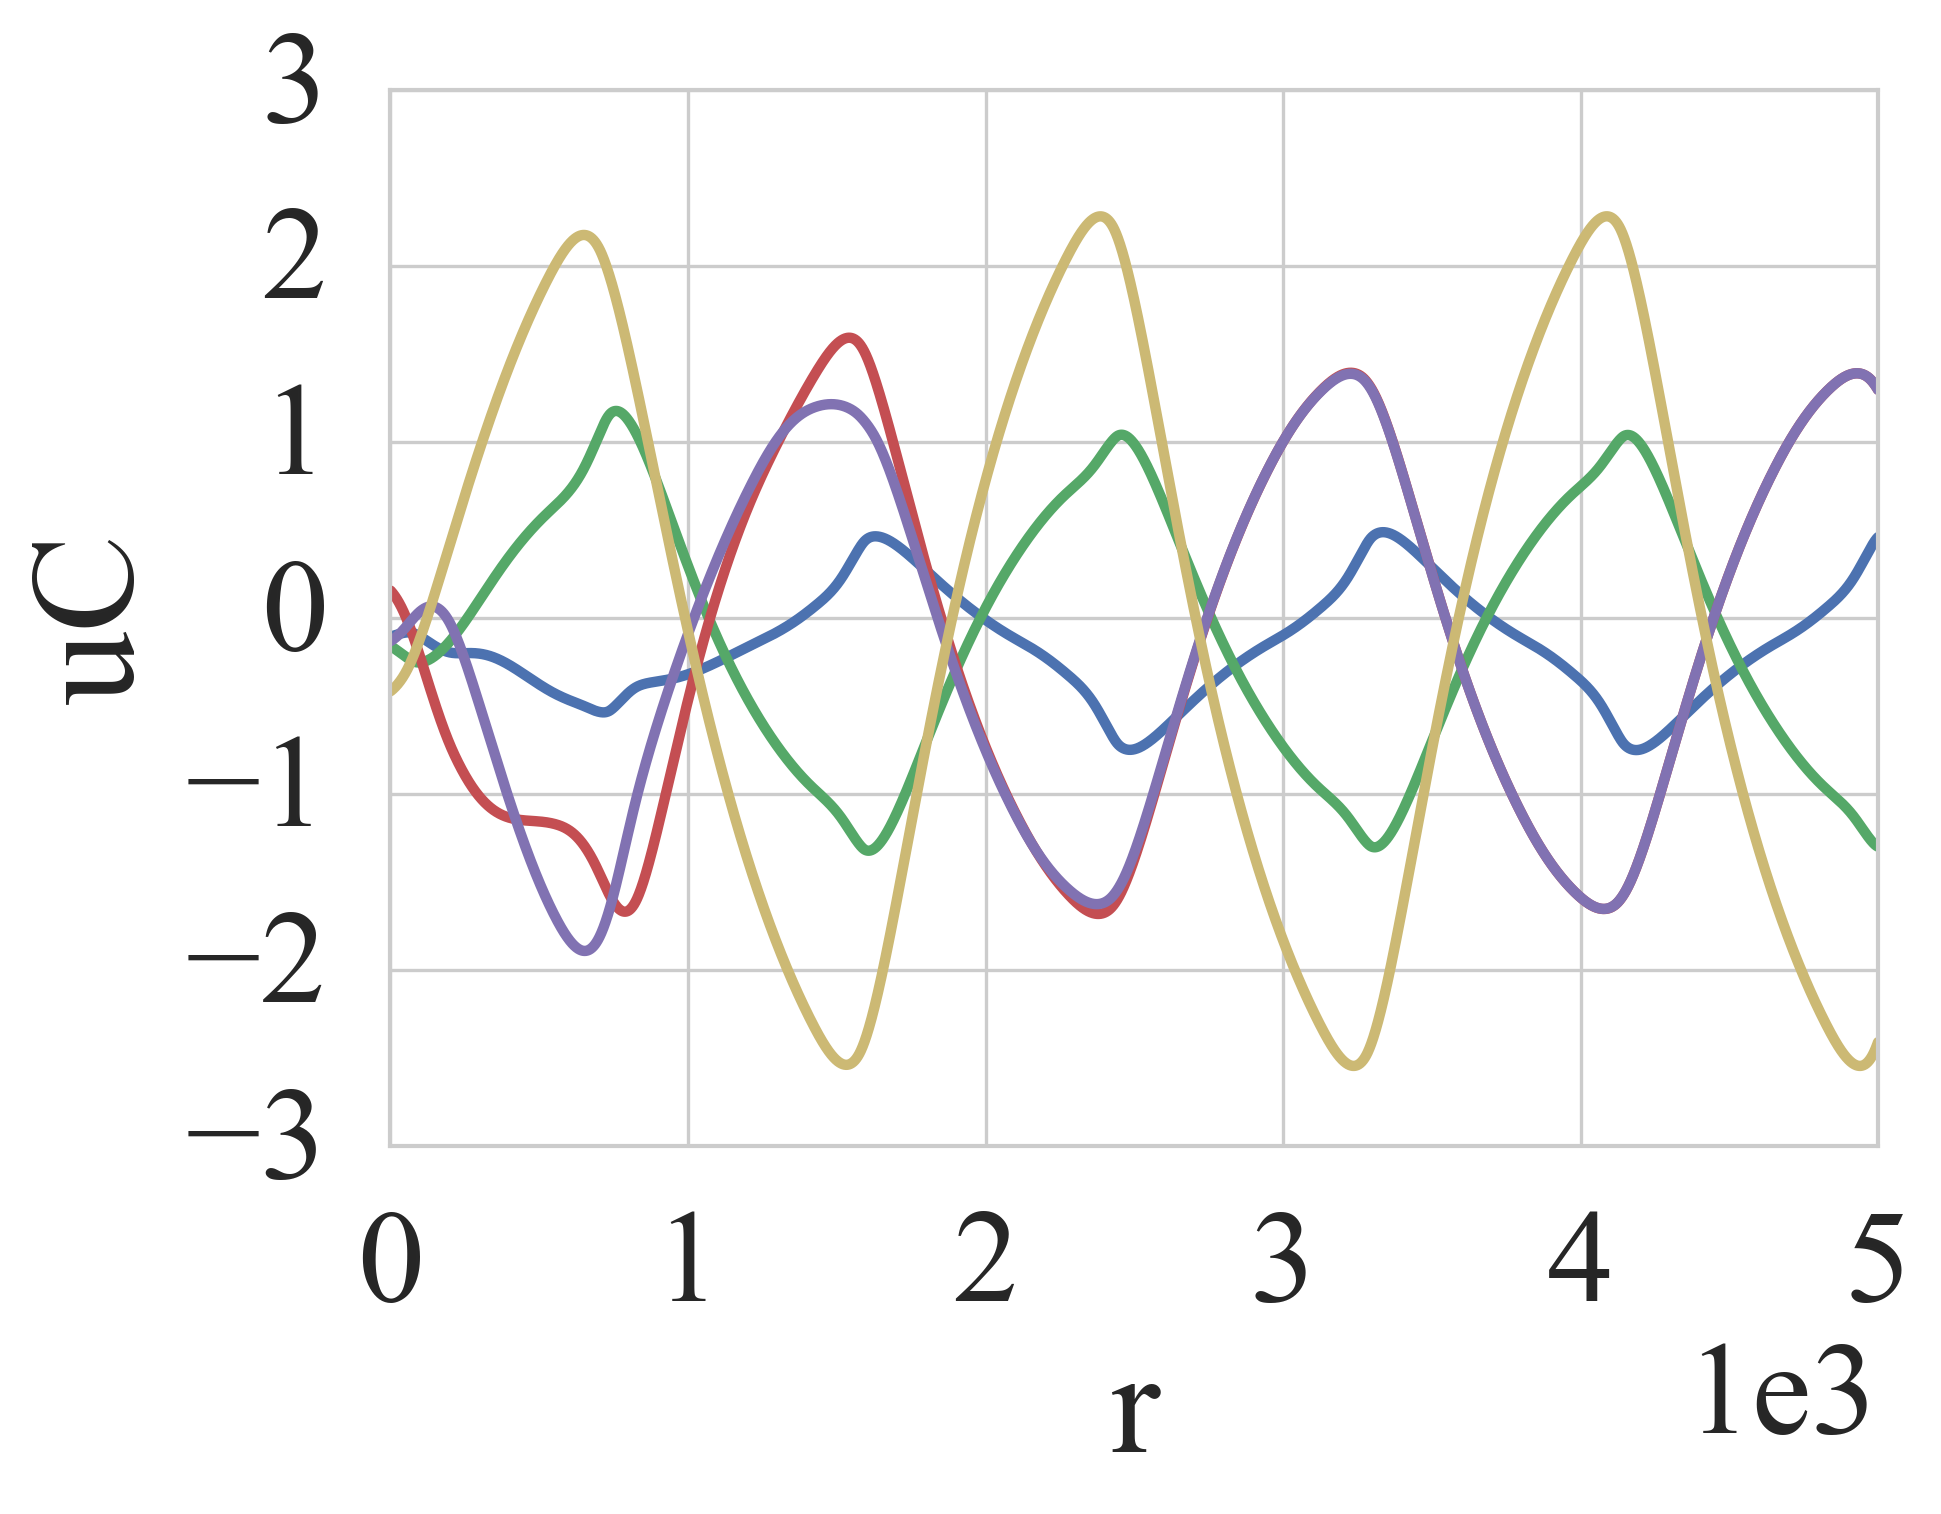
\includegraphics[width=0.4\linewidth,keepaspectratio]{./simulation/tree/tree_6_uC.png}\label{fig:tree_6_uC}}
			
					
			\caption[Simulation - Trees]{A simple tree of \Pes.}
			\label{fig:tree}
		\end{figure}

	\subsection{Two Linked Cycles of Physarum Elements}

		Finally, we combine the features of paths and cycles to obtain a \Pn as shown in \Fref{fig:dumbbell_graph}. \Fref{fig:dumbbell_graph_legend} defines a color coding which serves as a legend for the plots of \Fref{fig:dumbbell}.

		The proposed topology is meant as an first attempt of exploring the connection between the workings of our model and the behavior of live \P. We do so by interpreting the \Pn in \Fref{fig:dumbbell_graph} as an abstract representation of the way \P was modeled as a living system of delay-coupled mechanical oscillators as mentioned in the short survey of existing modeling approaches~\cite{PhysRevLett.85.2026}. See \Fref{sec:oscillator_experiment} for details. The two $3$-cycles represent the reservoirs while the path of length $1$ constitutes the channel connecting them. In the original wet-lab experiment \P showed rich self-synchronizing oscillation patterns between the distinct reservoirs with both in-phase and anti-phase entrainment. It is interesting to ask, whether our model can reproduce any of the observed effects.

		To explore the behavior of our model, we present $3$ distinct simulation instances. First we look towards the capacitor voltages to find symmetric oscillations in perfect anti-phase between the two cycles. After a brief period of entrainment, the edges of the two cycles converge symmetrically around the value the channel edges $(0,5)$ converges to, see \Fref{fig:dumbbell_3_1_uC_symmetric_positive}, \Fref{fig:dumbbell_uC_symmetric_negative} and \Fref{fig:dumbbell_uC_asymmetric}. The picture is similar to what was observed for the diamond graph, except that the non-bridge edges, \ie the cycle edges, can now sustain oscillation. While this anti-phase entrainment is reminiscent of the behavior delay-coupled oscillators, we were not able to get our model to show in-phase entrainment. In fact, given the invariants we were able to proof, it is unlikely to be possible.

		With regards to the currents flowing in the \Pn, we observe scenarios that are intuitive. The currents in both cycles can be identical and flowing in the same direction, either clockwise, see \Fref{fig:dumbbell_ip_symmetric_negative}, or counter-clockwise, see \Fref{fig:dumbbell_3_1_ip_symmetric_positive}. Furthermore, the currents can flow in the opposite directions adding two more scenarios. \Fref{fig:dumbbell_ip_asymmetric} shows one of them with the l.h.s.\ cycle showing counter-clockwise flow while the r.h.s.\ cycle exhibits clockwise flow. A scenario where currents are damped is not shown. In contrast to cycles, the coupling between the two cycles induces oscillations in the circular flows. Interesting in all scenarios, is the behavior of the channel edge $(0,5)$ which shows periodic flow reversals with a period of $T \approx 1629 $ rounds and large peak flows. Again $100$ repetitions of the simulation suggests the period to be independent on the initial conditions within the range we tested.

		Clearly, the model we propose yields only a crude approximation of the behavior of \P. Based on the high degree of abstraction and the relatively simple model, it is surprising that effects like flow reversal and anti-phase entrainment emerge naturally. It is also apparent, that we are limited to simple topologies of \Pes if we are to make sense of the behavior analytically. Of course this does not prohibit using the model as a black box for more complicated and/or larger graphs.


		\begin{figure}
			\centering
			\subfloat[][]{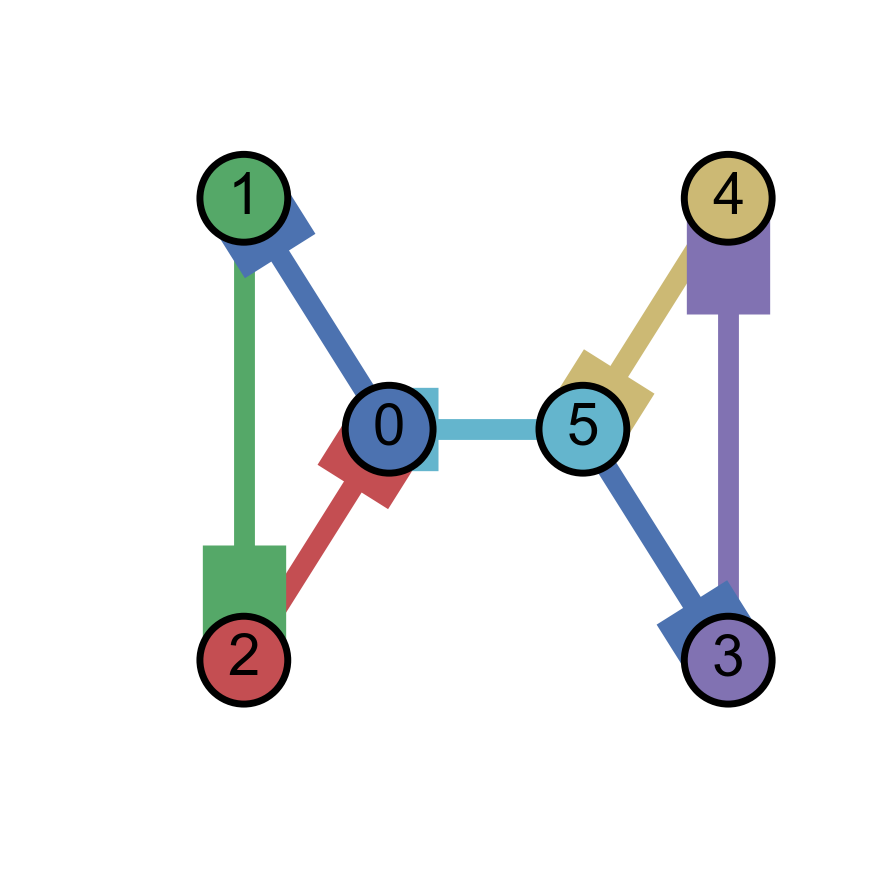
\includegraphics[width=0.35\linewidth,keepaspectratio,trim={0 4cm 0 3cm},clip]{./simulation/dumbbell/dumbbell_3_1.png}\label{fig:dumbbell_graph}}\qquad
			\subfloat[][]{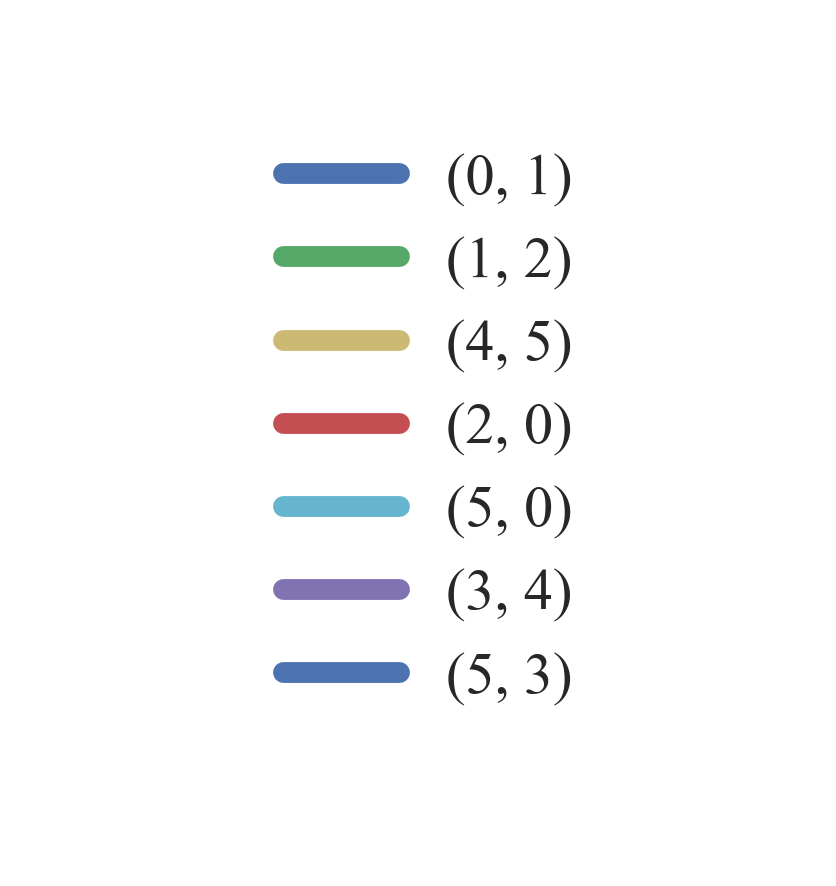
\includegraphics[width=0.35\linewidth,keepaspectratio,trim={0 4cm 0 3cm},clip]{./simulation/dumbbell/dumbbell_3_1_legend.png}\label{fig:dumbbell_graph_legend}}
			\newline
			\subfloat[][]{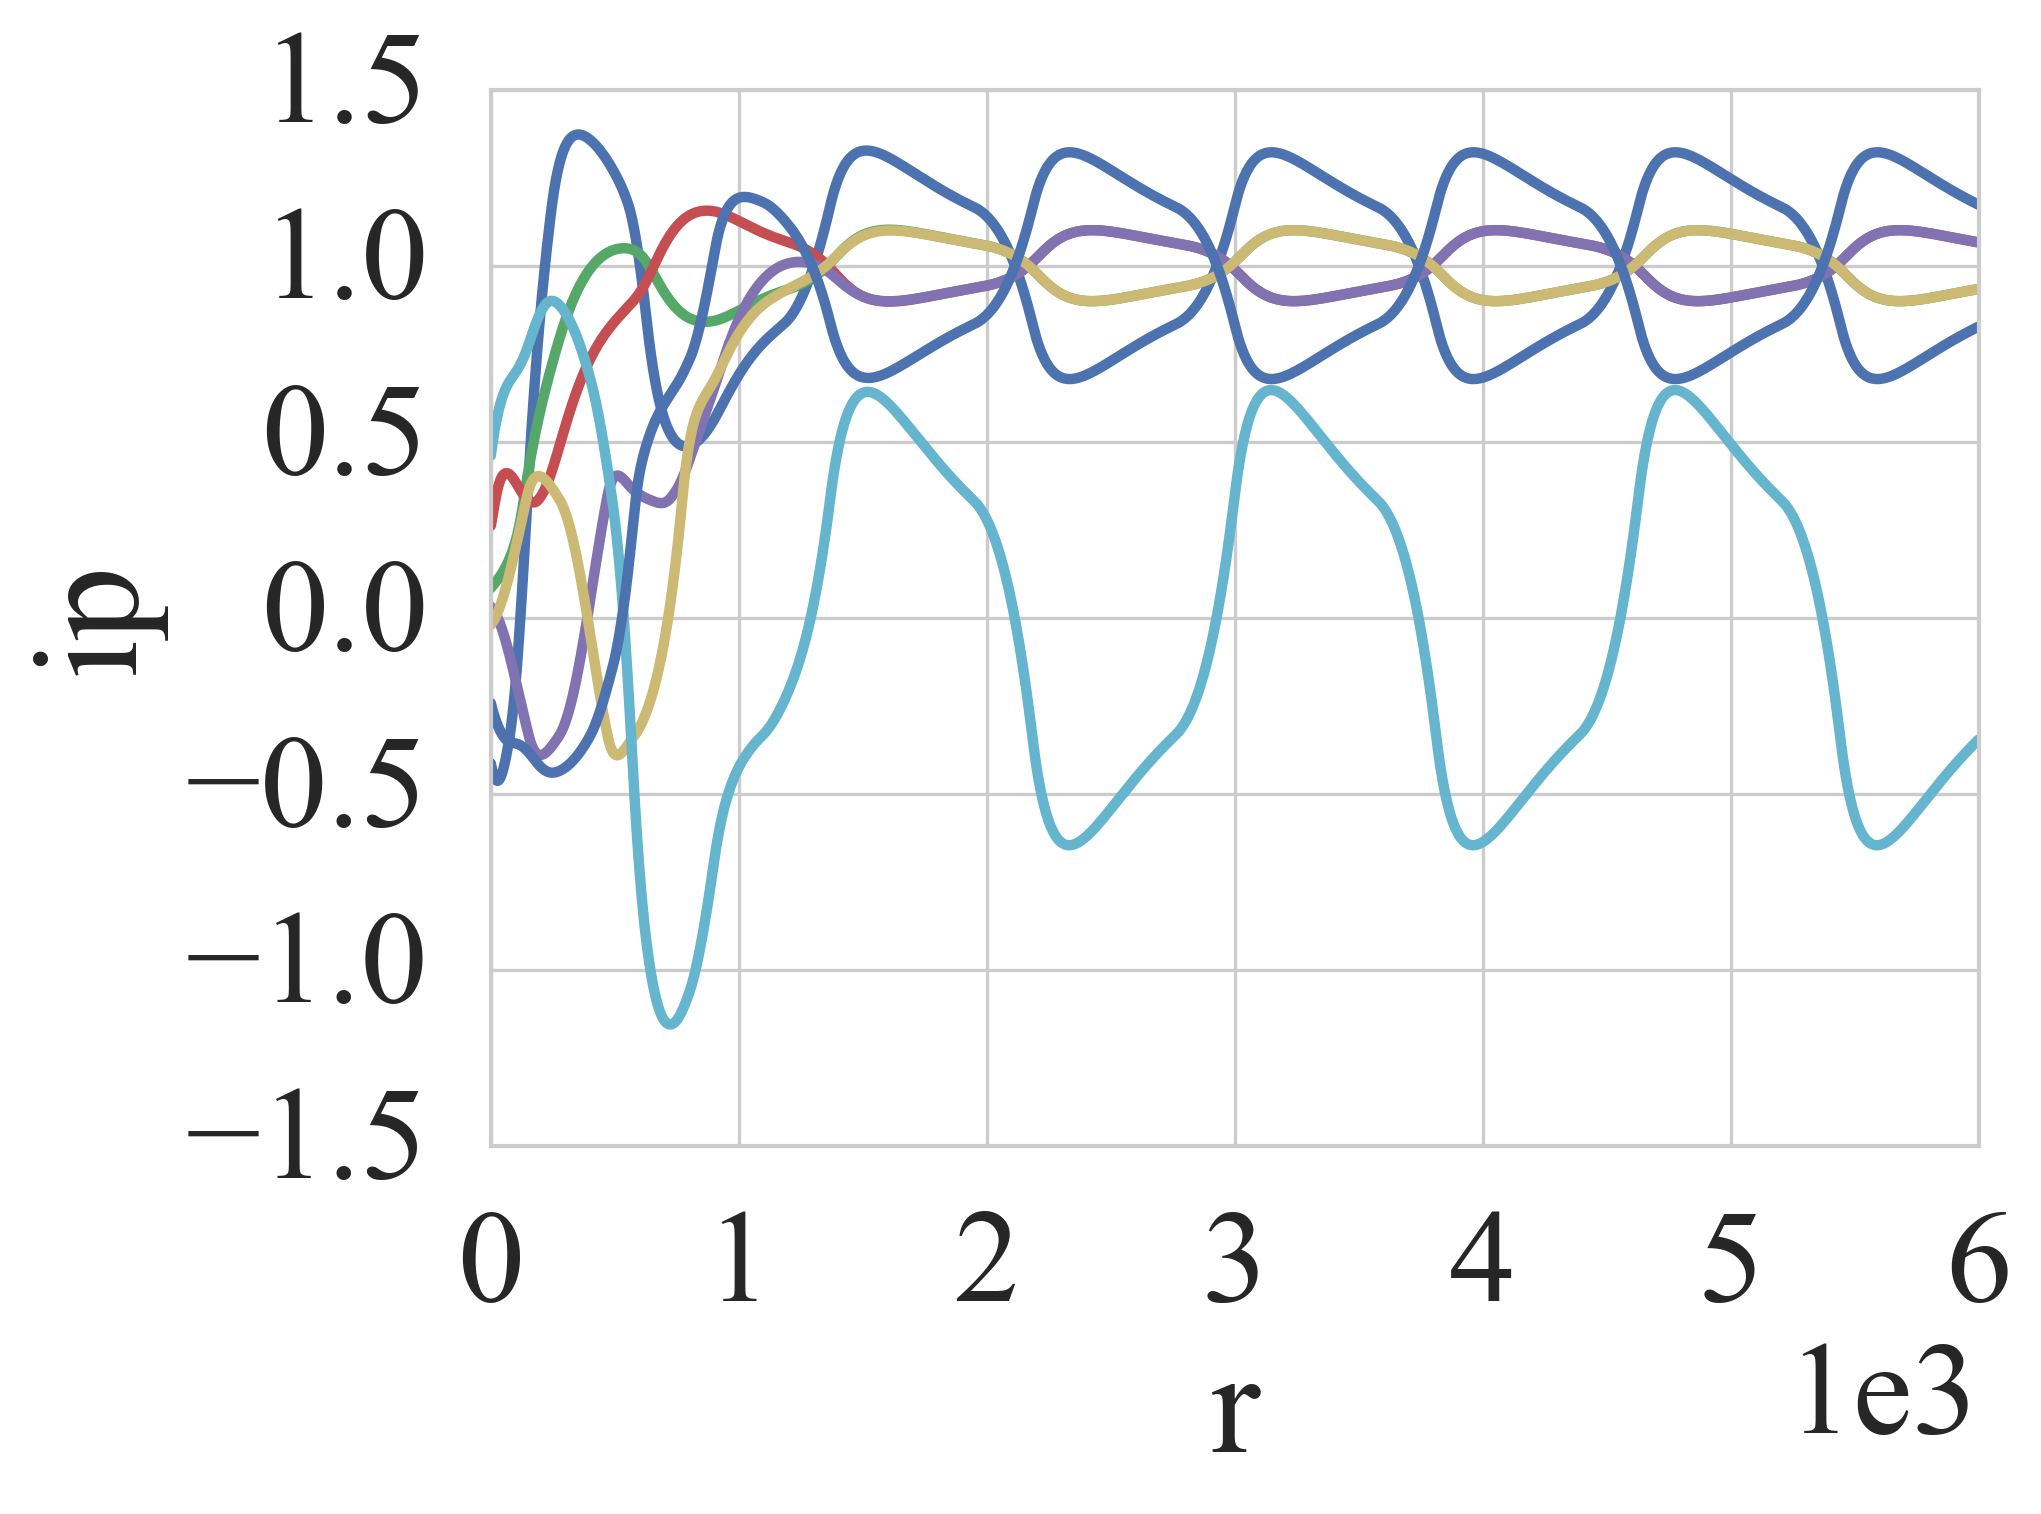
\includegraphics[width=0.4\linewidth,keepaspectratio]{./simulation/dumbbell/dumbbell_3_1_ip_symmetric_positive.png}\label{fig:dumbbell_3_1_ip_symmetric_positive}}\qquad
			\subfloat[][]{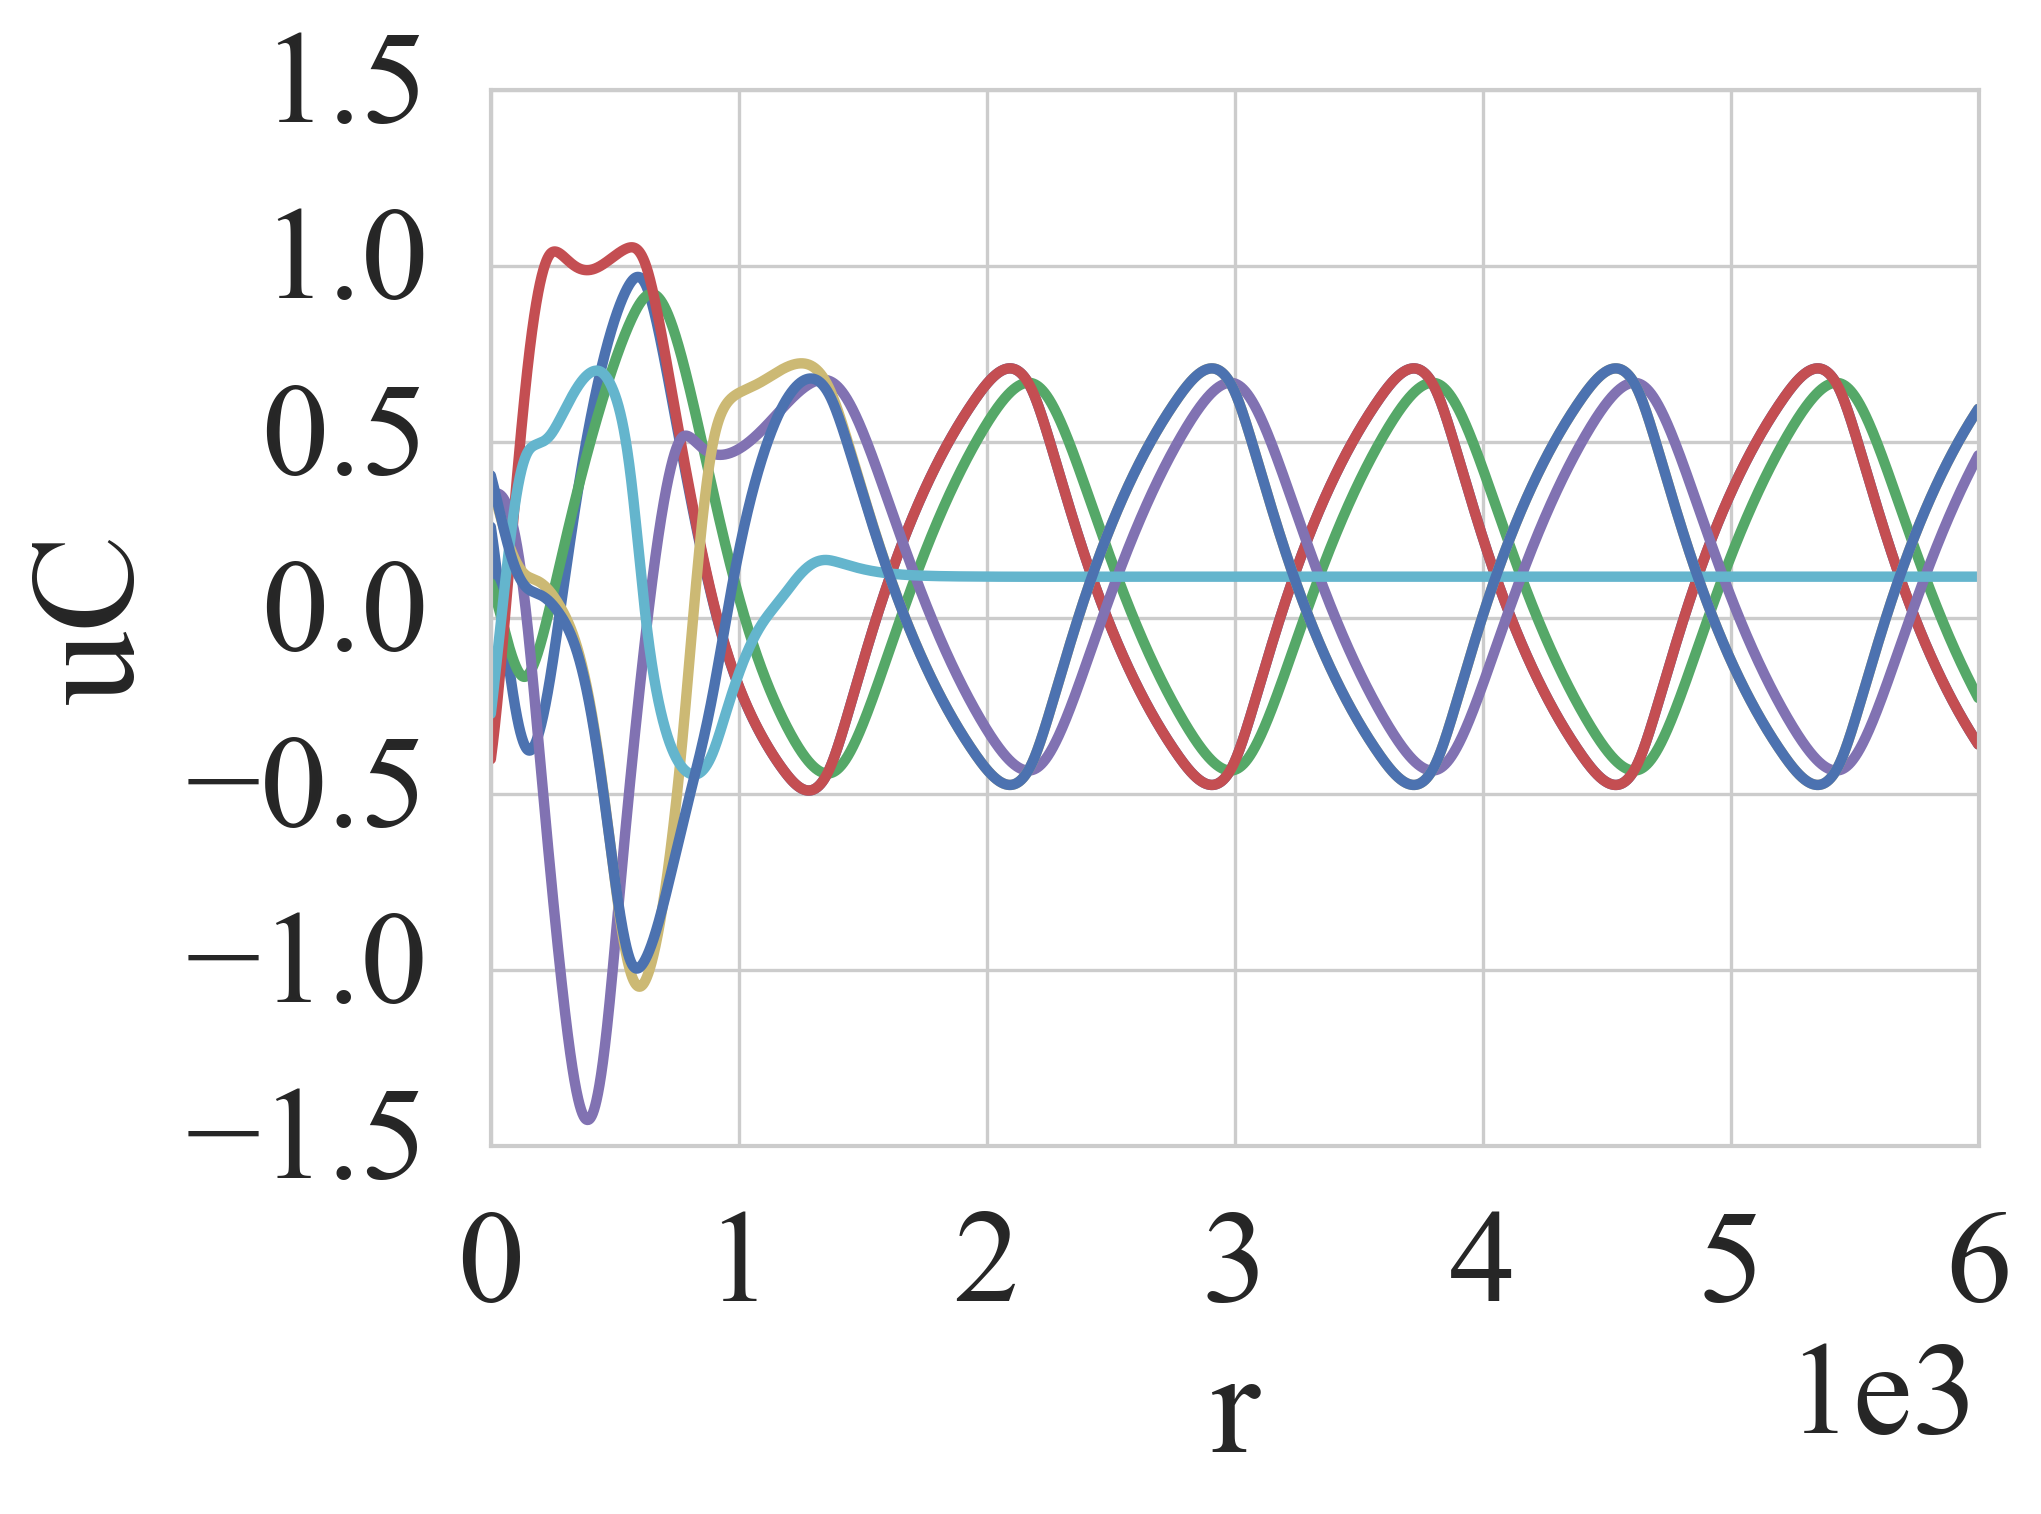
\includegraphics[width=0.4\linewidth,keepaspectratio]{./simulation/dumbbell/dumbbell_3_1_uC_symmetric_positive.png}\label{fig:dumbbell_3_1_uC_symmetric_positive}}
			\newline
			\subfloat[][]{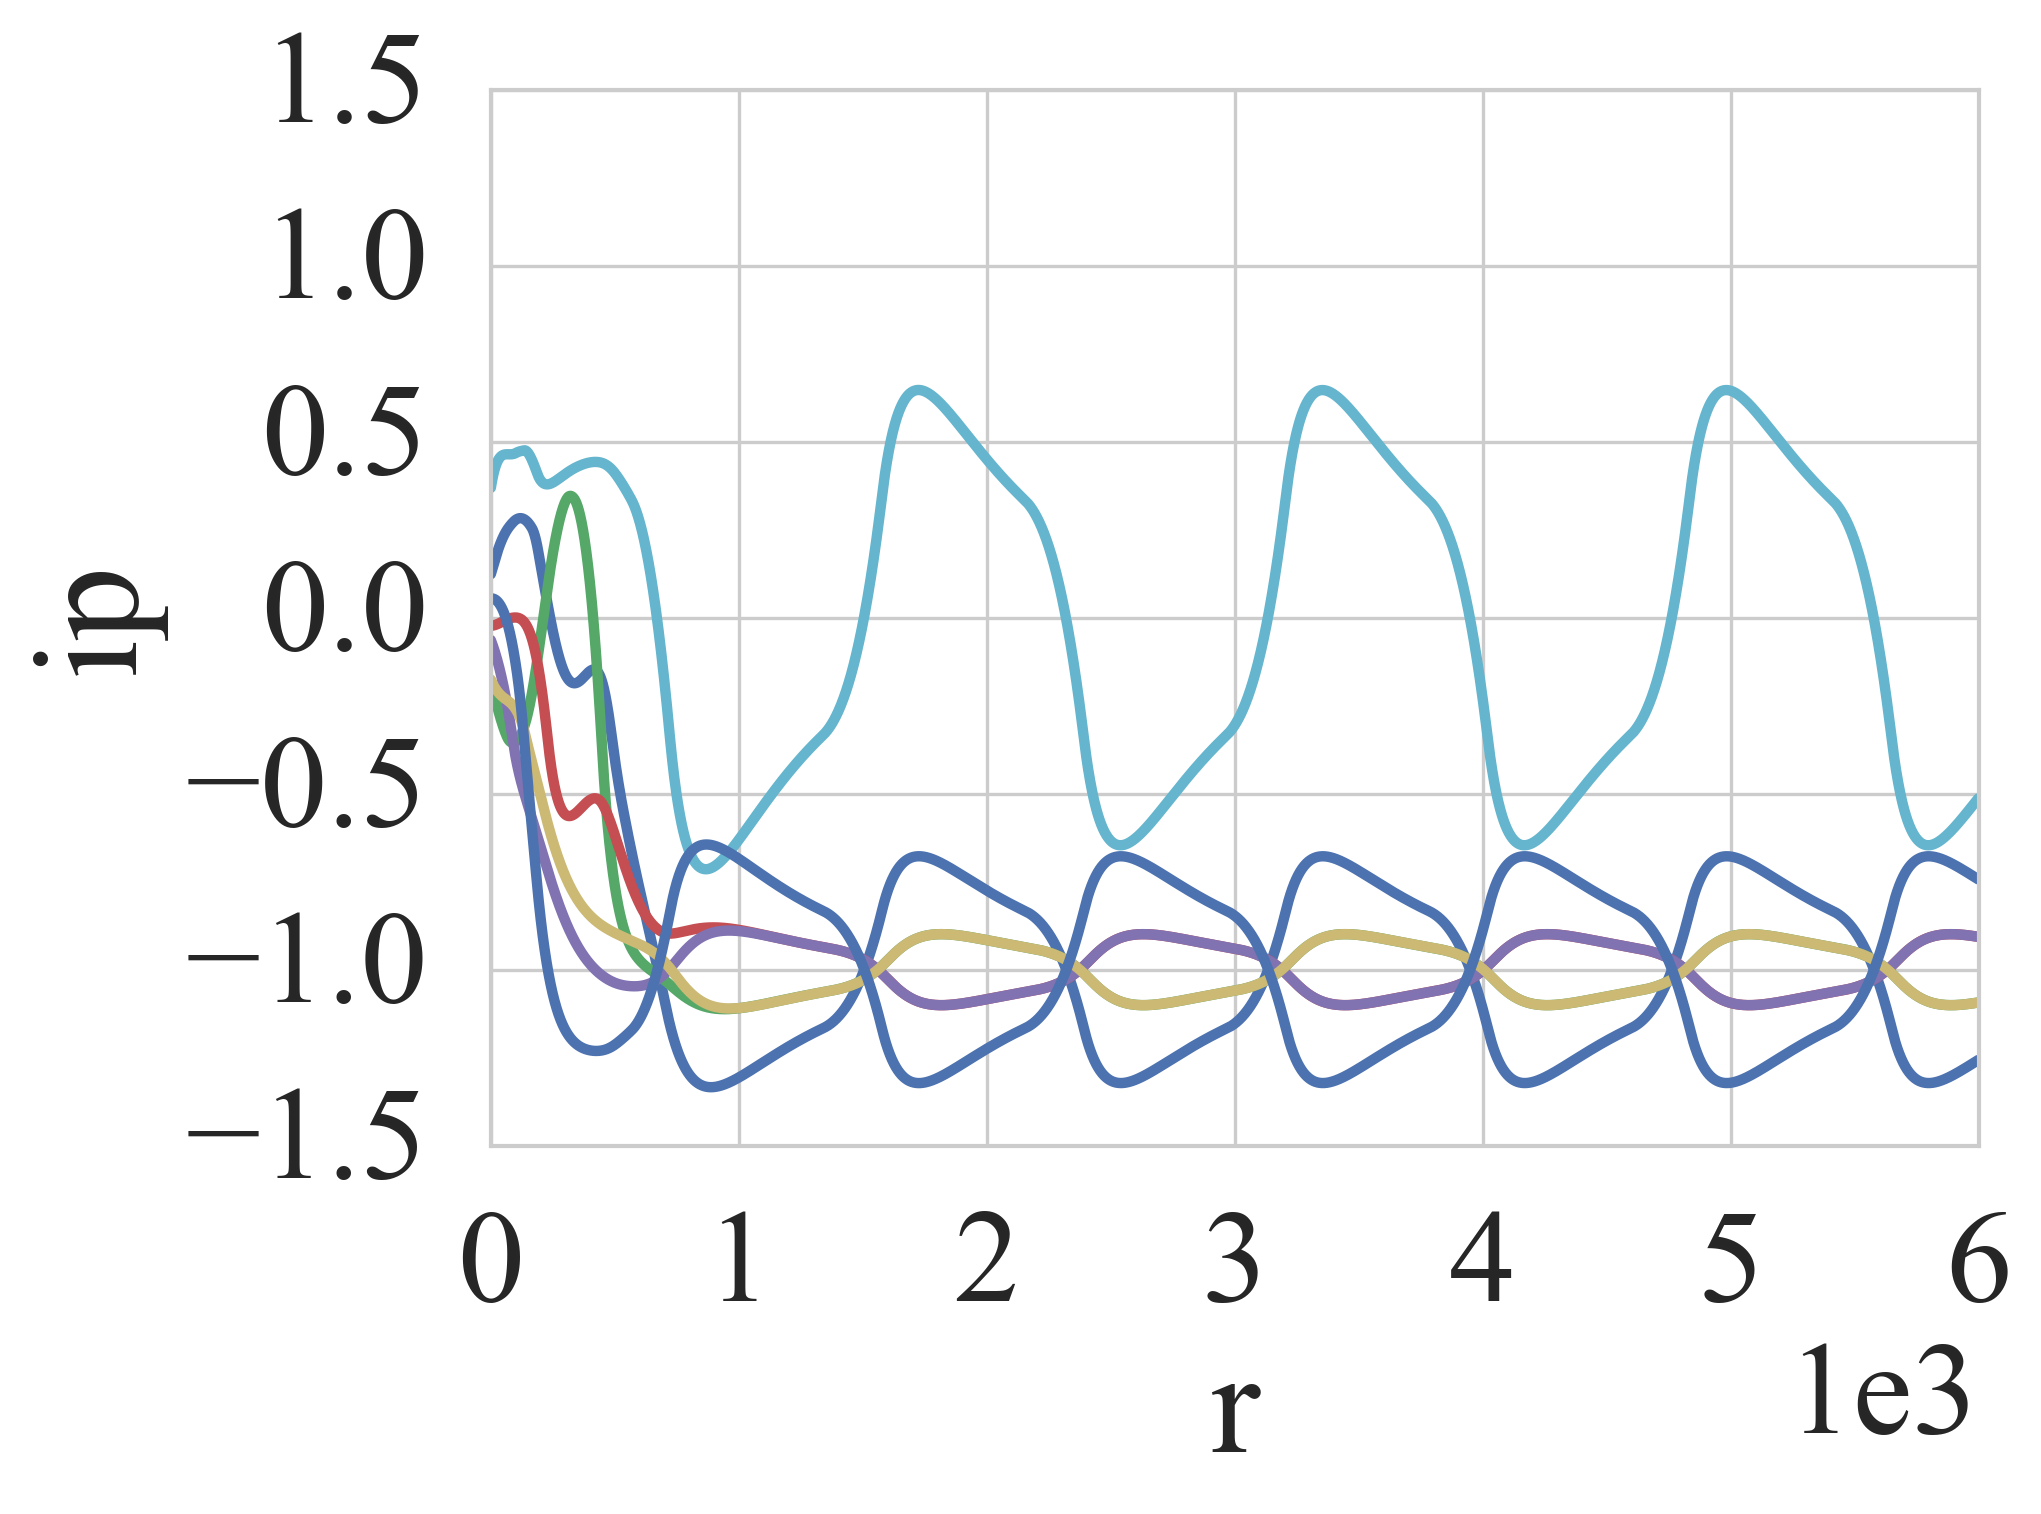
\includegraphics[width=0.4\linewidth,keepaspectratio]{./simulation/dumbbell/dumbbell_3_1_ip_symmetric_negative.png}\label{fig:dumbbell_ip_symmetric_negative}}\qquad
			\subfloat[][]{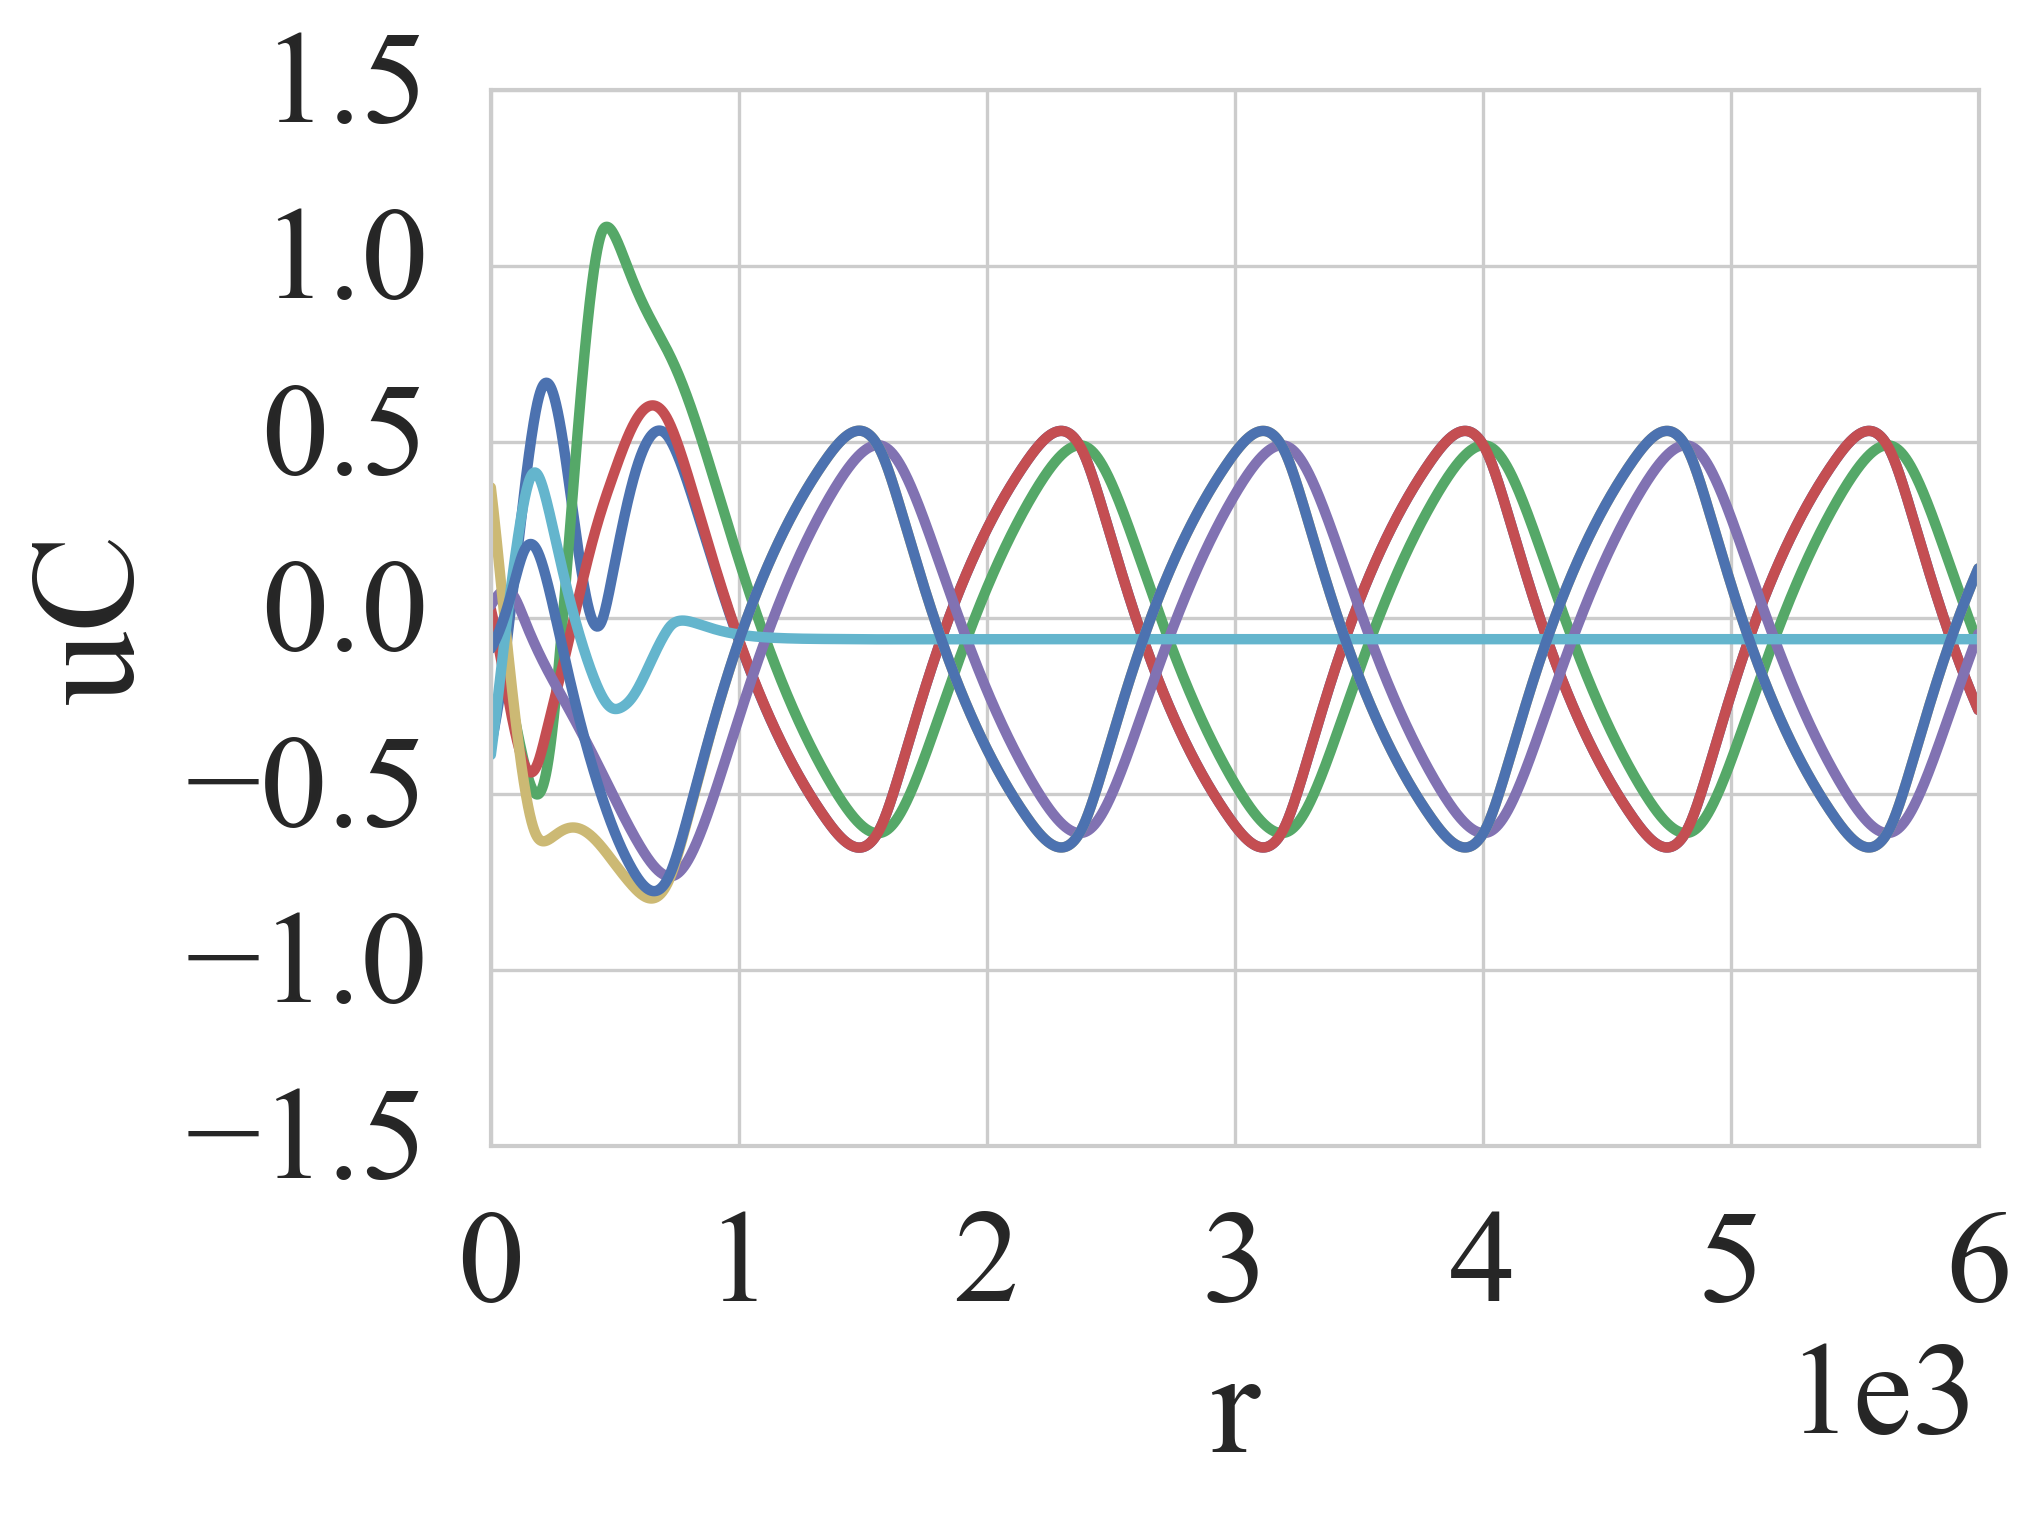
\includegraphics[width=0.4\linewidth,keepaspectratio]{./simulation/dumbbell/dumbbell_3_1_uC_symmetric_negative.png}\label{fig:dumbbell_uC_symmetric_negative}}
			\newline
			\subfloat[][]{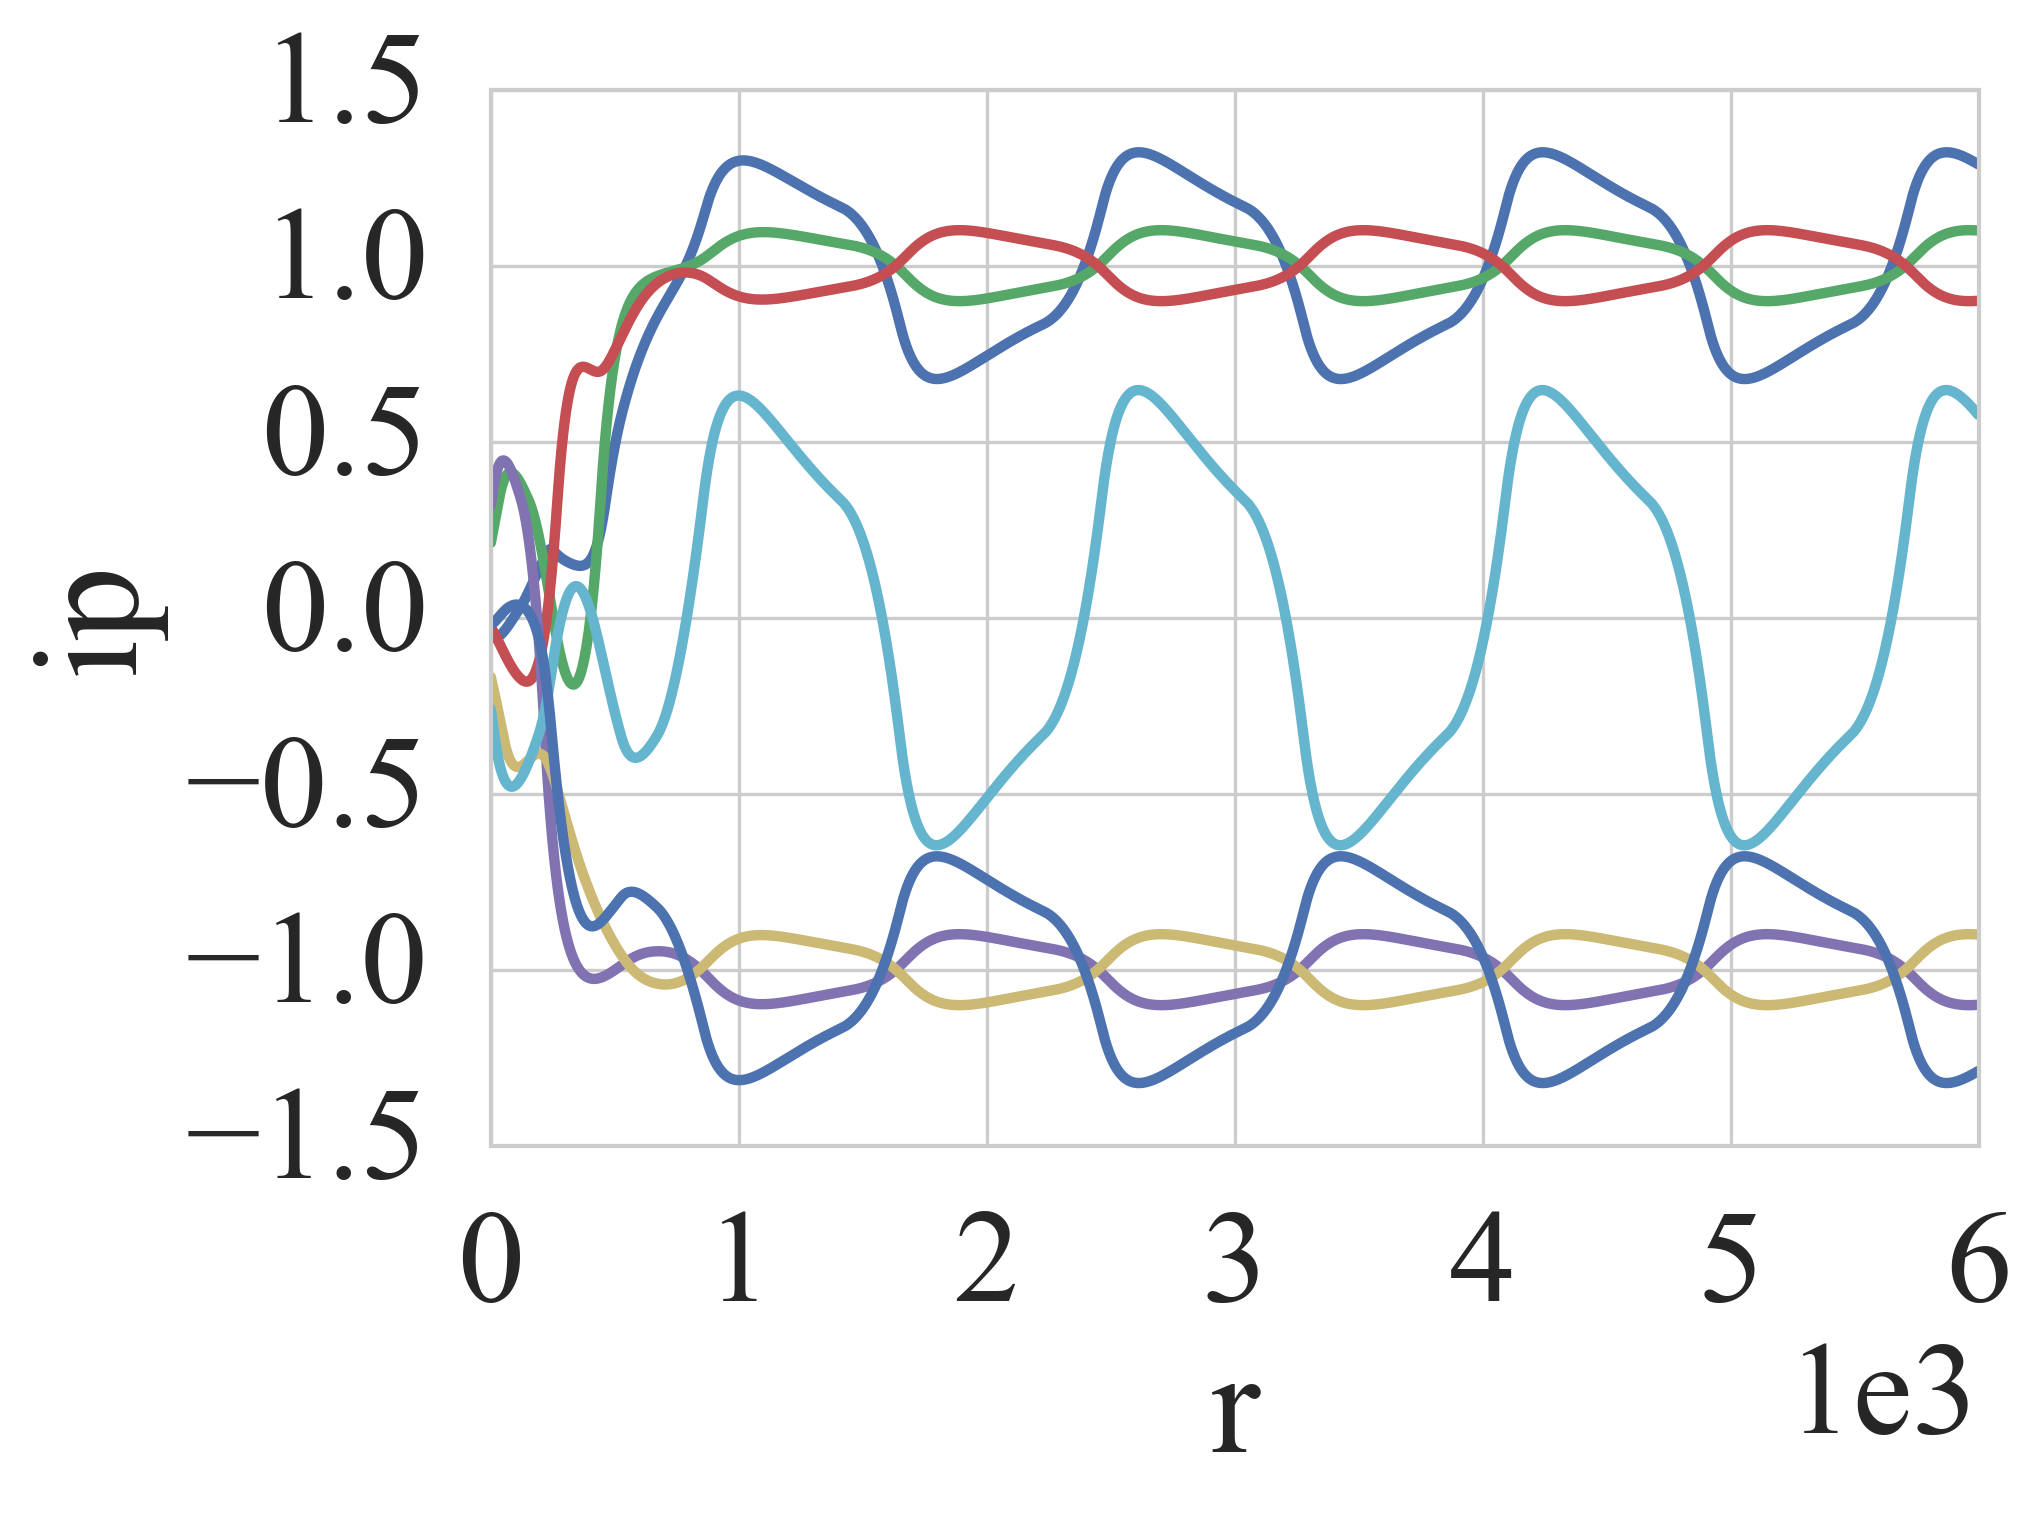
\includegraphics[width=0.4\linewidth,keepaspectratio]{./simulation/dumbbell/dumbbell_3_1_ip_asymmetric.png}\label{fig:dumbbell_ip_asymmetric}}\qquad
			\subfloat[][]{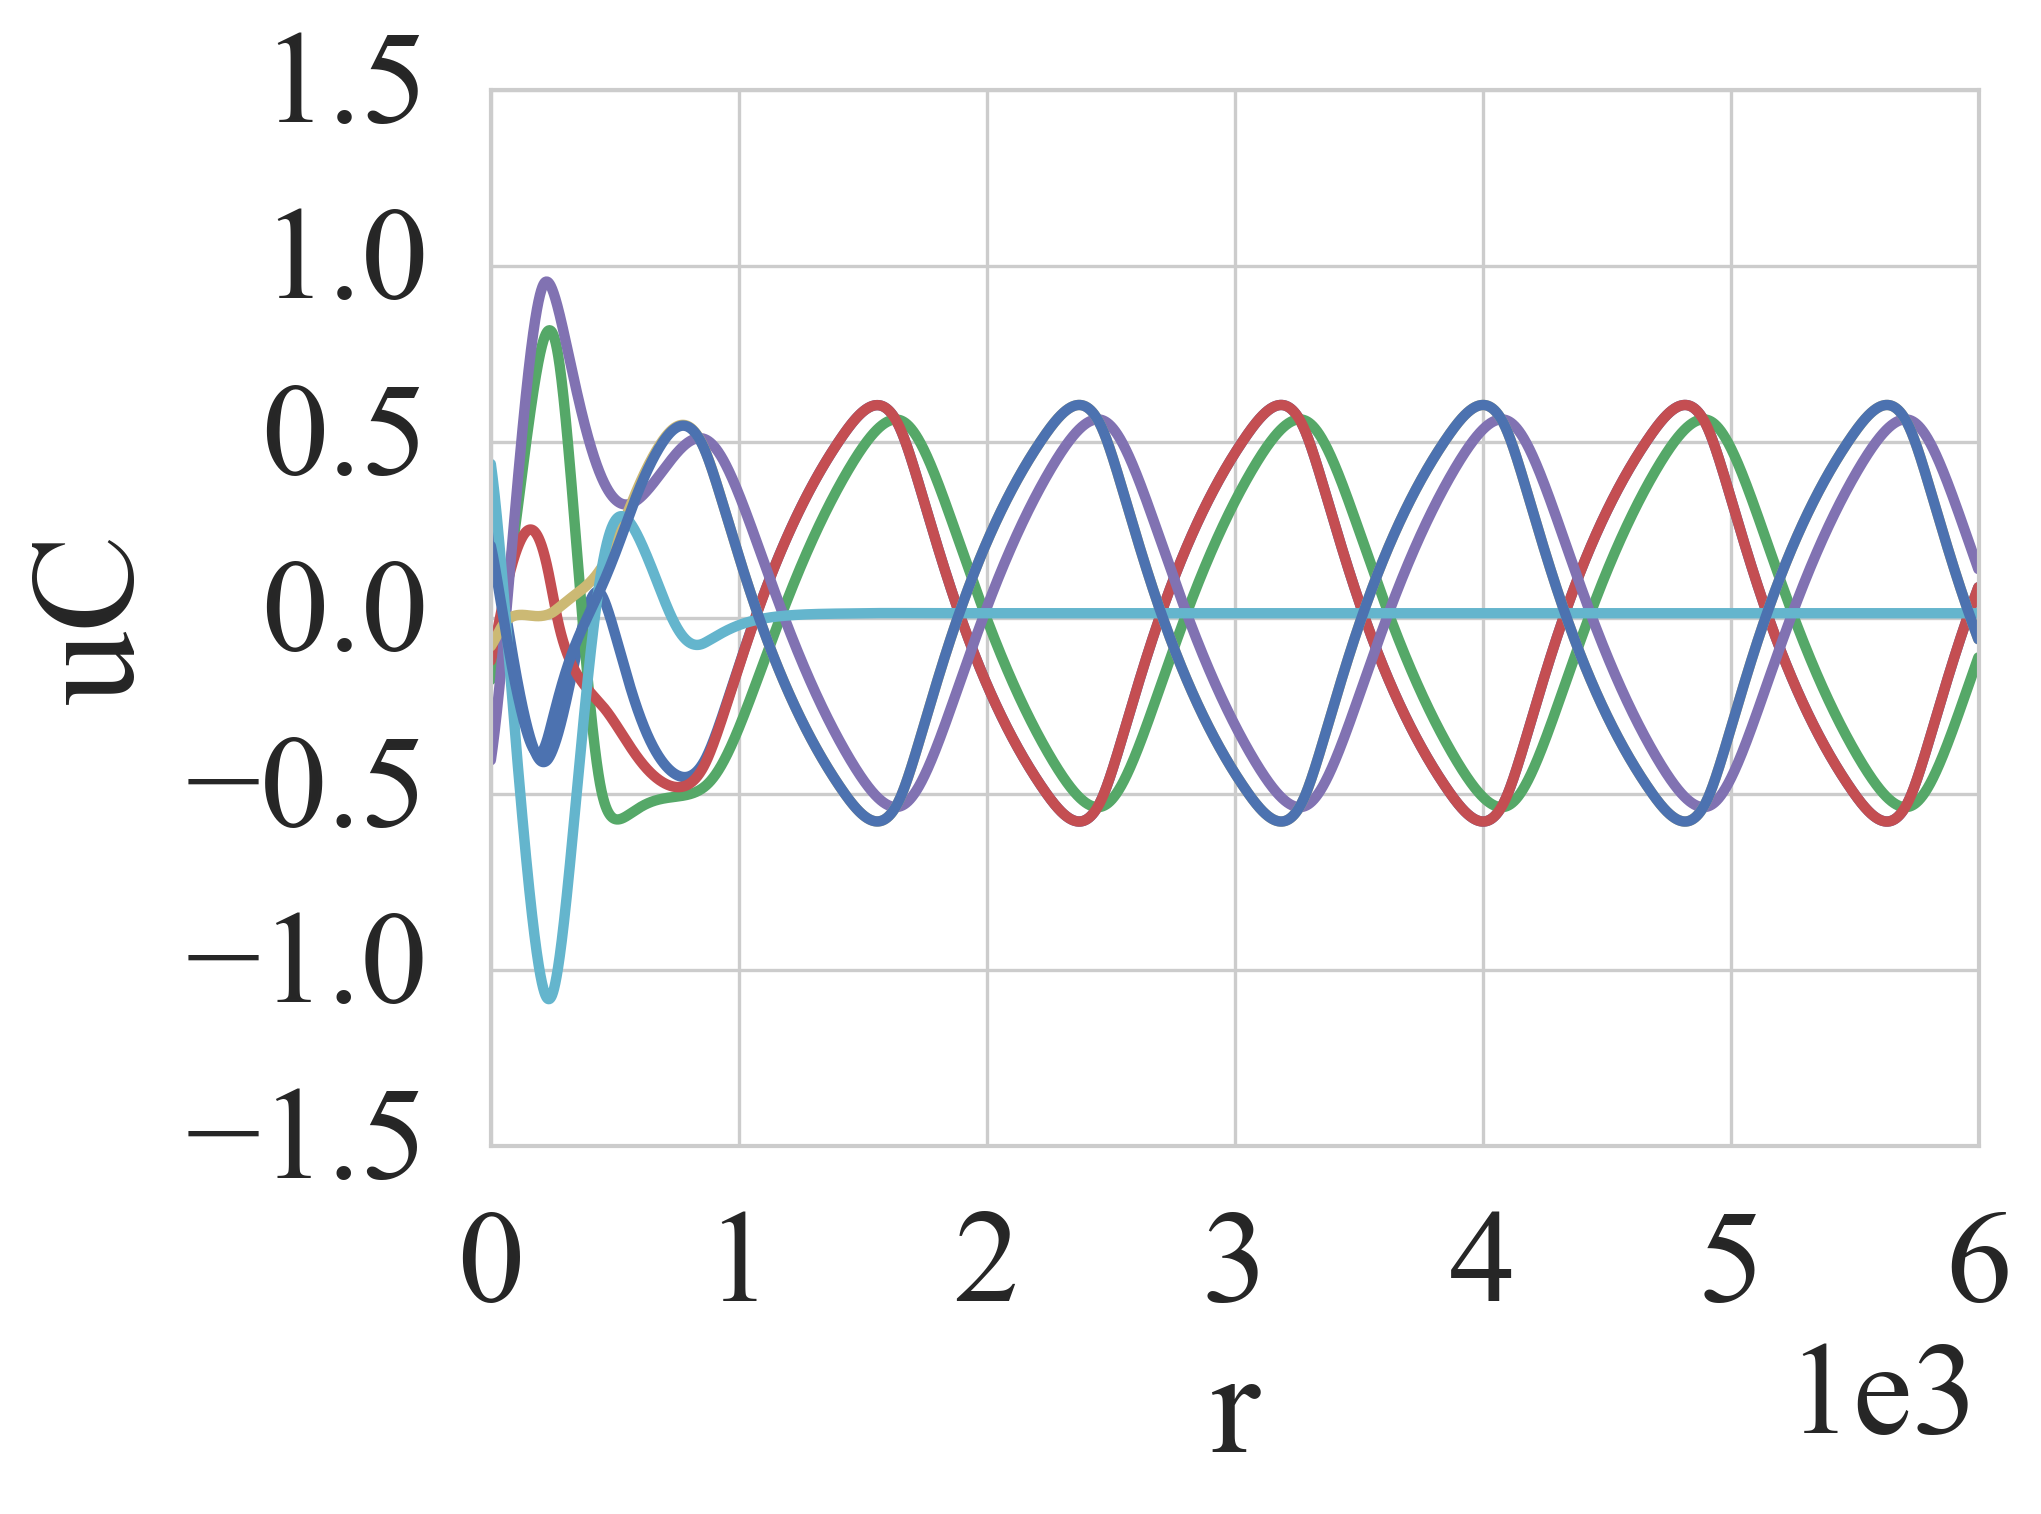
\includegraphics[width=0.4\linewidth,keepaspectratio]{./simulation/dumbbell/dumbbell_3_1_uC_asymmetric.png}\label{fig:dumbbell_uC_asymmetric}}
			
			\caption[Simulation - Dumbbell graph]{A \Pn designed to mimic aspects of the delay-coupled oscillator model of \P.}
			\label{fig:dumbbell}
		\end{figure}

		\FloatBarrier

	\subsection{Physarum Elements and Changing Topology}

		Finally, we show that the model is capable of adapting to changes in the topology of the underlying \Pn. This is not surprising given that at the heart of our model are electronic circuits. It is possible that a formal proof of this property can be obtained.

		Here we present numerical evidence based on modifying the graph presented in the previous section, see \Fref{fig:dumbbell_graph}. Needless to say, \Fref{fig:dumbbell_graph_legend} defines a color coding which serves as a legend for the plots of \Fref{fig:robustness}.

		In \Fref{fig:dumbbell_ip_changing} and \Fref{fig:ddumbbell_uC_changing} the channel edge $(5,0)$ was removed from the \Pn at point $r=4000$ and reinserted at $r=8000$. The plots illustrate how oscillations cease immediately at $r = 4000$ in favor of steady flow of opposite sign through the two cycles. The same speedy adaptation is seen in reverse when the channel edge returns at $r= 8000$.

		The procedure of changes is more complicated in  \Fref{fig:dumbbell_ip_changing_2} and \Fref{fig:dumbbell_uC_changing_2}. Here we start the simulation with the channel edge $(5,0)$ as well as one edge from the right cycle $(2,0)$ removed. As expected the plots show both the behavior of a path of length $2$ as well as constant flow in the remaining cycle. At $r = 4000$ we bring back the channel edge. At this point the \Pn consists of a $3$-cycle with a path of length $3$ attached to it. Note the complex signal shown by the circuit. The influence of the path is clearly visible, inducing oscillations in the cycle. At $r=8000$ we bring back the remaining edge and observe how the system jumps back to the expected initial behavior.


		\begin{figure}
			\centering
			
			\subfloat[][]{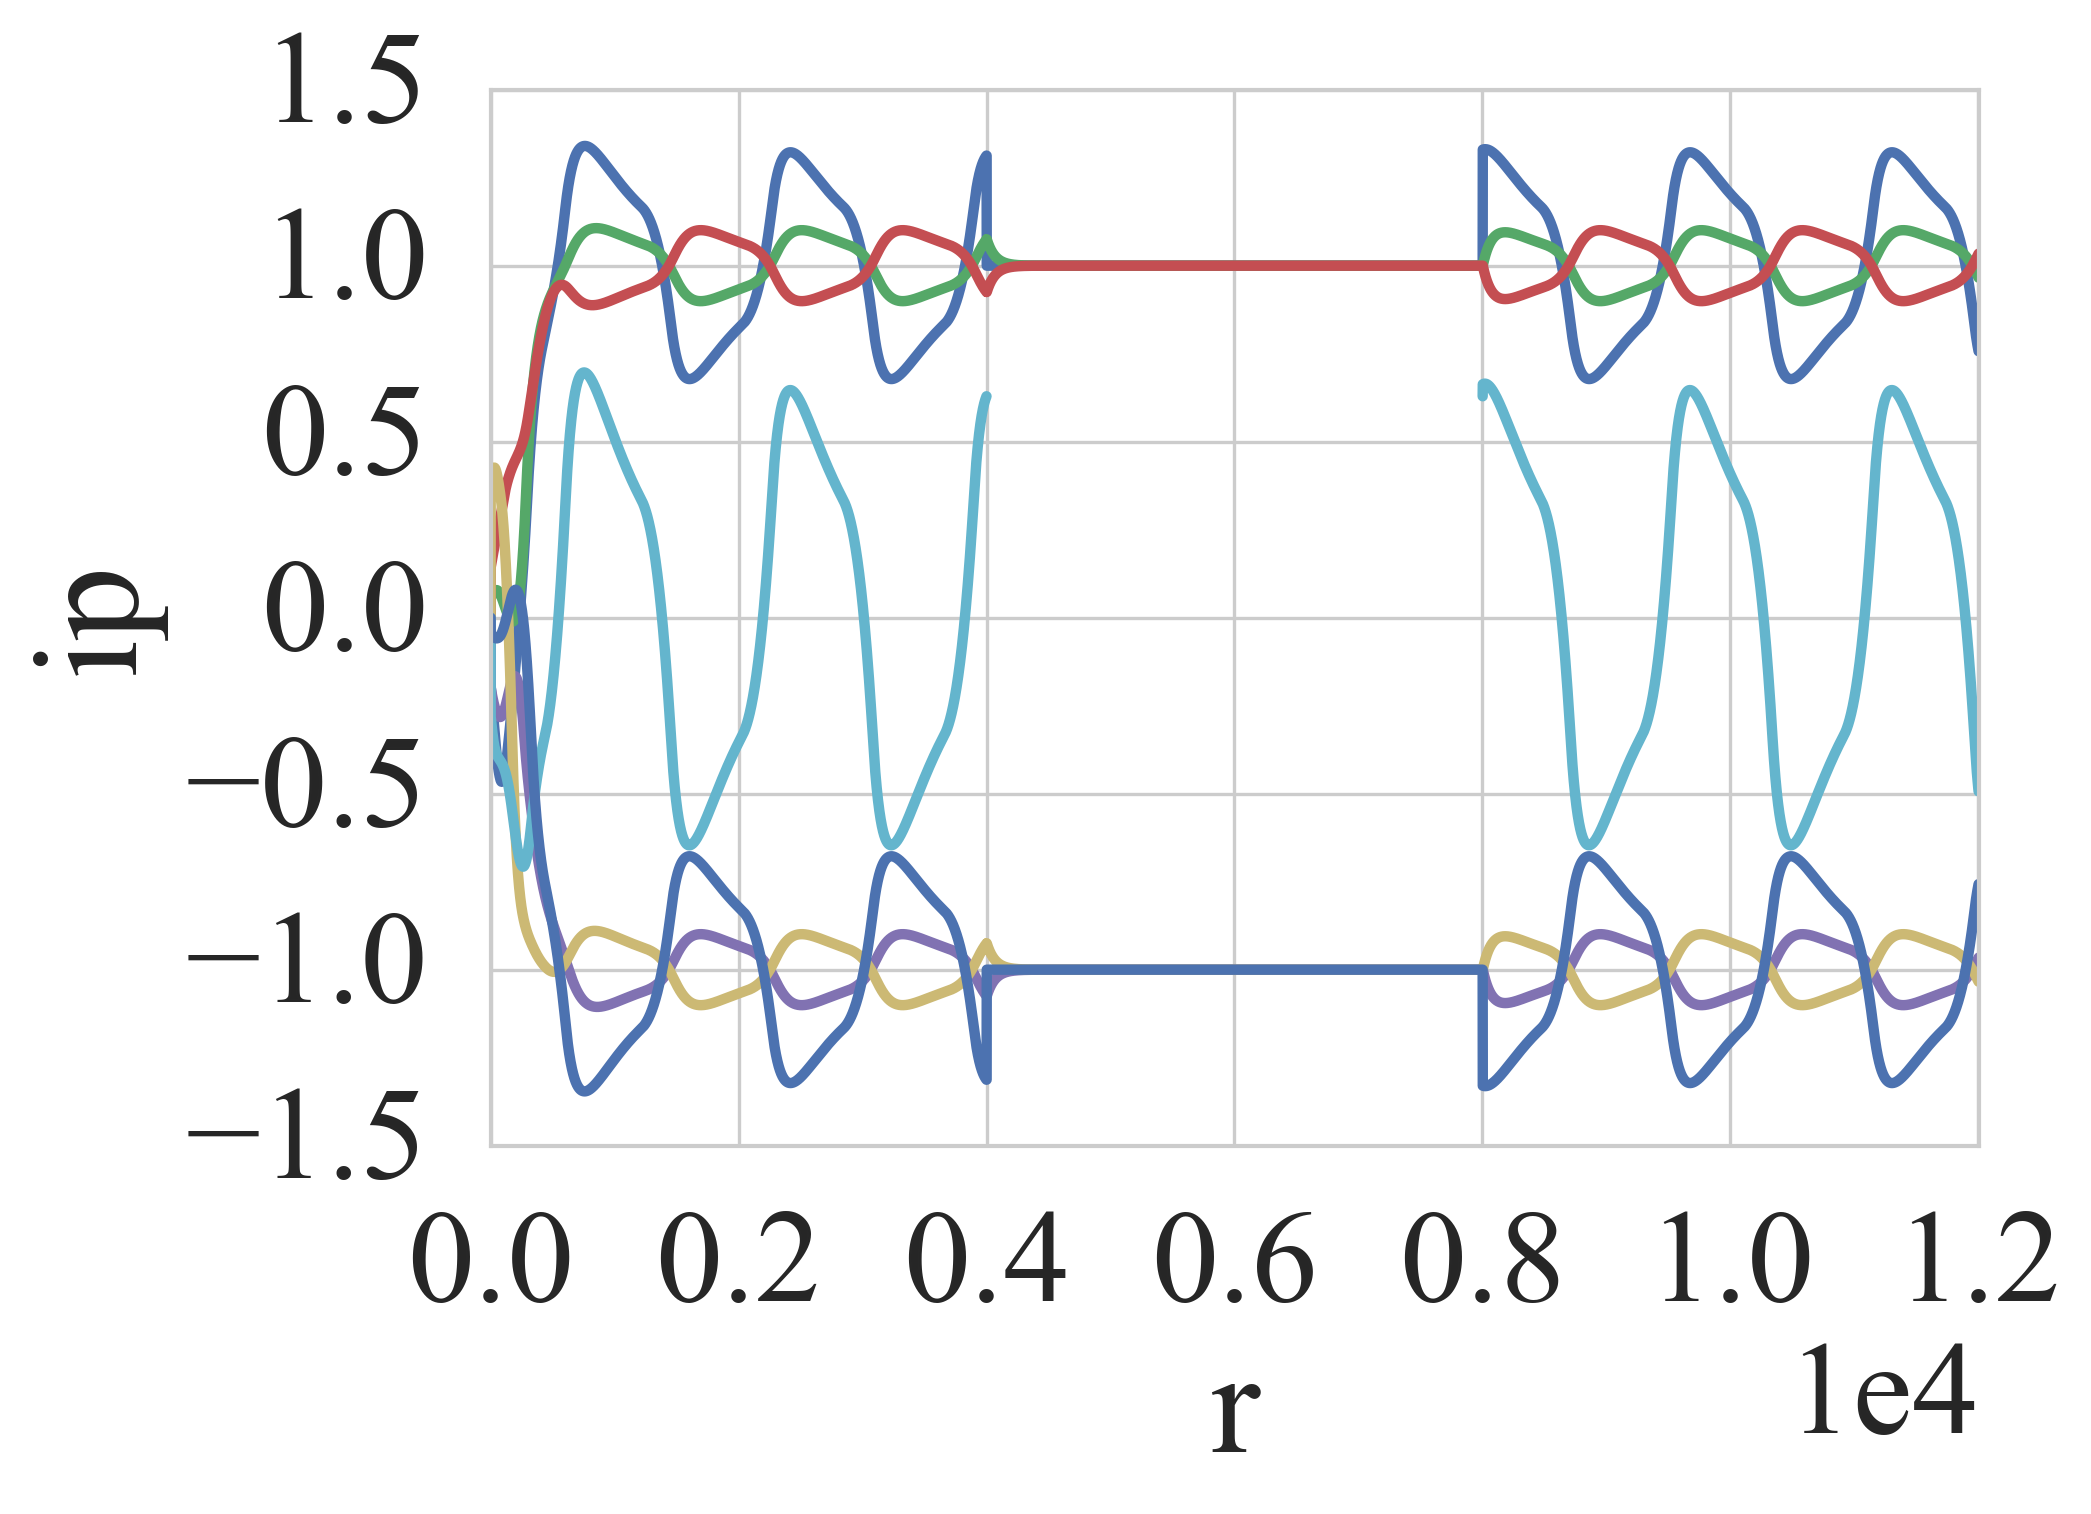
\includegraphics[width=0.4\linewidth,keepaspectratio]{./simulation/dumbbell/dumbbell_ip_changing.png}\label{fig:dumbbell_ip_changing}}\qquad
			\subfloat[][]{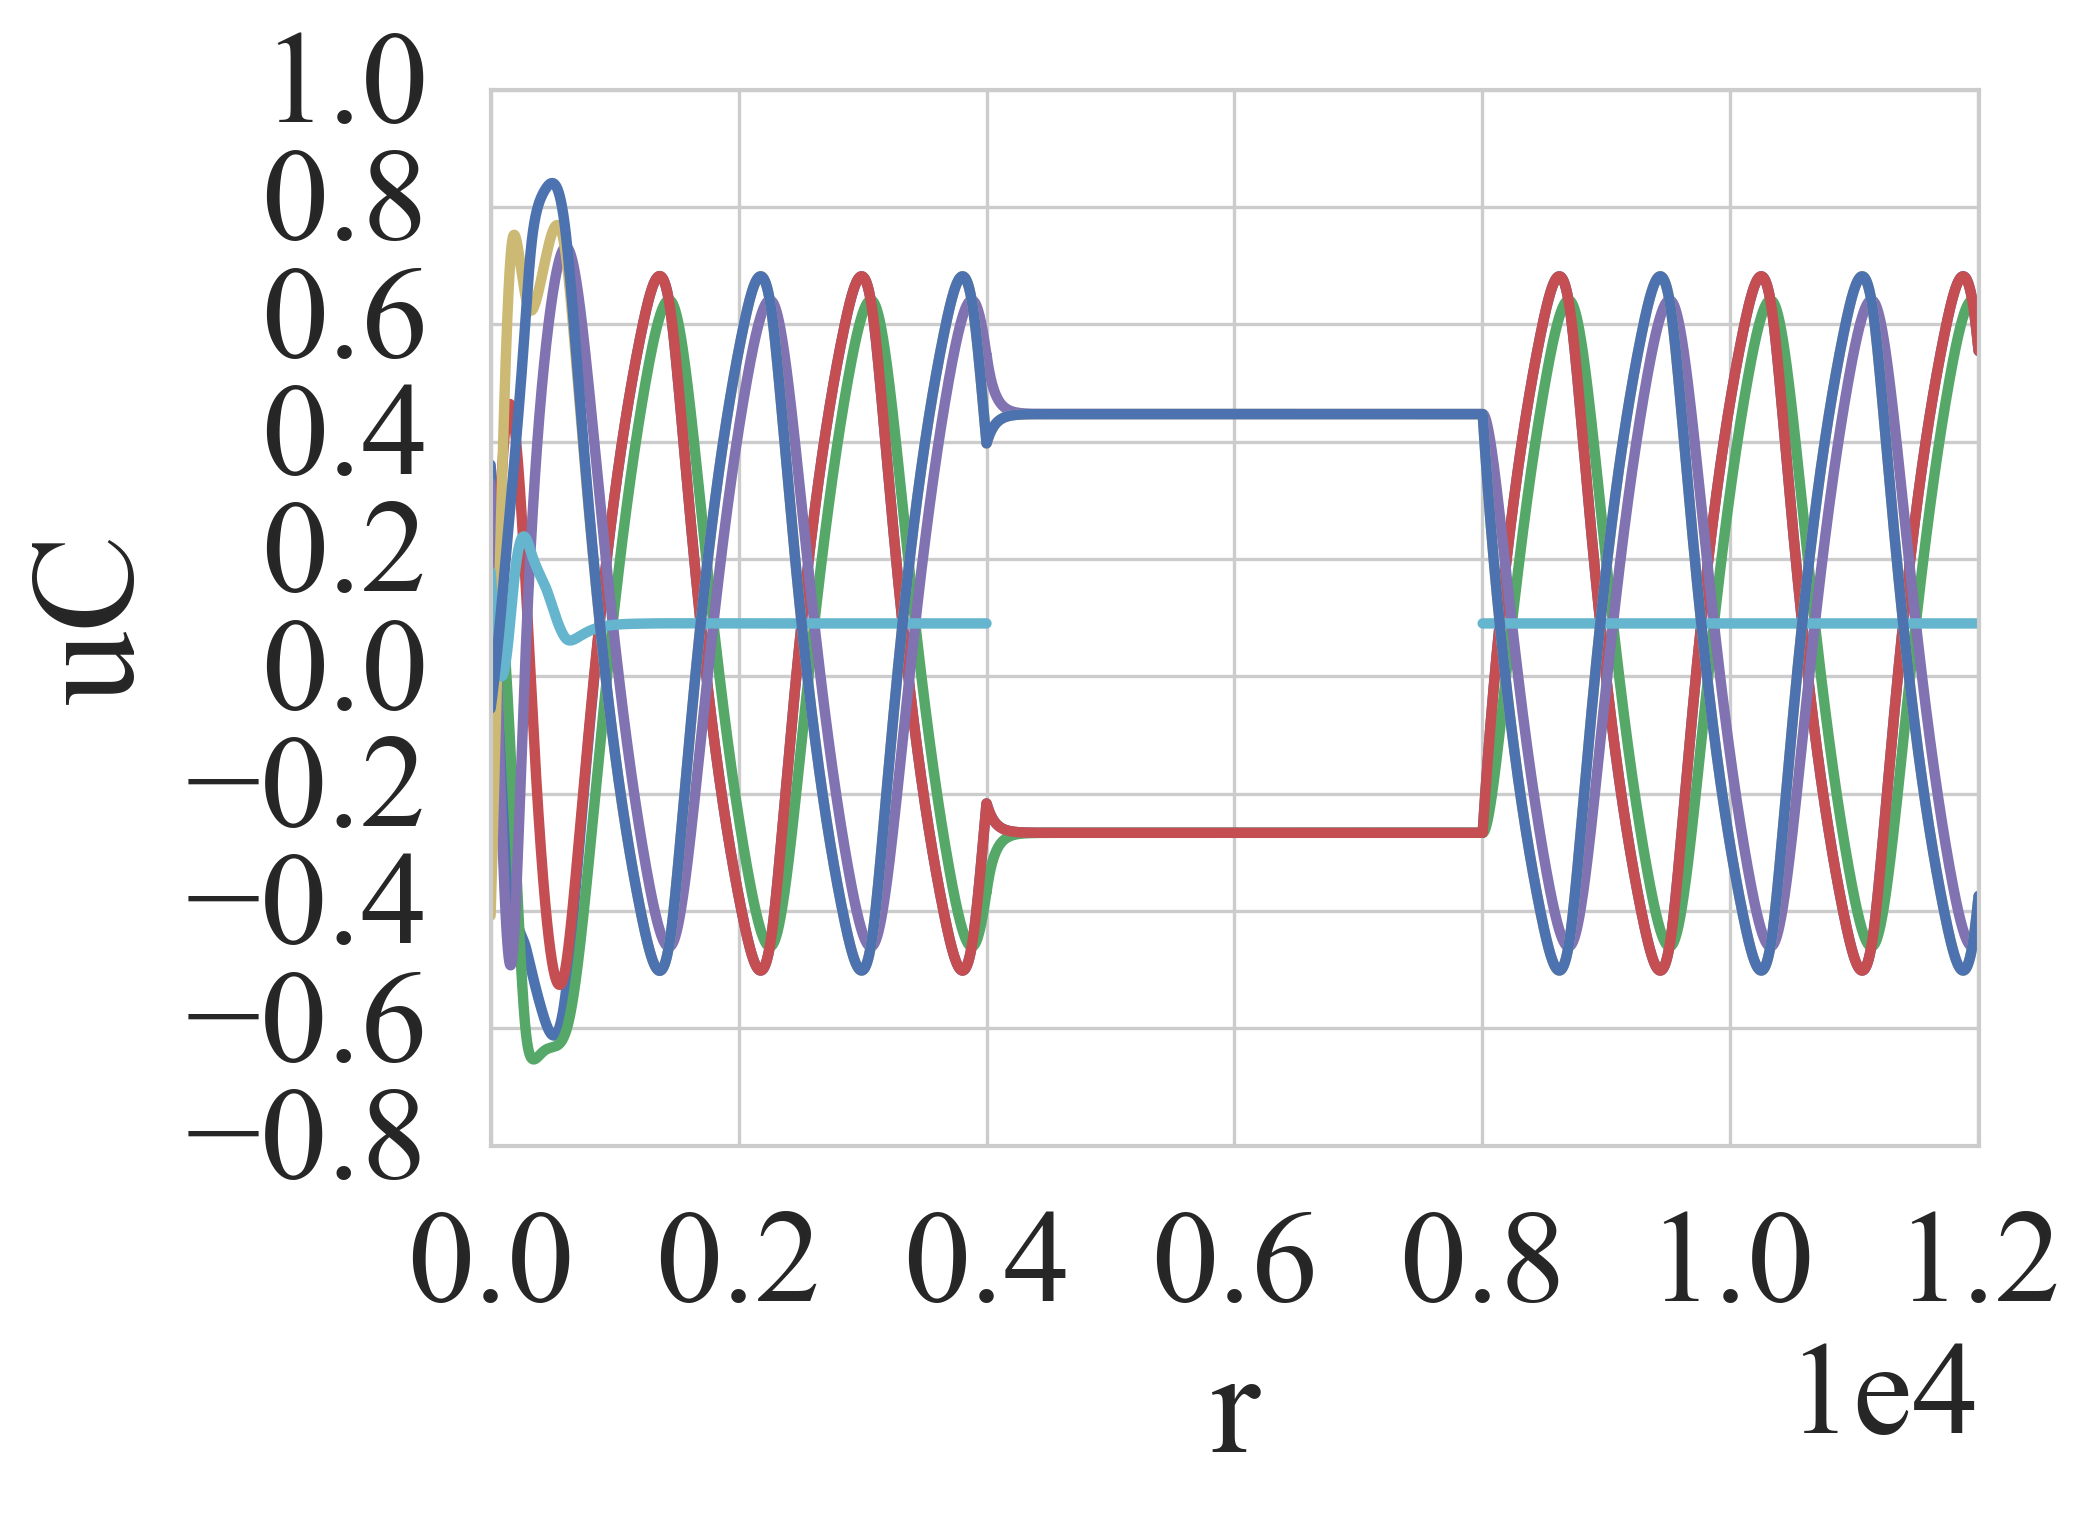
\includegraphics[width=0.4\linewidth,keepaspectratio]{./simulation/dumbbell/dumbbell_uC_changing.png}\label{fig:ddumbbell_uC_changing}}
			\newline
			\subfloat[][]{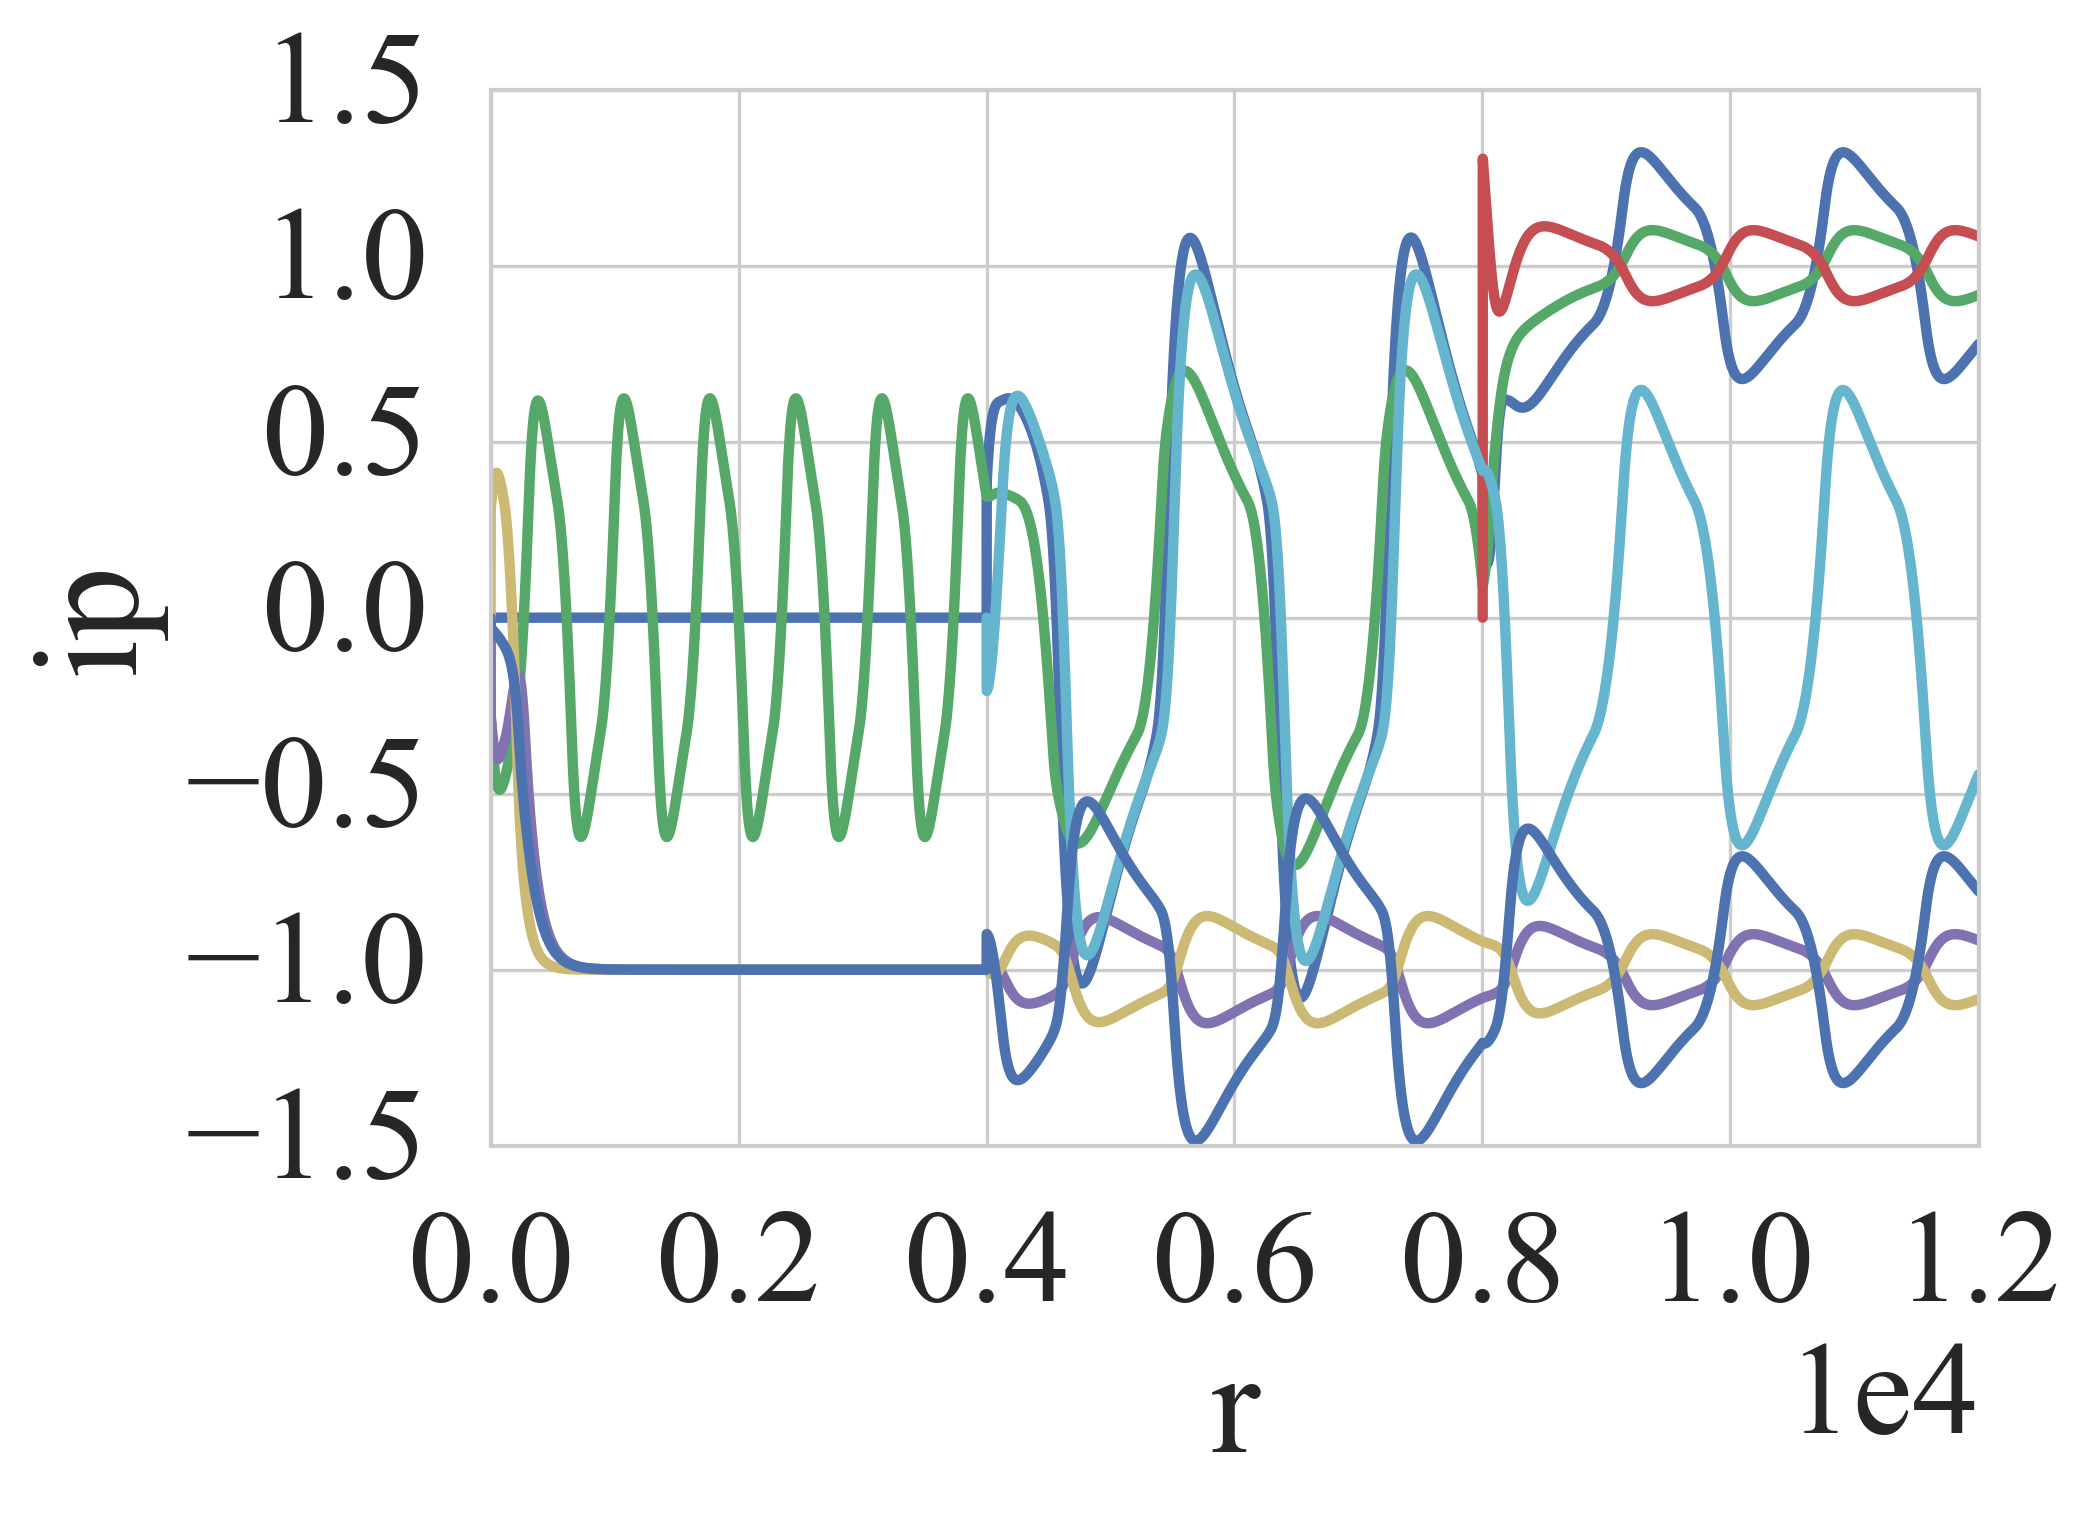
\includegraphics[width=0.4\linewidth,keepaspectratio]{./simulation/dumbbell/dumbbell_ip_changing_2.png}\label{fig:dumbbell_ip_changing_2}}\qquad
			\subfloat[][]{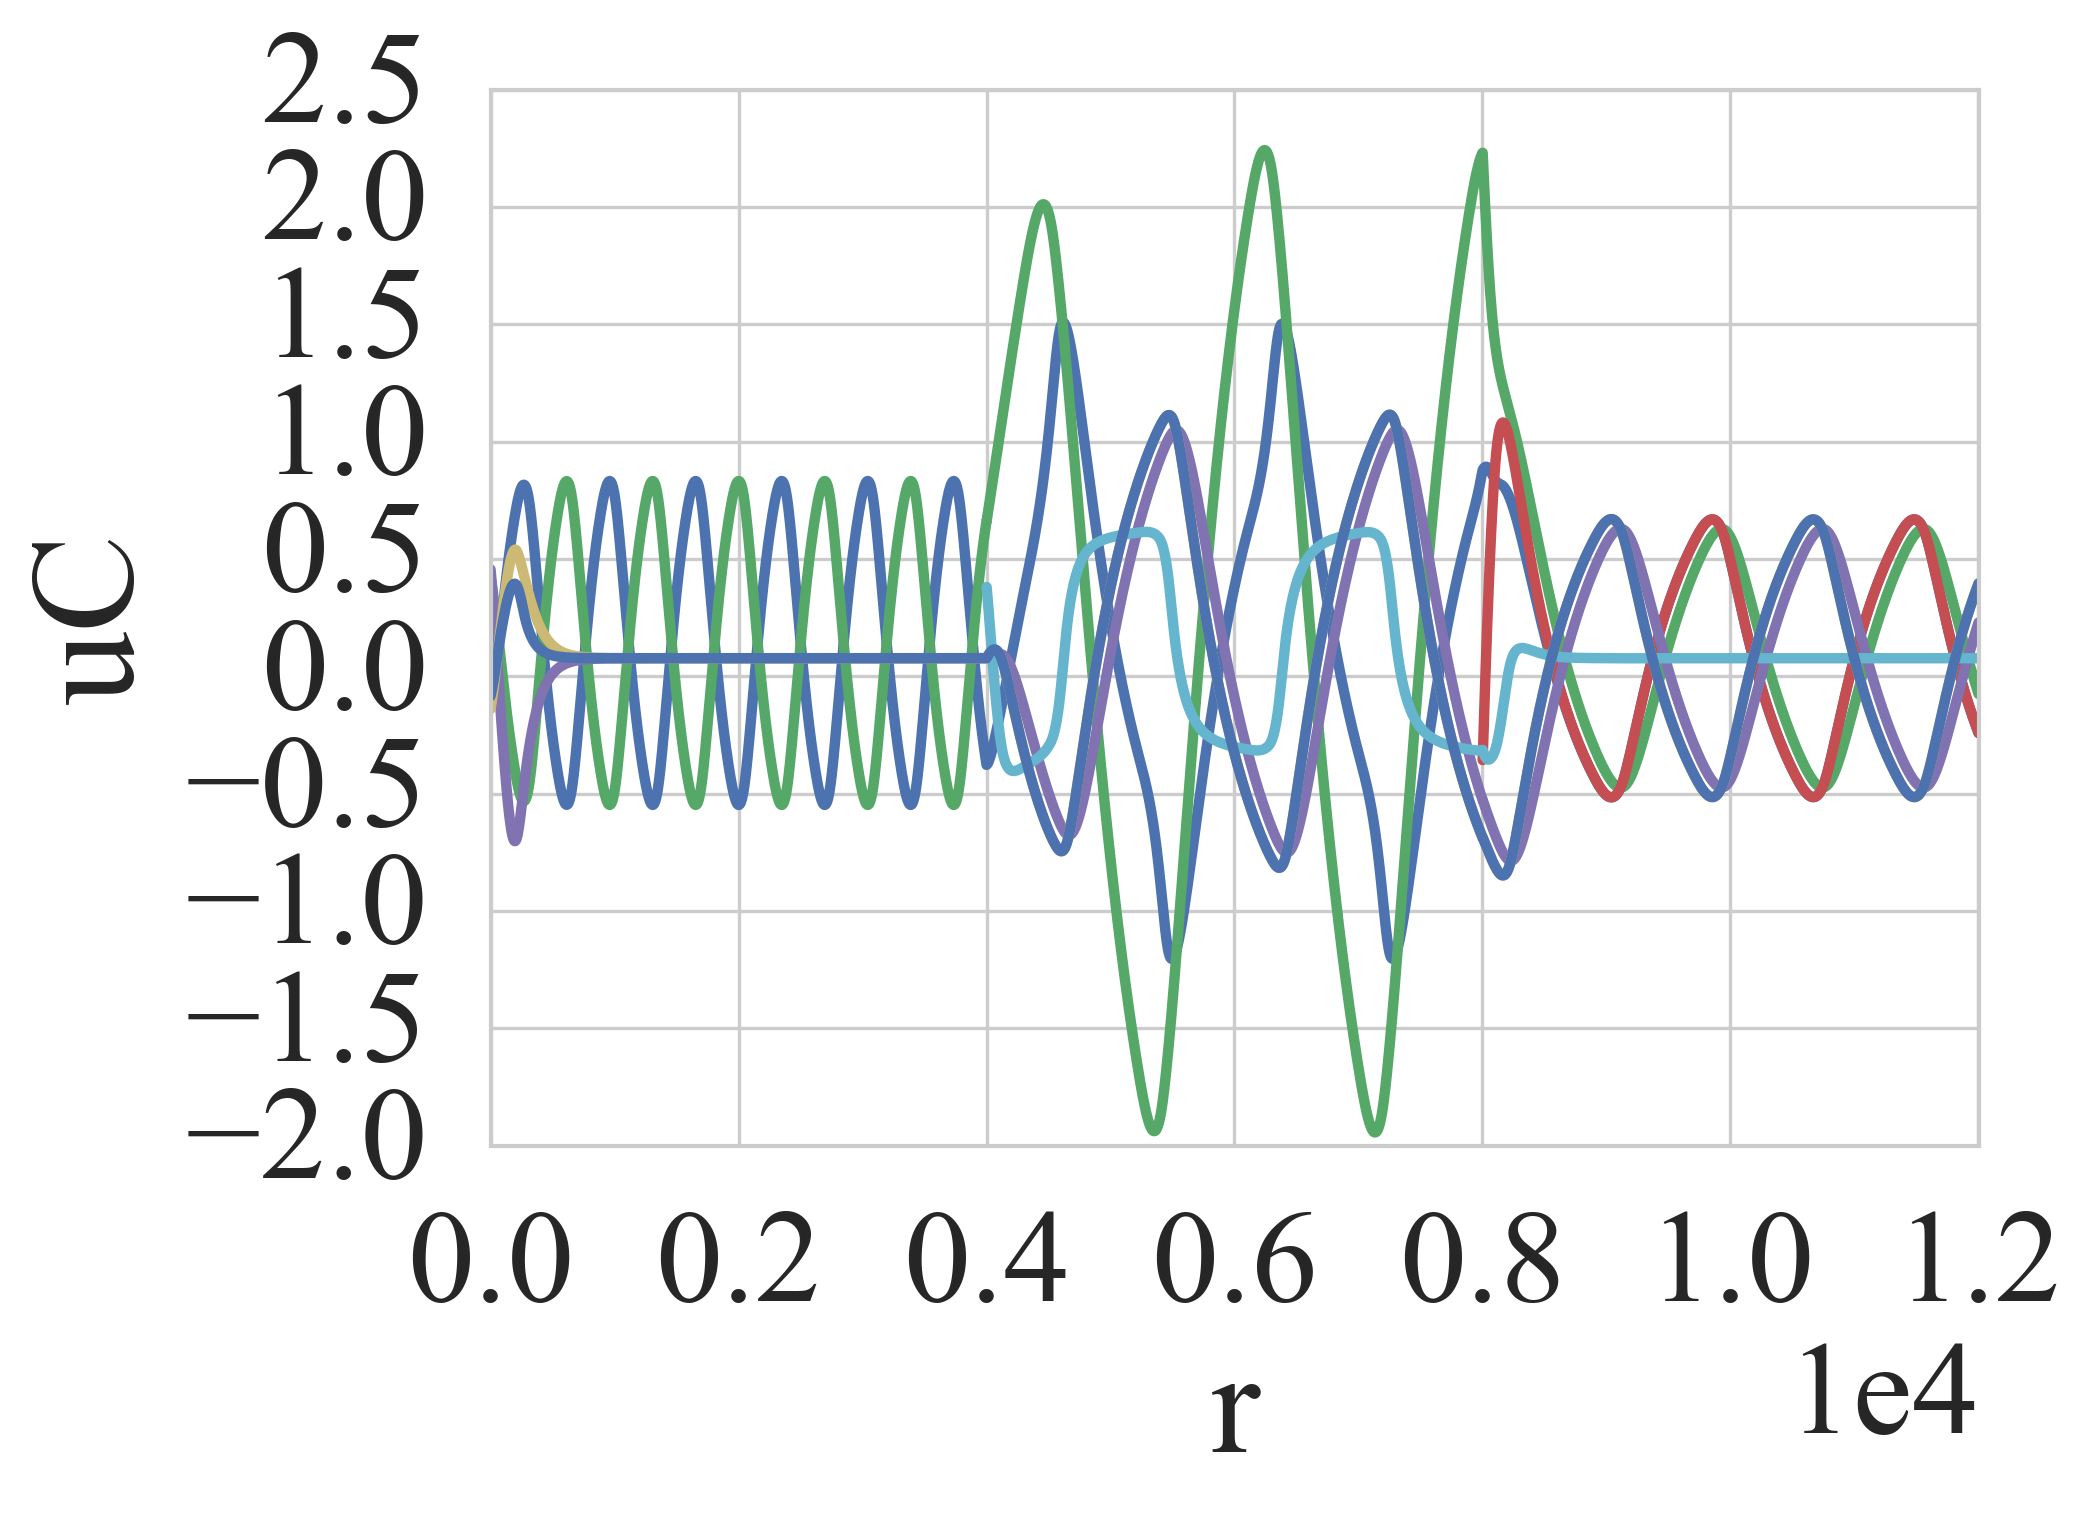
\includegraphics[width=0.4\linewidth,keepaspectratio]{./simulation/dumbbell/dumbbell_uC_changing_2.png}\label{fig:dumbbell_uC_changing_2}}
			
			\caption[Simulation - Changing topology]{\Pns changing every $4000$ rounds.}
			\label{fig:robustness}
		\end{figure}

		These preliminary examples illustrate that changes in topology are naturally accommodated by the model. A more systematic investigation is a possible task for the future. Note, that when obtaining formal robustness properties for \Pns one may start by scanning related literature for classical electronic circuits.

		\FloatBarrier